\documentclass[12pt,prb,aps]{revtex4-1}
\usepackage{amsmath}           		          	
\usepackage{graphicx,epstopdf}					
\usepackage{amssymb}
\usepackage{fullpage}
\usepackage{color}
\usepackage{esint}
\pdfoutput = 1 
\newcommand {\bxi}{\mbox{\boldmath$\xi$}}
\allowdisplaybreaks

\begin{document}
\title{Calculation of Tearing Mode Stability in an Inverse Aspect-Ratio Expanded Tokamak Plasma Equilibrium: Reference Version}
\author{Richard Fitzpatrick\,\footnote{rfitzp@utexas.edu}}
\affiliation{Institute for Fusion Studies, Department of Physics, University of Texas at Austin, Austin, TX 78712}

\begin{abstract}
The   tearing mode stability of an inverse aspect-ratio expanded tokamak plasma equilibrium of general
shape  is investigated using asymptotic matching techniques. Particular emphasis is placed on the
conservation of toroidal electromagnetic angular momentum.
% The TJ code, which is a specific implementation of theresults of the investigation, is described. 
\end{abstract}
\maketitle

\section{Introduction} 
The calculation of the tearing mode stability of a high temperature, axisymmetric,  tokamak plasma equilibrium is most efficiently formulated as  an asymptotic
matching problem.\cite{fkr} In such a problem, the  plasma is  divided into two regions. In the ``outer region'', which comprises most
of the plasma, the tearing perturbation is described by the equations of linearized, marginally-stable, ideal magnetohydrodynamics (which, in the following, are
referred to as the ``ideal-MHD'' equations). (See Sect.~\ref{mhd}.)
However, these equations become singular on so-called ``rational'' magnetic flux-surfaces at which the perturbed magnetic field resonates with the equilibrium field. In the so-called ``inner region'', which
consists of a set of narrow layers centered on the various rational surfaces, non-ideal-MHD effects such as plasma inertia, resistivity, and
viscosity become important. The growth-rate and angular rotation frequency of the reconnected magnetic flux at a given rational
surface (numbered $k$) are fixed by asymptotically matching the resistive layer
solution in the associated segment of the inner region, which is characterized by a dimensionless complex quantity ${\mit\Delta}_k$,  to the ideal-MHD solution in the outer region. In a realistic axisymmetric tokamak  plasma equilibrium, tearing
perturbations with different toroidal mode numbers are independent of one another, whereas perturbations with different poloidal
mode numbers are coupled together via toroidicity and the non-circular shaping of equilibrium magnetic flux-surfaces.\cite{con0}
Consequently, for a tearing perturbation with a given toroidal mode number, 
 the ${\mit\Delta}_k$ values associated with  the various rational surfaces in the plasma are interrelated via a matrix equation.\cite{cht} [See Eq.~(\ref{e317u}).]

In general, the  determination of the elements of the matrix equation that links the various ${\mit\Delta}_k$ values from the ideal-MHD equations 
in the outer region is an exceptionally challenging computational task.\cite{connor,nish,gal,pletz,pletz1,
tokuda,brennan,ham,ham1,ham2,am1,am2,am3,aglas,aglas1,aglas2}
One way of greatly reducing the complexity of this task is to employ an inverse aspect-ratio expanded plasma equilibrium.\cite{greene,gim} In such an equilibrium,
the metric elements of the flux-coordinate system can be expressed analytically in terms of a relatively small number of  flux-surface functions,
which represents a major simplification.\cite{con0} Another significant advantage of an inverse aspect-ratio expanded equilibrium is that the magnetic perturbation in the plasma can be efficiently 
matched to an exterior vacuum solution  that is expressed as an expansion in toroidal functions.\cite{am1} The alternative approach of using a Green's
function solution in the vacuum region is much more computationally intensive.\cite{chance,xu}  

 The inverse aspect-ratio expansion approach to determining tearing mode stability in tokamak plasmas 
was first presented in Ref.~\onlinecite{connor} in a calculation that  features triplets of  poloidal harmonics coupled via toroidicity. 
The
inverse aspect-ratio expansion approach was extended in Ref.~\onlinecite{am1} in a calculation that features septuplets of poloidal harmonics coupled via toroidicity, flux-surface elongation, and
flux-surface triangularity. In this paper, we  generalize the inverse aspect-ratio expansion  approach to allow for an {\em arbitrary}\/ number of poloidal harmonics coupled
by flux-surfaces of {\em general}\/ shape. Furthermore, unlike Refs.~\onlinecite{connor} and \onlinecite{am1}, we do not assume that the plasma
equilibrium 
is up-down-symmetric. 

This paper is organized as follows. In Sect.~\ref{geq}, we examine a general tokamak plasma equilibrium. In Sect.~\ref{opde}, we
derive the so-called ``outer-region  partial differential equations (p.d.e.s)", which are a set of two coupled second-order p.d.e.s that control   the ideal-MHD solution in the outer region. In
Sect.~\ref{sode}, we derive the so-called ``outer region ordinary differential equations  (o.d.e.s)'', which are a large set of coupled first-order 
o.d.e.s that control the ideal-MHD solution in the outer region. We also demonstrate that these o.d.e.s conserve toroidal electromagnetic
angular momentum. In Sect.~\ref{snus}, we discuss the general behavior of the outer-region o.d.e.s in the vicinity of a rational surface. 
In Sect.~\ref{vacxx}, we obtain the general boundary condition satisfied by the outer-region o.d.e.s at the plasma/vacuum interface, on the assumption that
the region surrounding the plasma does not contain any non-axisymmetric currents. We also demonstrate that these boundary conditions conserve
toroidal electromagnetic angular momentum. In Sect.~\ref{large}, we introduce the aspect-ratio expanded tokamak equilibrium, and determine the
specific forms of the outer-region o.d.e.s. In Sect.~\ref{etm}, we calculate the matrix equation that constitutes the tearing mode dispersion relation, and
demonstrate that this equation must be Hermitian in order to conserve toroidal electromagnetic angular momentum. In Sect.~\ref{rmp}, 
we discuss how the tearing mode dispersion relation is modified by non-axisymmetric currents flowing in
 resonant magnetic perturbation (RMP) coils external to the plasma. We also derive expressions for the toroidal electromagnetic
torques exerted at the various rational surfaces in the plasma by the RMP coils.
% In Sect.~\ref{tj}, we discuss the
%TJ code, which is a specific implementation of the theory presented in Sects.~\ref{geq}--\ref{rmp}. Finally, the paper is summarized in Sect.~\ref{sum}.

\section{General Plasma Equilibrium}\label{geq}
\subsection{Normalization}\label{coords}
All lengths in this paper are normalized to  the major radius of the plasma magnetic axis, $R_0$. All magnetic field-strengths
are normalized to the  toroidal field-strength at the magnetic axis, $B_0$. All currents are normalized to $B_0\,R_0/\mu_0$. All current densities are normalized to $B_0/(\mu_0\,R_0)$.  All plasma pressures are normalized to $B_0^{\,2}/\mu_0$.
All toroidal electromagnetic torques are normalized to $B_0^{\,2}\,R_0^{\,3}/\mu_0$. 

\subsection{Axisymmetric Tokamak Plasma Equilibrium}\label{s3}
Let $R$, $\phi$, $Z$ be right-handed cylindrical coordinates whose Jacobian 
is
\begin{equation}
(\nabla R\times \nabla\phi\cdot\nabla Z)^{-1} = R.
\end{equation}
Note that $|\nabla\phi|=1/R$. 

Let $r$, $\theta$, $\phi$ be right-handed flux-coordinates whose
Jacobian is\,\cite{connor,bussac}
\begin{equation}\label{jac}
{\cal J}(r,\theta)\equiv (\nabla r\times \nabla\theta\cdot\nabla\phi)^{-1} \equiv R\left(\frac{\partial R}{\partial\theta}\,\frac{\partial Z}{\partial r} -\frac{\partial R}{\partial r}\,\frac{\partial Z}{\partial \theta}\right)= r\,R^{\,2}.
\end{equation}
Note that $r=r(R,Z)$ and $\theta=\theta(R,Z)$. 
The magnetic axis corresponds to $r=0$. The inboard mid-plane corresponds to $\theta=0$. 

Consider an axisymmetric tokamak equilibrium\,\cite{gs1} whose magnetic field takes the form\,\cite{connor,am1}
\begin{equation}
{\bf B}(r,\theta) = f(r)\,\nabla\phi\times \nabla r + g(r)\,\nabla\phi = f\,\nabla(\phi-q\,\theta)\times \nabla r,
\end{equation}
where
\begin{equation}\label{q}
q(r) = \frac{r\,g}{f}
\end{equation}
is the safety-factor (i.e., the inverse of the rotational transform). Note that ${\bf B}\cdot\nabla r=0$, which implies that $r$ is a magnetic flux-surface label.
We require $g=1$ on the magnetic axis in order to ensure that the normalized toroidal magnetic field-strength at the  axis is unity.  

It is easily demonstrated that
\begin{align}
B^{\,r}&={\bf B}\cdot\nabla r= 0,\label{bup1}\\[0.5ex]
B^{\,\theta} &={\bf B}\cdot\nabla \theta= \frac{f}{r\,R^{\,2}},\label{bup2}\\[0.5ex]
B^{\,\phi} &={\bf B}\cdot\nabla \phi= \frac{g}{R^{\,2}},\label{bup3}\\[0.5ex]
B_r &={\cal J}\,\nabla\theta\times\nabla\phi\cdot{\bf B}= -r\,f\,\nabla r\cdot\nabla\theta,\label{bdown1}\\[0.5ex]
B_\theta &={\cal J}\,\nabla\phi\times\nabla r\cdot{\bf B}= r\,f\,|\nabla r|^2,\\[0.5ex]
B_\phi &={\cal J}\,\nabla r\times\nabla \theta \cdot{\bf B}= g,\label{bdown3}
\end{align}
where use has been made of the results and notation of Sect.~\ref{s2}. 

The Maxwell equation (neglecting the displacement current, because tearing modes are comparatively low-frequency phenomena)
${\bf J}= \nabla\times{\bf B}$
yields
\begin{align}
{\cal J}\,J^{\,r} &= \frac{\partial B_\phi}{\partial \theta} =0,\label{jup1}\\[0.5ex]
{\cal J}\,J^{\,\theta} &= -\frac{\partial B_\phi}{\partial r} = - g',\label{jup2}\\[0.5ex]
{\cal J}\,J^{\,\phi}&= \frac{\partial B_\theta}{\partial r} -\frac{\partial B_r}{\partial\theta}=\frac{\partial}{\partial r}\!\left(r\,f\,|\nabla r|^2\right)+ \frac{\partial}{\partial\theta}\!\left(r\,f\,\nabla r\cdot\nabla\theta\right),\label{jup3}
\end{align}
where ${\bf J}$ is the equilibrium current density, $'\equiv d/dr$, and use has been made of  Eqs.~(\ref{bdown1})--(\ref{bdown3}) and (\ref{curl1})--(\ref{curl3}).

Equilibrium force balance requires that
\begin{equation}\label{e15c}
 \nabla P={\bf J}\times {\bf B},
\end{equation}
where $P(r)$ is the equilibrium scalar plasma pressure. Here, for the sake of simplicity, we have neglected the small centrifugal modifications to force balance due to subsonic plasma
rotation.\cite{flow,flow1}
It follows that 
\begin{align}\label{eg1}
P'&= {\cal J}(J^{\,\theta}\,B^{\,\phi}-J^{\,\phi}\,B^{\,\theta})= -g'\,\frac{g}{R^{\,2}} - \frac{f}{r\,R^{\,2}}\left[\frac{\partial}{\partial r}\!\left(r\,f\,|\nabla r|^2\right)+ \frac{\partial}{\partial\theta}\!\left(r\,f\,\nabla r\cdot\nabla\theta\right)\right],
\end{align}
where use has been made of Eqs.~(\ref{bup1})--(\ref{bup3}),  (\ref{jup1})--(\ref{jup3}), and (\ref{crossdown1})--(\ref{crossdown3}). The
other two components of Eq.~(\ref{e15c}) are identically zero. 

Equation~(\ref{eg1}) yields the {\em Grad-Shafranov equation},\cite{gs1}
\begin{equation}\label{gs}
\frac{f}{r}\,\frac{\partial}{\partial r}\!\left(r\,f\,|\nabla r|^2\right) +\frac{f}{r}\,\frac{\partial}{\partial\theta}\!\left(r\,f\,\nabla r\cdot\nabla\theta\right)+g\,g' + R^{\,2}\,P'=0.
\end{equation}
It follows from Eqs.~(\ref{q}), (\ref{jup3}), and (\ref{gs}) that
\begin{equation}\label{jup3a}
{\cal J}\,J^{\,\phi} = -q\,g' - \frac{r\,R^{\,2}\,P'}{f}.
\end{equation}
It is clear from Eqs.~(\ref{jup2}) and (\ref{jup3a}) that $g'=P'=0$ in the  current-free ``vacuum'' region surrounding the plasma.
We shall also assume that $g'=P'=0$ at the plasma/vacuum interface, so as to ensure that the equilibrium plasma
current density is zero at the interface. 

\section{Derivation of Outer-Region P.D.E.s}\label{opde}
\subsection{Introduction}
The outer-region p.d.e.s  were first presented in Ref.~\onlinecite{connor} without an explicit
derivation. However, the derivation is sufficiently non-obvious that it is worth outlining in this section. 

\subsection{Governing Equations}\label{mhd}
In the outer region, the perturbed plasma equilibrium satisfies the  ideal-MHD equations\,\cite{connor,am1,am3,gs1}
\begin{align}
{\bf b} &= \nabla\times (\bxi\times {\bf B}),\label{e21}\\[0.5ex]
\nabla p &={\bf j}\times {\bf B}  +{\bf J}\times {\bf b},\label{e22}\\[0.5ex]
{\bf j} &= \nabla\times {\bf b},\label{e23}\\[0.5ex]
p&= -\bxi\cdot\nabla P,\label{e24}
\end{align}
where $\bxi(r,\theta,\phi)$ is the plasma displacement, ${\bf b}(r,\theta,\phi)$ the perturbed magnetic field,
${\bf j}(r,\theta,\phi)$ the perturbed current density, and $p(r,\theta,\phi)$ the perturbed scalar pressure. 
Let us assume that all perturbed quantities vary with the toroidal angle, $\phi$, as $\exp(-{\rm i}\,n\,\phi)$, where the real positive integer $n$ is the
toroidal mode number of the tearing mode. For example, $p(r,\theta,\phi) = p(r,\theta)\,\exp(-{\rm i}\,n\,\phi)$. 

\subsection{Radial Plasma Displacement}
Equations~(\ref{crossdown2}) and (\ref{crossdown3}) yield
\begin{align}
(\bxi\times {\bf B})_\theta&= {\cal J}\,(\xi^{\,\phi}\,B^{\,r} - \xi^{\,r}\,B^{\,\phi}) = -{\cal J}\,B^{\,\phi}\,\xi^{\,r},\\[0.5ex]
(\bxi\times {\bf B})_\phi &= {\cal J}\,(\xi^{\,r}\,B^{\,\theta} - \xi^{\,\theta}\,B^{\,r})= {\cal J}\,B^{\,\theta}\,\xi^{\,r},
\end{align}
where use has been made of  the fact that $B^{\,r}=J^{\,r}=0$. [See Eqs.~(\ref{bup1}) and (\ref{jup1}).]
Combining the previous two equations with  Eqs.~(\ref{e21}) and (\ref{curl1}), we obtain
\begin{align}
{\cal J}\,b^{\,r} &= \frac{\partial}{\partial\theta}\left({\cal J}\,B^{\,\theta}\,\xi^{\,r}\right)-{\rm i}\,n\,{\cal J}\,B^{\,\phi}\,\xi^{\,r}.
\end{align}
Thus, Eqs.~(\ref{jac}), (\ref{q}), (\ref{bup2}), and (\ref{bup3}) give
\begin{align}\label{e41}
r\,R^{\,2}\,b^{\,r}& = \left(\frac{\partial}{\partial\theta}-{\rm i}\,n\,q\right)y,
\end{align}
where 
\begin{align}\label{e42}
y(r,\theta) &=f\,\xi^{\,r}.
\end{align}

\subsection{Perturbed Force Balance}
According to Eq.~(\ref{e24}), 
\begin{equation}
p =-P'\,\nabla r\cdot\bxi=- P'\,\xi^{\,r}.
\end{equation}
So, the perturbed force balance equation, (\ref{e22}), yields
\begin{align}
-\frac{\partial\, (P'\,\xi^{\,r})}{\partial r} &= ({\bf j}\times {\bf B})_r+({\bf J}\times {\bf b})_r,\\[0.5ex]
-\frac{\partial\,(P'\,\xi^{\,r})}{\partial \theta}&= ({\bf j}\times {\bf B})_\theta+({\bf J}\times {\bf b})_\theta,\\[0.5ex]
{\rm i}\,n\,P'\,\xi^{\,r} &= ({\bf j}\times {\bf B})_\phi+({\bf J}\times {\bf b})_\phi,
\end{align}
giving
\begin{align}
-\frac{\partial\, (P'\,\xi^{\,r})}{\partial r} &=r\,R^{\,2}\,(j^{\,\theta}\,B^{\,\phi}-j^{\,\phi}\,B^{\,\theta}) + r\,R^{\,2}\,(J^{\,\theta}\,b^{\,\phi}-J^{\,\phi}\,b^{\,\theta}),\\[0.5ex]
-\frac{\partial\,(P'\,\xi^{\,r})}{\partial \theta}&=r\,R^{\,2}\,(j^{\,\phi}\,B^{\,r}-j^{\,r}\,B^{\,\phi}) + r\,R^{\,2}\,(J^{\,\phi}\,b^{\,r}-J^{\,r}\,b^{\,\phi}),\\[0.5ex]
{\rm i}\,n\,P'\,\xi^{\,r} &=r\,R^{\,2}\,(j^{\,r}\,B^{\,\theta}-j^{\,\theta}\,B^{\,r}) + r\,R^{\,2}\,(J^{\,r}\,b^{\,\theta}-J^{\,\theta}\,b^{\,r}),
\end{align}
where use has been made of Eqs.~(\ref{jac}) and (\ref{crossdown1})--(\ref{crossdown3}). 
Thus, according to Eqs.~(\ref{bup1})--(\ref{bup3}), (\ref{jup1}), (\ref{jup2}), and (\ref{jup3a}), 
\begin{align}
-\frac{\partial\, (P'\,\xi^{\,r})}{\partial r} &= f\,(q\,j^{\,\theta} -j^{\,\phi}) - g'\,b^{\,\phi} + \left(q\,g'+\frac{r\,R^{\,2}\,P'}{f}\right)b^{\,\theta},\label{e51}\\[0.5ex]
-\frac{\partial\,(P'\,\xi^{\,r})}{\partial \theta}&=-r\,g\,j^{\,r} - \left(q\,g'+\frac{r\,R^{\,2}\,P'}{f}\right)b^{\,r},\label{e44}\\[0.5ex]
{\rm i}\,n\,P'\,\xi^{\,r} &= f\,j^{\,r}+g'\,b^{\,r}.\label{e53}
\end{align}
It follows from Eqs.~(\ref{e42}), (\ref{e41}), and (\ref{e53}) that 
\begin{equation}\label{e54}
r\,j^{\,r} = {\rm i}\,n\,\alpha_p\,y - \frac{\alpha_g}{R^{\,2}}\left(\frac{\partial}{\partial\theta}-{\rm i}\,n\,q\right)y,
\end{equation}
where
\begin{align}
\alpha_p(r) &= \frac{r\,P'}{f^2},\label{ap}\\[0.5ex]
\alpha_g (r)&= \frac{g'}{f}.\label{ag}
\end{align}
Note that Eq.~(\ref{e44}) is trivially satisfied. Hence, of the three components of the perturbed force balance equation, only Eq.~(\ref{e51}) remains to be solved. 

\subsection{Perturbed Plasma Current Density}
Equation~(\ref{e23}) yields 
\begin{align}
r\,R^{\,2}\,j^{\,r} &= \frac{\partial b_\phi}{\partial\theta}+{\rm i}\,n\,b_\theta,\label{e57}\\[0.5ex]
r\,R^{\,2}\,j^{\,\theta} &=-{\rm i}\,n\,b_r -\frac{\partial b_\phi}{\partial r},\label{e58}\\[0.5ex]
r\,R^{\,2}\,j^{\,\phi}&= \frac{\partial b_\theta}{\partial r} -\frac{\partial b_r}{\partial \theta},\label{e59}
\end{align}
where use has been made of Eqs.~(\ref{jac}) and (\ref{curl1})--(\ref{curl3}). 

\subsection{Perturbed Magnetic Field}
According to Sect.~\ref{s2}, 
\begin{equation}
{\bf b} = b_r\,\nabla r + b_\theta\,\nabla\theta+b_\phi\,\nabla\phi,
\end{equation}
so
\begin{align}
b^{\,r} &= {\bf b}\cdot\nabla r = |\nabla r|^2\,b_r + (\nabla r\cdot\nabla\theta)\,b_\theta,\label{e61}\\[0.5ex]
b^{\,\theta} &= {\bf b}\cdot\nabla \theta = (\nabla r\cdot\nabla\theta)\,b_r + |\nabla\theta|^2\,b_\theta,\label{e62}\\[0.5ex]
b^{\,\phi}&={\bf b}\cdot\nabla\phi =\frac{b_\phi}{R^{\,2}}.\label{e63}
\end{align}

Let us define
\begin{equation}\label{z}
x(r,\theta) = b_\phi.
\end{equation}
It follows from Eqs.~(\ref{e54}), (\ref{e57}), (\ref{e63}), and (\ref{z}) that
\begin{align}
b_\theta &= -\frac{\alpha_g}{{\rm i}\,n}\left(\frac{\partial}{\partial \theta}-{\rm i}\,n\,q\right)y+\alpha_p\,R^{\,2}\,y- \frac{1}{{\rm i}\,n}\,\frac{\partial x}{\partial \theta},\label{e65}\\[0.5ex]
b^{\,\phi}&=\frac{x}{R^{\,2}}.\label{e66}
\end{align}

Equations~(\ref{e61}) and (\ref{e62}) can be rearranged to give
\begin{align}
b_r &= \left(\frac{1}{|\nabla r|^2}\right)b^{\,r}- \left(\frac{\nabla r\cdot\nabla\theta}{|\nabla r|^2}\right)b_\theta,\label{e69}\\[0.5ex]
b^{\,\theta} &= \left(\frac{\nabla r\cdot\nabla\theta}{|\nabla r|^2}\right)b^{\,r} +\left[|\nabla\theta|^2 -\frac{(\nabla r\cdot\nabla\theta)^2}{|\nabla r|^2}\right]b_\theta.\label{e70}
\end{align}
But, from Eq.~(\ref{jac}), 
\begin{equation}
|\nabla r|^2\,|\nabla\theta|^2-(\nabla r \cdot\nabla\theta)^2 = \frac{1}{r^2\,R^{\,2}}.
\end{equation}
Thus, Eq.~(\ref{e70}) reduces to 
\begin{equation}\label{e58x}
b^{\,\theta} = \left(\frac{\nabla r\cdot\nabla\theta}{|\nabla r|^2}\right)b^{\,r} + \left(\frac{1}{r^2\,R^{\,2}\,|\nabla r|^2}\right) b_\theta.
\end{equation}
Making use of Eqs.~(\ref{e41}) and (\ref{e65}), we obtain
\begin{equation}\label{e74}
r^2\,R^{\,2}\,b^{\,\theta} = T\left(\frac{\partial}{\partial\theta}-{\rm i}\,n\,q\right)y + U\,y -Q\,\frac{\partial x}{\partial\theta},
\end{equation}
where
\begin{align}
Q(r,\theta)&= \frac{1}{{\rm i}\,n\,|\nabla r|^2},\label{eq}\\[0.5ex]
U(r,\theta)&= \frac{\alpha_p\,R^{\,2}}{|\nabla r|^2},\label{eu}\\[0.5ex]
T(r,\theta)&= \frac{r\,\nabla r\cdot\nabla\theta}{|\nabla r|^2}-\frac{\alpha_g}{{\rm i}\,n\,|\nabla r|^2}.\label{et}
\end{align}

Equation~(\ref{e69}) gives
\begin{equation}\label{e76}
b_r = A\left(\frac{\partial}{\partial\theta}-{\rm i}\,n\,q\right)y - B\,y + C\,\frac{\partial x}{\partial\theta},
\end{equation}
where
\begin{align}
A(r,\theta)&= \frac{1}{r\,R^{\,2}\,|\nabla r|^2}+\frac{\alpha_g}{{\rm i}\,n}\,\frac{\nabla r\cdot\nabla\theta}{|\nabla r|^2},\\[0.5ex]
B(r,\theta)&= \alpha_p\,\frac{R^{\,2}\,\nabla r\cdot\nabla\theta}{|\nabla r|^2},\\[0.5ex]
C(r,\theta)&= \frac{1}{{\rm i}\,n}\,\frac{\nabla r\cdot\nabla\theta}{|\nabla r|^2},
\end{align}
and use has been made of Eqs.~(\ref{e41}) and (\ref{e65}).

\subsection{First Outer-Region P.D.E.}
According to Eq.~(\ref{e21}), 
\begin{equation}\label{divb}
\nabla \cdot\,{\bf b} =0,
\end{equation}
which implies that
\begin{equation}
r\,\frac{\partial}{\partial r}\!\left[\left(\frac{\partial}{\partial\theta}-{\rm i}\,n\,q\right)y\right]+\frac{\partial (r^2\,R^{\,2}\,b^{\,\theta})}{\partial \theta} - S\,x=0,
\end{equation}
where
\begin{equation}\label{s}
S(r) = {\rm i}\,n\,r^2,
\end{equation}
and use has been made of Eqs.~(\ref{jac}),  (\ref{e41}),  (\ref{e66}), and (\ref{div}).
Thus, employing Eq.~(\ref{e74}), we obtain the {\em first outer-region p.d.e.}, \cite{connor}
\begin{equation}\label{efirst}
r\,\frac{\partial}{\partial r}\!\left[\left(\frac{\partial}{\partial\theta}-{\rm i}\,n\,q\right)y\right]=\frac{\partial}{\partial\theta}\!\left(Q\,\frac{\partial x}{\partial\theta}\right)
+S\,x -\frac{\partial}{\partial\theta}\!\left[T\left(\frac{\partial}{\partial\theta}-{\rm i}\,n\,q\right)y+U\,y\right].
\end{equation}

\subsection{Second Outer-Region P.D.E.}
According to Eqs.~(\ref{e58}), (\ref{e59}), (\ref{z}), (\ref{e65}), and (\ref{e76}), 
\begin{align}
r\,R^{\,2}\,j^{\,\theta} &= -{\rm i}\,n\left[A\left(\frac{\partial}{\partial \theta}-{\rm i}\,n\,q\right)y-B\,y+C\,\frac{\partial x}{\partial\theta}\right]-\frac{\partial x}{\partial r},\\[0.5ex]
r\,R^{\,2}\,j^{\,\phi} &= \frac{\partial}{\partial r}\!\left[-\frac{\alpha_g}{{\rm i}\,n}\left(\frac{\partial}{\partial \theta}-{\rm i}\,n\,q\right)y+\alpha_p\,R^{\,2}\,y\right]-\frac{1}{{\rm i}\,n}\,\frac{\partial^2 x}{\partial r\,\partial\theta}\nonumber\\[0.5ex]&\phantom{=}-\frac{\partial}{\partial\theta}\!\left[A\left(\frac{\partial}{\partial \theta}-{\rm i}\,n\,q\right)y-B\,y+C\,\frac{\partial x}{\partial\theta}\right].
\end{align}
So,
\begin{align}
r\,R^{\,2}\,(q\,j^{\,\theta}-j^{\,\phi}) &=\left(\frac{\partial}{\partial\theta}-{\rm i}\,n\,q\right)\left[A\left(\frac{\partial}{\partial \theta}-{\rm i}\,n\,q\right)y-B\,y+C\,\frac{\partial x}{\partial\theta}\right]\nonumber\\[0.5ex]&\phantom= +\frac{1}{{\rm i}\,n}\left(\frac{\partial}{\partial\theta}-{\rm i}\,n\,q\right)\frac{\partial x}{\partial r} \nonumber\\[0.5ex]
&\phantom{=} -\frac{\partial}{\partial r}\!\left[-\frac{\alpha_g}{{\rm i}\,n}\left(\frac{\partial}{\partial \theta}-{\rm i}\,n\,q\right)y+\alpha_p\,R^{\,2}\,y\right].
\end{align}
Thus, Eq.~(\ref{e51}) gives
\begin{align}
-\frac{r\,R^{\,2}}{f}\frac{\partial}{\partial r}\!\left(\frac{f}{r}\,\alpha_p\,y\right)&=\left(\frac{\partial}{\partial\theta}-{\rm i}\,n\,q\right)\left[A\left(\frac{\partial}{\partial \theta}-{\rm i}\,n\,q\right)y-B\,y+C\,\frac{\partial x}{\partial\theta}\right]\nonumber\\[0.5ex]&\phantom= +\frac{1}{{\rm i}\,n}\left(\frac{\partial}{\partial\theta}-{\rm i}\,n\,q\right)\frac{\partial x}{\partial r} \nonumber\\[0.5ex]
&\phantom{=} -\frac{\partial}{\partial r}\!\left[-\frac{\alpha_g}{{\rm i}\,n}\left(\frac{\partial}{\partial \theta}-{\rm i}\,n\,q\right)y+\alpha_p\,R^{\,2}\,y\right]-r\,\alpha_g\,x\nonumber\\[0.5ex]
&\phantom{=} +\frac{1}{r}\left(q\,\alpha_g + R^{\,2}\,\alpha_p\right) \left[T\left(\frac{\partial}{\partial\theta}-{\rm i}\,n\,q\right)y + U\,y -Q\,\frac{\partial x}{\partial\theta}\right],
\end{align}
where use has been made of Eqs.~(\ref{e42}), (\ref{ap}), (\ref{ag}), (\ref{e66}),  (\ref{e74}). The
previous equation reduces to
\begin{align}
-{\rm i}\,n\,\alpha_p\,\alpha_f\,R^{\,2}\,y&={\rm i}\,n\left(\frac{\partial}{\partial\theta}-{\rm i}\,n\,q\right)\left[r\,A\left(\frac{\partial}{\partial \theta}-{\rm i}\,n\,q\right)y-r\,B\,y+r\,C\,\frac{\partial x}{\partial\theta}\right]\nonumber\\[0.5ex]&\phantom= +\left(\frac{\partial}{\partial\theta}-{\rm i}\,n\,q\right)r\,\frac{\partial x}{\partial r}  +r\,\alpha_g'\left(\frac{\partial}{\partial\theta}-{\rm i}\,n\,q\right)y \nonumber\\[0.5ex]
&\phantom{=}+ \alpha_g\,r\,\frac{\partial}{\partial r}\!\left[\left(\frac{\partial}{\partial\theta}-{\rm i}\,n\,q\right)y\right]
-{\rm i}\,n\,r\,\frac{\partial R^{\,2}}{\partial r}\,\alpha_p\,y-\alpha_g\,S\,x\nonumber\\[0.5ex]
&\phantom{=} +{\rm i}\,n\left(q\,\alpha_g + R^{\,2}\,\alpha_p\right) \left[T\left(\frac{\partial}{\partial\theta}-{\rm i}\,n\,q\right)y + U\,y -Q\,\frac{\partial x}{\partial\theta}\right],
\end{align}
where
\begin{equation}\label{af}
\alpha_f(r) = \frac{r^2}{f}\,\frac{d}{dr}\!\left(\frac{f}{r}\right),
\end{equation}
and use has been made of Eq.~(\ref{s}). 
Employing Eq.~(\ref{efirst}), we obtain
\begin{align}
-{\rm i}\,n\,\alpha_p\,\alpha_f\,R^{\,2}\,y&={\rm i}\,n\left(\frac{\partial}{\partial\theta}-{\rm i}\,n\,q\right)\left[r\,A\left(\frac{\partial}{\partial \theta}-{\rm i}\,n\,q\right)y-r\,B\,y+r\,C\,\frac{\partial x}{\partial\theta}\right]\nonumber\\[0.5ex]&\phantom= +\left(\frac{\partial}{\partial\theta}-{\rm i}\,n\,q\right)r\,\frac{\partial x}{\partial r}  +r\,\alpha_g'\left(\frac{\partial}{\partial\theta}-{\rm i}\,n\,q\right)y \nonumber\\[0.5ex]
&\phantom{=}+ \alpha_g\,\frac{\partial}{\partial\theta}\!\left(Q\,\frac{\partial x}{\partial\theta}\right)
+\alpha_g\,S\,x -\alpha_g\,\frac{\partial}{\partial\theta}\!\left[T\left(\frac{\partial}{\partial\theta}-{\rm i}\,n\,q\right)y+U\,y\right]\nonumber\\[0.5ex]&\phantom{=}
-{\rm i}\,n\,r\,\frac{\partial R^{\,2}}{\partial r}\,\alpha_p\,y-\alpha_g\,S\,x\nonumber\\[0.5ex]
&\phantom{=} +{\rm i}\,n\left(q\,\alpha_g + R^{\,2}\,\alpha_p\right) \left[T\left(\frac{\partial}{\partial\theta}-{\rm i}\,n\,q\right)y + U\,y -Q\,\frac{\partial x}{\partial\theta}\right],
\end{align}
which yields
\begin{align}
-{\rm i}\,n\,\alpha_p\,\alpha_f\,R^{\,2}\,y&={\rm i}\,n\left(\frac{\partial}{\partial\theta}-{\rm i}\,n\,q\right)\left[r\,A\left(\frac{\partial}{\partial \theta}-{\rm i}\,n\,q\right)y-r\,B\,y+r\,C\,\frac{\partial x}{\partial\theta}\right]\nonumber\\[0.5ex]&\phantom= +\left(\frac{\partial}{\partial\theta}-{\rm i}\,n\,q\right)r\,\frac{\partial x}{\partial r}  +r\,\alpha_g'\left(\frac{\partial}{\partial\theta}-{\rm i}\,n\,q\right)y \nonumber\\[0.5ex]
&\phantom{=}+ \alpha_g\left(\frac{\partial}{\partial\theta}-{\rm i}\,n\,q\right)\left[Q\,\frac{\partial x}{\partial\theta}
-T\left(\frac{\partial}{\partial\theta}-{\rm i}\,n\,q\right)y-U\,y\right]\nonumber\\[0.5ex]&\phantom{=}
-{\rm i}\,n\,r\,\frac{\partial R^{\,2}}{\partial r}\,\alpha_p\,y+{\rm i}\,n\,R^{\,2}\,\alpha_p \left[T\left(\frac{\partial}{\partial\theta}-{\rm i}\,n\,q\right)y + U\,y -Q\,\frac{\partial x}{\partial\theta}\right],
\end{align}
which reduces to the {\em second outer-region p.d.e.},\cite{connor}
\begin{align}\label{esecond}
\left(\frac{\partial}{\partial\theta}-{\rm i}\,n\,q\right)r\,\frac{\partial x}{\partial r} &= -\left(\frac{\partial}{\partial\theta}-{\rm i}\,n\,q\right)T^\ast\,\frac{\partial x}{\partial \theta} + U\,\frac{\partial x}{\partial\theta}+X\,y\nonumber\\[0.5ex]&\phantom{=} -\left(\frac{\partial}{\partial\theta}-{\rm i}\,n\,q\right)V\left(\frac{\partial}{\partial\theta}-{\rm i}\,n\,q\right)y + W\left(\frac{\partial}{\partial\theta}-{\rm i}\,n\,q\right)y,
\end{align}
where
\begin{align}
V(r,\theta)&= \frac{1}{|\nabla r|^2}\left(\frac{{\rm i}\,n}{R^{\,2}}+\frac{\alpha_g^{\,2}}{{\rm i}\,n}\right),\label{ev}\\[0.5ex]
W(r,\theta)&= \frac{2\,\alpha_g\,\alpha_p\,R^{\,2}}{|\nabla r|^2} -r\,\alpha_g',\label{ew}\\[0.5ex]
X(r,\theta)&= {\rm i}\,n\,\alpha_p\left[\frac{\partial}{\partial \theta}(T^\ast\,R^{\,2})+r\,\frac{\partial R^{\,2}}{\partial r}-\alpha_f\,R^{\,2}-U\,R^{\,2}\right],\label{ex}
\end{align}
and $\phantom{!}^\ast$ denotes a complex conjugate.

\section{Outer-Region O.D.E.s}\label{sode}
\subsection{Primitive Outer-Region O.D.E.s}\label{ode1}
Let
\begin{equation}\label{e79o}
x(r,\theta) = n\,z(r,\theta),
\end{equation}
and
let us express $y(r,\theta)$ and $z(r,\theta)$ as  Fourier series in the poloidal angle, $\theta$:
\begin{align}
y(r,\theta)&= \sum_{m}y_m(r)\,\exp(\,{\rm i}\,m\,\theta),\\[0.5ex]
z(r,\theta) &= \sum_{m}z_m(r)\,\exp(\,{\rm i}\,m\,\theta),\label{e97}
\end{align}
Here, the  (not necessarily positive) integers $m$ are the  poloidal mode numbers of the coupled Fourier harmonics included in the calculation. 
The outer-region p.d.e.s, (\ref{efirst}) and (\ref{esecond}),  reduce to the {\em primitive outer-region o.d.e.s},\cite{connor,am1,am3}
\begin{align}\label{e41x}
r\,\frac{d}{dr}\left[(m-n\,q)\,y_m\right]&= \sum_{m'}\left(A_m^{\,m'}\,z_{m'}+B_m^{\,m'}\,y_{m'}\right),\\[0.5ex]
(m-n\,q)\,r\,\frac{dz_m}{dr} &= \sum_{m'}\left(C_{m}^{\,m'}\,z_{m'}+D_m^{\,m'}\,y_{m'}\right),\label{e42x}
\end{align}
where
\begin{align}
n^{-1}\,A_m^{\,m'}(r) &= \frac{1}{2\pi\,{\rm i}}\oint{\rm e}^{-{\rm i}\,m\,\theta}\left(\frac{\partial}{\partial\theta}\,Q\,\frac{\partial}{\partial\theta}+S\right){\rm e}^{\,{\rm i}\,m'\,\theta}\,d\theta,\\[0.5ex]
B_m^{\,m'}(r) &= \frac{1}{2\pi\,{\rm i}}\oint{\rm e}^{-{\rm i}\,m\,\theta}\left[-\frac{\partial}{\partial\theta}\,T\left(\frac{\partial}{\partial\theta}-{\rm i}\,n\,q\right)-\frac{\partial U}{\partial\theta}\right]{\rm e}^{\,{\rm i}\,m'\,\theta}\,d\theta,\\[0.5ex]
C_m^{\,m'}(r) &= \frac{1}{2\pi\,{\rm i}}\oint{\rm e}^{-{\rm i}\,m\,\theta}\left[-\left(\frac{\partial}{\partial\theta}-{\rm i}\,n\,q\right)T^\ast\,\frac{\partial}{\partial\theta}+U\,\frac{\partial}{\partial\theta}\right]{\rm e}^{\,{\rm i}\,m'\,\theta}\,d\theta,\\[0.5ex]
n\,D_m^{\,m'}(r)&= \frac{1}{2\pi\,{\rm i}}\oint{\rm e}^{-{\rm i}\,m\,\theta}\left[-\left(\frac{\partial}{\partial\theta}-{\rm i}\,n\,q\right)V\left(\frac{\partial}{\partial\theta}-{\rm i}\,n\,q\right)
\right. \nonumber\\[0.5ex]&\phantom{=}\left.+W\left(\frac{\partial}{\partial\theta}-{\rm i}\,n\,q\right)+ X\right]{\rm e}^{\,{\rm i}\,m'\,\theta}\,d\theta.
\end{align}
Hence, it follows from Eqs.~(\ref{eq})--(\ref{et}), (\ref{s}), and (\ref{ev})--(\ref{ex}) that\,\cite{am3}
\begin{align}\label{e104}
A_m^{\,m'}&= m\,m'\,c_m^{\,m'} + n^2\,r^2\,\delta_m^{\,m'}\\[0.5ex]
B_m^{\,m'}&= m\,(m'-n\,q)\left(-f_m^{\,m'}+n^{-1}\,\alpha_g\,c_m^{\,m'}\right) -m\,\alpha_p\,d_m^{\,m'},\\[0.5ex]
C_m^{\,m'}&= -(m-n\,q)\,m'\left(f_m^{\,m'}+n^{-1}\,\alpha_g\,c_m^{\,m'}\right)+m'\,\alpha_p\,d_m^{\,m'},\\[0.5ex]
D_m^{\,m'}&= (m-n\,q)\,(m'-n\,q)\left(b_m^{\,m'}-n^{-2}\,\alpha_g^{\,2}\,c_m^{\,m'}\right) - (m-n\,q)\,n^{-1}\,r\,\alpha_g'\,\delta_m^{\,m'}\label{e107}\\[0.5ex]
&\phantom{=} + 
\alpha_p\left[(m-m')\,g_m^{\,m'}+n^{-1}\,\alpha_g\,(m+m'-2\,n\,q)\,d_m^{\,m'} + r\,\frac{d a_m^{\,m'}}{dr}-\alpha_f\,a_m^{\,m'}
-\alpha_p\,e_m^{\,m'}\right],\nonumber
\end{align}
where
\begin{align}\label{e108}
a_m^{\,m'}(r) &= \oint R^{\,2}\,\exp[-{\rm i}\,(m-m')\,\theta]\,\frac{d\theta}{2\pi},\\[0.5ex]
b_m^{\,m'}(r) &= \oint |\nabla r|^{-2}\,R^{\,-2}\,\exp[-{\rm i}\,(m-m')\,\theta]\,\frac{d\theta}{2\pi},\\[0.5ex]
c_m^{\,m'}(r) &= \oint |\nabla r|^{-2}\,\exp[-{\rm i}\,(m-m')\,\theta]\,\frac{d\theta}{2\pi},\\[0.5ex]
d_m^{\,m'}(r) &= \oint |\nabla r|^{-2}\,R^{\,2}\,\exp[-{\rm i}\,(m-m')\,\theta]\,\frac{d\theta}{2\pi},\\[0.5ex]
e_m^{\,m'}(r) &= \oint |\nabla r|^{-2}\,R^{\,4}\,\exp[-{\rm i}\,(m-m')\,\theta]\,\frac{d\theta}{2\pi},\\[0.5ex]
f_m^{\,m'}(r) &= \oint \frac{{\rm i}\,r\,\nabla r\cdot\nabla\theta}{|\nabla r|^2}\,\exp[-{\rm i}\,(m-m')\,\theta]\,\frac{d\theta}{2\pi},\label{fdef}\\[0.5ex]
g_m^{\,m'}(r) &= \oint \frac{{\rm i}\,r\,\nabla r\cdot\nabla\theta}{|\nabla r|^2}\,R^{\,2}\,\exp[-{\rm i}\,(m-m')\,\theta]\,\frac{d\theta}{2\pi}.\label{e114}
\end{align}
Here, we have extended the analysis of Ref.~\onlinecite{am3} to take into account the fact that the $A_m^{\,m'}$, $B_m^{\,m'}$, $a_m^{\,m'}$, $b_m^{\,m'}$, et cetera,
are complex quantities in a realistic non-up-down-symmetric tokamak plasma equilibrium.  Note, that $\delta_m^{\,m'}$ is a Kronecker delta symbol.

\subsection{Outer-Region O.D.E.s}\label{ode2}
Let 
\begin{align}
y_m(r) &= \frac{\psi_m(r)}{m-n\,q},\label{e115}\\[0.5ex]
z_m(r) &= \frac{Z_m(r)+k_m\,\psi_m(r)}{m-n\,q},\label{Zdef}
\end{align}
where
\begin{equation}\label{e117}
k_m(r) = -{\rm Re}\left(\frac{B_m^{\,m}}{A_m^{\,m}}\right) = -\left[\frac{m\,(m-n\,q)\,
n^{-1}\,\alpha_g\,c_m^{\,m} - m\,\alpha_p\,d_m^{\,m}}{m^2\,c_m^{\,m}+n^2\,r^2}\right].
\end{equation}
Here, we have made use of the fact that $f_m^{\,m}$ is imaginary. [See Eq.~(\ref{fdef}).] 
It follows from Eq.~(\ref{e41}) that
\begin{equation}\label{psidef}
b^{\,r}(r,\theta)= {\rm i}\sum_{m}\frac{\psi_m(r)}{r\,R^{\,2}}\,\exp(\,{\rm i}\,m\,\theta). 
\end{equation}
Furthermore, Eqs.~(\ref{e41x}) and (\ref{e42x}) transform to give the  {\em outer-region o.d.e.s},\cite{am1,am3}
\begin{align}\label{e61x}
r\,\frac{d\psi_m}{dr} &=\sum_{m'}\frac{L_m^{\,m'}\,Z_{m'}+M_m^{\,m'}\,\psi_{m'}}{m'-n\,q},\\[0.5ex]
(m-n\,q)\,r\,\frac{d}{dr}\!\left(\frac{Z_m}{m-n\,q}\right)&=\sum_{m'}\frac{N_m^{\,m'}\,Z_{m'}+P_m^{\,m'}\,\psi_{m'}}{m'-n\,q},\label{e62x}
\end{align}
where
\begin{align}\label{e121}
L_m^{\,m'}(r) &=A_m^{\,m'},\\[0.5ex]
M_m^{\,m'}(r)& = B_m^{\,m'}+k_{m'}\,L_m^{\,m'},\\[0.5ex]
N_m^{\,m'}(r)&= C_m^{\,m'}-k_m\,L_m^{\,m'},\\[0.5ex]
P_m^{\,m'}(r) &=D_m^{\,m'}+k_{m'}\,C_m^{\,m'}  -k_m\,M_m^{\,m'}-k_m\,n\,q\,s\,\delta_m^{\,m'} - (m-n\,q)\,r\,\frac{dk_{m}}{dr}\,\delta_m^{\,m'},\label{e124}
\end{align}
with 
\begin{equation}
s(r)=\frac{r\,q'}{q}.
\end{equation}
Note that
\begin{equation}
M_m^{\,m}=N_m^{\,m} = - m\,(m-n\,q)\,f_m^{\,m}.
\end{equation}

\subsection{Symmetry Properties of Coupling Matrices}
Equations~(\ref{e108})--(\ref{e114}) imply that
$a_{m'}^{\,m}= a_m^{\,m'\ast}$,
$b_{m'}^{\,m}= b_m^{\,m'\ast}$, 
$c_{m'}^{\,m}= c_m^{\,m'\ast}$,
$d_{m'}^{\,m}= d_m^{\,m'\ast}$,
$e_{m'}^{\,m}= e_m^{\,m'\ast}$,
$f_{m'}^{\,m}= -f_m^{\,m'\ast}$,
$g_{m'}^{\,m}= -g_m^{\,m'\ast}$,
for all $m$, $m'$.
 Hence, Eqs.~(\ref{e104})--(\ref{e107}), Eqs.~(\ref{e117}), and (\ref{e121})--(\ref{e124}) give
\begin{align}
L_{m'}^{\,m}&= L_m^{\,m'\ast},\label{e137}\\[0.5ex]
M_{m'}^{\,m}&=-N_m^{\,m'\ast},\\[0.5ex]
N_{m'}^{\,m}&=-M_m^{\,m'\ast},\label{e139}\\[0.5ex]
P_{m'}^{\,m}&= P_m^{\,m'\ast},\label{e140}
\end{align}
for all $m$, $m'$. 

\subsection{Toroidal Electromagnetic Torque}
The volume integrated toroidal electromagnetic torque acting between the magnetic axis and a magnetic flux-surface whose label is $r$ is given by
\begin{align}
T_\phi(r) &=\int_0^r\oint\oint R^{\,2}\,\nabla\phi\cdot({\bf J}+{\bf j})\times ({\bf B}\times {\bf b})\,{\cal J}\,d\tilde{r}\,d\theta\,d\phi\nonumber\\[0.5ex]
&=
\int_0^r\oint\oint\,  ({\bf j}\times {\bf b})_\phi\,{\cal J}\,d\tilde{r}\,d\theta\,d\phi
\end{align}
Here, use has been made of Eq.~(\ref{e15c}), as well as the fact that $P=P(r)$. We have also taken into account that ${\bf b}$ and ${\bf j}$ vary with $\phi$ as
$\exp(-{\rm i}\,n\,\phi)$, whereas ${\bf B}$, ${\bf J}$, ${\cal J}$, and $|\nabla\phi|$ are independent of $\phi$. It is clear that the zeroth-order (in perturbed quantities) contribution
to $T_\phi$ is identically zero, whereas the first-order contributions average to zero, leaving only second-order (i.e., nonlinear in perturbed quantities) contributions. 
Making use of Sect.~\ref{s2}, as well as Eqs.~(\ref{jac}), (\ref{e23}), (\ref{e69}), (\ref{e58x}), and (\ref{divb}), we deduce that
\begin{align}
{\cal J}\,({\bf j}\times {\bf b})_\phi&=\frac{\partial}{\partial r}\!\left({\cal J}\,b_\phi\,b^{\,r}\right)+\frac{\partial}{\partial\theta}\!\left({\cal J}\,b_\phi\,b^{\,\theta}\right)+\frac{\partial}{\partial \phi}\!\left({\cal J}\,b_\phi\,b^{\,\phi}\right)\nonumber\\[0.5ex]
&\phantom{=}-\frac{1}{2}\,\frac{\partial}{\partial\phi}\!\left[{\cal J}\left(b_r\,b^{\,r} + b_\theta\,b^{\,\theta}+b_\phi\,b^{\,\phi}\right)\right].
\end{align}
Hence, we obtain 
\begin{equation}\label{torque}
T_\phi(r)=\oint\oint {\cal J}\,b_\phi\,b^{\,r}\,d\theta\,d\phi=  r\oint\oint R^{\,2}\,b_\phi\,b^{\,r}\,d\theta\,d\phi,
\end{equation}
where the integral on the right-hand side is evaluated on the magnetic flux-surface whose label is $r$. We can reinterpret the
previous expression as specifying the net outward flux of toroidal electromagnetic angular momentum across the magnetic flux-surface whose label is $r$. 
Finally, making use of Eqs.~(\ref{z}), (\ref{e79o}), (\ref{e97}), and (\ref{Zdef})--(\ref{psidef}), the previous expression reduces to\,\cite{am1}
\begin{align}\label{etorque}
T_\phi(r) &= {\rm i}\,\pi^2\,n\sum_{m}\frac{Z_m^{\,\ast}\,\psi_m-\psi_m^{\,\ast}\,Z_m}{m-n\,q}.
\end{align}
 
 It follows from Eqs.~(\ref{e61x}), (\ref{e62x}) and (\ref{e137})--(\ref{e140}) that
\begin{equation}\label{e141c}
r\,\frac{d}{dr}\!\left(\sum_{m} \frac{Z_m^{\,\ast}\,\psi_m-\psi_m^{\,\ast}\,Z_m}{m-n\,q}\right)= 0.
\end{equation}
Hence, we deduce that\,\cite{am1}
\begin{equation}\label{etcons}
\frac{dT_\phi}{dr}=0
\end{equation}
in any region of the plasma that satisfies the outer-region o.d.e.s. Thus, the volume integrated toroidal electromagnetic torque acting between the
magnetic axis and a given magnetic flux-surface is
constant between rational magnetic flux-surfaces. As will become apparent in Sect.~\ref{sa7}, the integrated torque can have discontinuous jumps across rational flux-surfaces. It follows that
net electromagnetic torques can only develop in the plasma in the immediate vicinity of rational magnetic flux-surfaces, where the ideal-MHD equations  become singular. \cite{rfa}

\section{Behavior in Vicinity of Rational Surface}\label{snus}
\subsection{Introduction}
The analysis of this section is a generalization of the analysis of Ref.~\onlinecite{am3} that takes into
account the fact that the $L_m^{\,m'}$, $M_m^{\,m'}$, et cetera, are complex quantities in a realistic non-up-down-symmetric tokamak
plasma equilibrium.

Let there be $K$ rational magnetic flux-surfaces in the plasma. Suppose that the $k$th surface lies at $r=r_k$, and possesses the resonant
poloidal mode number $m_k$, where $q(r_k)=m_k/n$.   

\subsection{General Case}\label{sgen}
Consider the solution of the outer-region o.d.e.s, (\ref{e61x}) and (\ref{e62x}), in the
vicinity of the $k$th rational surface. Let  $x=r-r_k$.  The most general small-$|x|$ solution of the o.d.e.s
can be shown to take the form\,\cite{am1,am3}
\begin{align}
\psi_{m_k}(r_k+x)&=A_{L\,k}^\pm \,|x|^{\nu_{L\,k}}\,(1+\lambda_{L}\,x+\cdots) + A_{S\,k}^{\pm}\,{\rm sgn}(x)\,|x|^{\nu_{S\,k}}\,(1+\cdots) \nonumber\\[0.5ex]
& \phantom{=}+ A_{C}\,x\,(1+\cdots),\label{ex1}\\[0.5ex]
Z_{m_k}(r_k+x)&= A_{L\,k}^\pm\,|x|^{\nu_{L\,k}}(b_{L}  + \gamma_{L}\,x+\cdots) + A_{S\,k}^{\pm}\,{\rm sgn}(x)\,|x|^{\nu_{S\,k}}\,(b_{S}+\cdots)\nonumber\\[0.5ex]
& \phantom{=}+ B_{C}\,x\,(1+\cdots),\label{ex2}
\end{align}
and 
\begin{align}
\psi_{m_k+j}(r_k+x)&=A_{L\,k}^\pm\,|x|^{\nu_{L\,k}}\,(a_j+c_j\,x+\cdots)  
+A_{S\,k}^\pm\,{\rm sgn}(x)\,|x|^{\nu_{S\,k}}\,(\tilde{a}_{j}+\cdots)\nonumber\\[0.5ex]
&\phantom{=}+ (\bar{\psi}_{m_k+j}+\bar{\psi}_{m_j+k}'\,x+\cdots),\\[0.5ex]
Z_{m_k+j}(r_k+x)&= A_{L\,k}^\pm\,|x|^{\nu_{L\,k}}\,(b_j+d_j\,x+\cdots) +A_{S\,k}^\pm\,{\rm sgn}(x)\,|x|^{\nu_{S\,k}}\,(\tilde{b}_{j}+\cdots)\nonumber\\[0.5ex]
&\phantom{=}+(\bar{Z}_{m_k+j}\,+\bar{Z}_{m_k+j}'\,x+\cdots),\label{ex4}
\end{align}
for $j\neq 0$. 
The superscripts $\phantom{!}^+$ and $\phantom{!}^-$ correspond  to $x>0$ and $x<0$, respectively. Here, $A_{L\,k}$ is known as the ``coefficient of
the large solution,'' whereas $A_{S\,k}$ is termed the ``coefficient of the small solution.''\cite{am1,am3,ggj}
Moreover, 
\begin{align}
\nu_{L\,k}&= \frac{1}{2}-\sqrt{-D_{I\,k}},\label{nul}\\[0.5ex]
\nu_{S\,k} &=  \frac{1}{2}+\sqrt{-D_{I\,k}},\label{nus}\\[0.5ex]
D_{I\,k} &= -L_0\,P_0-\frac{1}{4},\\[0.5ex]
L_0 &=-\left(\frac{L_{m_k}^{\,m_k}}{m_k\,s}\right)_{r_k},\label{lkk}\\[0.5ex]
P_0 &= -\left(\frac{P_{m_k}^{\,m_k}}{m_k\,s}\right)_{r_k}.\label{pkk}
\end{align}
Note that, ordinarily, $\nu_{L\,k}$, $\nu_{S\,k}$, $D_{I\,k}$, $L_0$ and $P_0$ are all real quantities. 
Furthermore, 
\begin{align}
b_{L} &= \frac{\nu_{L\,k}}{L_0},\label{ebl}\\[0.5ex]
b_{S} &= \frac{\nu_{S\,k}}{L_0},\label{ebs}\\[0.5ex]
A_{C} &= - \frac{1}{r_k\,P_0}\sum_{j\neq 0}\frac{1}{j}\left(N_{m_k}^{\,m_k+j}\,\bar{Z}_{m_k+j}+ P_{m_k}^{\,m_k+j}\,\bar{\psi}_{m_k+j}\right)_{r_k},\\[0.5ex]
B_{C} &= - \frac{1}{r_k\,L_0}\sum_{j\neq 0}\frac{1}{j}\left(L_{m_k}^{\,m_k+j}\,\bar{Z}_{m_k+j}+ M_{m_k}^{\,m_k+j}\,\bar{\psi}_{m_k+j}\right)_{r_k}+\frac{A_{C}}{L_0},\\[0.5ex]
\lambda_{L} &= \frac{1}{2\,r_k}\left[\frac{P_1\,L_0}{\nu_{L\,k}} + T_1 + \nu_{L\,k}\left(\frac{L_1}{L_0}-2\right)+2\,M_1\right]_{r_k}\\[0.5ex]&
\phantom{=}-\frac{1}{2\,(m_k\,s)_{r_k}}\,\frac{1}{r_k\,\nu_{L\,k}}\sum_{j\neq0}\frac{1}{j}\left[L_{m_k}^{\,m_k+j}\,P_{m_k+j}^{\,m_k}+P_{m_k}^{\,m_k+j}\,L_{m_k+j}^{\,m_k} +
M_{m_k}^{\,m_k+j}\,M_{m_k+j}^{\,m_k}+N_{m_k}^{\,m_k+j}\,N_{m_k+j}^{\,m_k}\phantom{\frac{a}{b_L}}\right.\nonumber\\[0.5ex]&
\phantom{=}\left. + b_{L}\,(L_{m_k}^{\,{m_k}+j}\,N_{m_k+j}^{\,m_k}+M_{m_k}^{\,m_k+j}\,L_{m_k+j}^{\,m_k})+\frac{1}{b_{L}}\,(N_{m_k}^{\,m_k+j}\,P_{m_k+j}^{\,m_k}+ P_{m_k}^{\,m_k+j}\,M_{m_k+j}^{\,m_k})\right]_{r_k},\nonumber\\[0.5ex]
\gamma_{L} &=\frac{1}{2\,r_k}\left[(1+\nu_{L\,k})\left(\frac{P_1}{\nu_{L\,k}}+\frac{T_1}{L_0}-\frac{\nu_{L\,k}}{L_0}\right)+
P_0\left(\frac{L_1}{L_0}-1\right)+2\,b_{L}\,M_1\right]_{r_k}\nonumber\\[0.5ex]
&\phantom{=}-\frac{1}{2\,(m_k\,s)_{r_k}}\,\frac{1}{r_k\,\nu_{L\,k}\,L_0}\sum_{j\neq 0}\frac{1}{j}\left[(\nu_{L\,k}+1)\,(P_{m_k}^{\,m_k+j}\,L_{m_k+j}^{\,m_k}+N_{m_k}^{\,m_k+j}\,N_{m_k+j}^{\,m_k})\phantom{\frac{a}{b_L}}\right.\nonumber\\[0.5ex]
&\phantom{=} +(\nu_{L\,k}-1)\,(L_{m_k}^{\,m_k+j}\,P_{m_k+j}^{\,m_k}+M_{m_k}^{\,m_k+j}\,M_{m_k+j}^{\,m_k})+b_{L}\,(\nu_{L\,k}-1)\,(L_{m_k}^{\,m_k+j}\,N_{m_k+j}^{\,m_k}+M_{m_k}^{\,m_k+j}\,L_{m_k+j}^{\,m_k}) \nonumber\\[0.5ex]
&\phantom{=} \left. + \frac{1}{b_{L}}\left(\nu_{L\,k}+1)\,(N_{m_k}^{\,m_k+j}\,P_{m_k+j}^{\,m_k}+P_{m_k}^{\,m_k+j}\,M_{m_k+j}^{\,m_k}\right)\right]_{r_k},\\[0.5ex]
a_j&=-\frac{1}{(m_k\,s)_{r_k}}\left(\frac{L^{\,m_k}_{m_k+j}}{L_0}+\frac{M^{\,m_k}_{m_k+j}}{\nu_{L\,k}}\right)_{r_k},\label{e135}\\[0.5ex]
b_j&=- \frac{1}{(m_k\,s)_{r_k}}\left(\frac{P^{\,m_k}_{m_k+j}}{\nu_{L\,k}}+\frac{N^{\,m_k}_{m_k+j}}{L_0}\right)_{r_k},\\[0.5ex]
\tilde{a}_{j}&= -\frac{1}{(m_k\,s)_{r_k}}\left(\frac{L^{\,m_k}_{m_k+j}}{L_0}+\frac{M^{\,m_k}_{m_k+j}}{\nu_{S\,k}}\right)_{r_k},\label{e135a}\\[0.5ex]
\tilde{b}_{j}&=- \frac{1}{(m_k\,s)_{r_k}}\left(\frac{P^{\,m_k}_{m_k+j}}{\nu_{S\,k}}+\frac{N^{\,m_k}_{m_k+j}}{L_0}\right)_{r_k},\label{e138}\\[0.5ex]
c_j&= \frac{1}{(1+\nu_{L\,k})\,r_k}\left[-\nu_{L\,k}\,a_j+L_{j\,1}\,b_{L}+M_{j\,1}\phantom{\frac{1}{j}}\right.\nonumber\\[0.5ex]
&\phantom{=}-
\frac{r_k}{m_k\,s}\left(L_{m_k+j}^{\,m_k}\,\gamma_L+M_{m_k+j}^{\,m_k}\,\lambda_L\right) +\left.\sum_{j'\neq 0} \frac{1}{j'}\left(L_{m_k+j}^{\,m_k+j'}\,b_{j'}+ M_{m_k+j}^{\,m_k+j'}\,a_{j'}\right)\right]_{r_k},\\[0.5ex]
d_j&= \frac{1}{(1+\nu_{L\,k})\,r_k}\left[-\left(\nu_{L\,k}+\frac{m_k\,s}{j}\right)b_j+N_{j\,1}\,b_{L}+P_{j\,1}\right.\nonumber\\[0.5ex]
&\phantom{=}-
\frac{r_k}{m_k\,s}\left(N_{m_k+j}^{\,m_k}\,\gamma_L+P_{m_k+j}^{\,m_k}\,\lambda_L\right) +\left.\sum_{j'\neq 0} \frac{1}{j'}\left(N_{m_k+j}^{\,m_k+j'}\,b_{j'}+ P_{m_k+j}^{\,m_k+j'}\,a_{j'}\right)\right]_{r_k},\\[0.5ex]
\bar{\psi}_{m_k+j}' &= \frac{1}{r_k}\left[-\frac{r_k}{m_k\,s}\left(L_{m_k+j}^{\,m_k}\,B_C+ M_{m_k+j}^{m_k}\,A_C\right)\right.\nonumber\\[0.5ex]&\phantom{=}\left.
+ \sum_{j'\neq 0} \frac{1}{j'}\left(L_{m_k+j}^{\,m_k+j'}\,\bar{Z}_{m_k+j'} +M_{m_k+j}^{\,m_k+j'}\,\bar{\psi}_{m_k+j'}\right)\right]_{r_k},\\[0.5ex]
\bar{Z}_{m_k+j}' &= \frac{1}{r_k}\left[-\frac{m_k\,s}{j}\,\bar{Z}_{m_k+j}-\frac{r_k}{m_k\,s}\left(N_{m_k+j}^{\,m_k}\,B_C+ P_{m_k+j}^{m_k}\,A_C\right)\right.\nonumber\\[0.5ex]&\phantom{=}\left.+ 
\sum_{j'\neq 0} \frac{1}{j'}\left(N_{m_k+j}^{\,m_k+j'}\,\bar{Z}_{m_k+j'} +P_{m_k+j}^{\,m_k+j'}\,\bar{\psi}_{m_k+j'}\right)\right]_{r_k},
\end{align}
and
\begin{align}
L_1&= \lim_{x\rightarrow 0}\left(\frac{L_{m_k}^{\,m_k}}{m_k-n\,q}-\frac{r_k\,L_0}{x}\right),\\[0.5ex]
P_1&=  \lim_{x\rightarrow 0}\left(\frac{P_{m_k}^{\,m_k}}{m_k-n\,q}-\frac{r_k\,P_0}{x}\right),\\[0.5ex]
T_1 &= \lim_{x\rightarrow 0}\left(\frac{-n\,q\,s}{m_k-n\,q}-\frac{r_k}{x}\right),\\[0.5ex]
M_1 &= \lim_{x\rightarrow 0}\left(\frac{M_{m_k}^{\,m_k}}{m_k-n\,q}\right),\\[0.5ex]
L_{j\,1}&=\lim_{x\rightarrow 0}\left(\frac{L_{m_k+j}^{\,m_k}}{m_k-n\,q}+\frac{r_k}{m_k\,s}\,\frac{L_{m_k+j}^{\,m_k}}{x}\right),\\[0.5ex]
M_{j\,1}&=\lim_{x\rightarrow 0}\left(\frac{M_{m_k+j}^{\,m_k}}{m_k-n\,q}+\frac{r_k}{m_k\,s}\,\frac{M_{m_k+j}^{\,m_k}}{x}\right),\\[0.5ex]
N_{j\,1}&=\lim_{x\rightarrow 0}\left(\frac{N_{m_k+j}^{\,m_k}}{m_k-n\,q}+\frac{r_k}{m_k\,s}\,\frac{N_{m_k+j}^{\,m_k}}{x}\right),\\[0.5ex]
P_{j\,1}&=\lim_{x\rightarrow 0}\left(\frac{P_{m_k+j}^{\,m_k}}{m_k-n\,q}+\frac{r_k}{m_k\,s}\,\frac{P_{m_k+j}^{\,m_k}}{x}\right),
\end{align}
where $j\neq 0$. 

The coefficients of the large and the small solutions at the $k$th rational surface are evaluated as follows:
\begin{align}
\bar{\psi}_{m_k+j} &= \psi_{m_k+j}(r_k+\delta)- (a_j+\delta\,c_j)\,A_{L\,k}\,|\delta|^{\,\nu_{L\,k}}-\tilde{a}_j\,{\rm sgn}(\delta)\,A_{S\,k}\,|\delta|^{\nu_{S\,k}}\nonumber\\[0.5ex]
&\phantom{=}-\bar{\psi}'_{m_k+j}\,\delta+{\cal O}(\delta^{\,2}),\\[0.5ex]
\bar{Z}_{m_k+j}&= Z_{m_k+j}(r_k+\delta)- (b_j+\delta\,d_j)\,A_{L\,k}\,|\delta|^{\,\nu_{L\,k}}-\tilde{b}_j\,{\rm sgn}(\delta)\,A_{S\,k}\,|\delta|^{\nu_{S\,k}}\nonumber\\[0.5ex]
&\phantom{=}-\bar{Z}'_{m_k+j}\,\delta+{\cal O}(\delta^{\,2}),\\[0.5ex]
A_{S\,k} &= \frac{Z_{m_k}(r_k+\delta)-b_L\,\psi_{m_k}(r_k+\delta)-\delta\,(B_C-b_L\,A_C)-\delta\,(\gamma_L-b_L\,\lambda_L)\,A_{L\,k}\,|\delta|^{\,\nu_{L\,k}}}{
(b_S-b_L)\,{\rm sgn}(\delta)\,|\delta|^{\nu_{S\,k}}}\nonumber\\[0.5ex]
&\phantom{=}+{\cal O}(\delta),\\[0.5ex]
A_{L\,k} &= \frac{\psi_{m_k}(r_k+\delta)-A_{S\,k}\,{\rm sgn}(\delta)\,|\delta|^{\nu_{S\,k}}-A_C\,\delta}{(1+\delta\,\lambda_L)\,|\delta|^{\nu_{L\,k}}}+{\cal O}(\delta^{\,2})
\end{align}
for $j\neq 0$. The previous set of equations can be solved via iteration. Here, $\delta\ll 1$ is a numerical parameter that controls how close the outer-region o.d.e.  solutions  are allowed to approach the various rational surfaces in the plasma. If the asymptotic matching procedure is working
correctly then the coefficients of the large and small solutions should exhibit no dependance on $\delta$, once it falls below a critical value. In this situation, the
procedure is deemed to have converged. 

Note that the  analysis in this section is based on the assumption that $ D_{I\,k}< 0$.
 If $D_{I\,k}>0$ then the indices $\nu_{L\,k}$ and $\nu_{S\,k}$ become
complex, indicating that the plasma in the vicinity of the $k$th rational surface is unstable to localized ideal interchange modes.\cite{mercier}

\subsection{Special Case}\label{sspec}
In the limit $\nu_{L\,k}\rightarrow 0$, some of the previous expressions become singular, and a special treatment is required. Such a special
treatment is always needed for  rational  surfaces characterized by $q=1$.  
The most general small-$|x|$ solution of the outer-region o.d.e.s 
takes the form
\begin{align}
\psi_{m_k}(r_k+x)&=A_{L\,k}^\pm \,[1+\nu_{L\,k}\,\ln|x|+\hat{\lambda}_{L}\,x\,(\ln |x|-1)+\mu_{L}\,x\,(\ln^2\!|x|-2\,\ln|x|+2) + \xi_{L}\,x+\cdots]  \nonumber\\[0.5ex]&\phantom{=}+ A_{S\,k}^{\pm}\,x\,(1+\cdots) + \hat{A}_{C}\,x\,(1+\cdots)+ A_{D}\,x\,(\ln |x|-1 + \cdots),\\[0.5ex]
Z_{m_k}(r_k+x)&= A_{L\,k}^\pm\left(b_L+\hat{\gamma}_{L}\,x\,\ln |x|+\delta_{L}\,x\,\ln^2\!|x|+\cdots\right) +A_{S\,k}^\pm\,x\,(b_{S}+\cdots)
\nonumber\\[0.5ex]&\phantom{=} + B_{D}\,x\,(\ln |x|+\cdots),
\end{align}
and 
\begin{align}
\psi_{m_k+j}(r_k+x)&=A_{L\,k}^\pm\,[\hat{a}_j\,\ln |x|+x\,(\hat{c}_j+\hat{c}_j'\,\ln|x|+\hat{c}_j''\,\ln^2|x|)+\cdots]+A_{S\,k}^\pm\,x\,(\tilde{a}_j+\cdots)  \nonumber\\[0.5ex]
&\phantom{=}+[ \bar{\psi}_{m_k+j}+
x\,(\bar{\psi}_{m_k+j}'' + \bar{\psi}_{m_k+j}'''\,\ln|x|\cdots)],\\[0.5ex]
Z_{m_k+j}(r_k+x)&= A_{L\,k}^\pm\,[\hat{b}_j\,\ln |x|+x\,(\hat{d}_j+\hat{d}_j'\,\ln|x|+\hat{d}_j''\,\ln^2|x|)+\cdots]+A_{S\,k}^\pm\,x\,(\tilde{b}_j+\cdots)  \nonumber\\[0.5ex]
&\phantom{=}+[ \bar{Z}_{m_k+j}+
x\,(\bar{Z}_{m_k+j}'' + \bar{Z}_{m_k+j}'''\,\ln|x|\cdots)],
\end{align}
for $j\neq 0$. 
Here, 
\begin{align}
\hat{A}_{C} &= \frac{1}{r_k}\sum_{j\neq 0}\frac{1}{j}\left(L_{m_k}^{\,m_k+j}\,\bar{Z}_{m_k+j}+ M_{m_k}^{\,m_k+j}\,\bar{\psi}_{m_k+j}\right)_{r_k},\\[0.5ex]
A_{D} &=  \frac{L_0}{r_k}\sum_{j\neq 0}\frac{1}{j}\left(N_{m_k}^{\,m_k+j}\,\bar{Z}_{m_k+j}+ P_{m_k}^{\,m_k+j}\,\bar{\psi}_{m_k+j}\right)_{r_k} -\nu_{L\,k}\,\hat{A}_C,
\\[0.5ex]
B_{D} &= \frac{A_{D}}{L_0},\\[0.5ex]
\hat{\lambda}_{L} &= \frac{P_1\,L_0\,(1+\nu_{L\,k}) }{r_k} + \frac{\nu_{L\,k}\,T_1}{r_k}
-\frac{1}{(m_k\,s)_{r_k}}\,\frac{1}{r_k}\sum_{j\neq 0}\frac{1}{j}\left(L_{m_k}^{\,m_k+j}\,P_{m_k+j}^{\,m_k}+M_{m_k}^{\,m_k+j}\,M_{m_k+j}^{m_k}\right)_{r_k}\nonumber\\[0.5ex]&\phantom{=}
- \frac{1}{(m_k\,s)_{r_k}}\,\frac{\nu_{L\,k}}{L_0\,r_k}
\left(L_{m_k}^{\,m_k+j}\,N_{m_k+j}^{\,m_k}+M_{m_k}^{\,m_k+j}\,L_{m_k+j}^{m_k}\right)_{r_k},\\[0.5ex]
\mu_{L}&= -\frac{1}{2\,(m_k\,s)_{r_k}}\frac{L_0}{r_k}\sum_{j\neq 0}\frac{1}{j}\,(N_{m_k}^{\,m_k+j}\,P_{m_k+j}^{\,m_k}+P_{m_k}^{\,m_k+j}\,M_{m_k+j}^{\,m_k})_{r_k},\\[0.5ex]
\xi_{L} &= M_1+ \frac{\nu_{L\,k}}{r_k} \left(\frac{L_1}{L_0}-1\right),\\[0.5ex]
\hat{\gamma}_{L} &=\frac{P_1\,(1+\nu_{L\,k})}{r_k} + \frac{\nu_{L\,k}\,T_1}{L_0\,r_k},\\[0.5ex]
\delta_{L} &= \frac{\mu_{L}}{L_0},\\[0.5ex]
\hat{a}_j&=-\frac{1}{(m_k\,s)_{r_k}}\left(\frac{\nu_{L\,k}\,L^{\,m_k}_{m_k+j}}{L_0}+M^{\,m_k}_{m_k+j}\right)_{r_k},\\[0.5ex]
\hat{b}_j&=- \frac{1}{(m_k\,s)_{r_k}}\left(P^{\,m_k}_{m_k+j}+\frac{\nu_{L\,k}\,N^{\,m_k}_{m_k+j}}{L_0}\right)_{r_k},\\[0.5ex]
\hat{c}_j&= \frac{1}{r_k}\left\{
-\hat{a}_j + L_{j\,1}\,b_L + M_{j\,1}\,(1-\nu_{L\,k})\phantom{\frac{a}{a}}\right.\nonumber\\[0.5ex]&\phantom{=} + \frac{r_k}{m_k\,s}\left[L_{m_k+j}^{\,m_k}\,(\hat{\gamma}_L-2\,\delta_L)
+ M_{m_k+j}^{\,m_k}\,(2\,\hat{\lambda}_L-6\,\mu_L-\xi_L)\right]\nonumber\\[0.5ex]&\phantom{=}
\left.-\sum_{j'\neq 0} \frac{1}{j'}\,(L_{m_k+j}^{\,m_k+j'}\,\hat{b}_{j'}+ M_{m_k+j}^{\,m_k+j'}\,\hat{a}_{j'})
\right\}_{r_k},\\[0.5ex]
\hat{c}_j'&= \frac{1}{r_k}\left\{
 M_{j\,1}\,\nu_{L\,k}- \frac{r_k}{m_k\,s}\left[L_{m_k+j}^{\,m_k}\,(\hat{\gamma}_L-2\,\delta_L)
+ M_{m_k+j}^{\,m_k}\,(\hat{\lambda}_L-4\,\mu_L)\right]\right.\nonumber\\[0.5ex]&\phantom{=}
\left.+\sum_{j'\neq 0} \frac{1}{j'}\,\,(L_{m_k+j}^{\,m_k+j'}\,\hat{b}_{j'}+ M_{m_k+j}^{\,m_k+j'}\,\hat{a}_{j'})
\right\}_{r_k},\\[0.5ex]
\hat{c}_j'' &= \frac{1}{r_k}\left[-\frac{r_k}{m_k\,s}\,(L_{m_k+j}^{\,m_k+j'}\,\delta_L+ M_{m_k+j}^{\,m_k+j'}\,\mu_L)\right]_{r_k},\\[0.5ex]
\hat{d}_j&= \frac{1}{r_k}\left\{
-\left(1-\frac{m_k\,s}{j}\right)\hat{b}_j + N_{j\,1}\,b_L + P_{j\,1}\,(1-\nu_{L\,k})\phantom{\frac{a}{a}}\right.\nonumber\\[0.5ex]&\phantom{=} + \frac{r_k}{m_k\,s}\left[N_{m_k+j}^{\,m_k}\,(\hat{\gamma}_L-2\,\delta_L)
+ P_{m_k+j}^{\,m_k}\,(2\,\hat{\lambda}_L-6\,\mu_L-\xi_L)\right]\nonumber\\[0.5ex]&\phantom{=}
\left.-\sum_{j'\neq 0} \frac{1}{j'}\,(N_{m_k+j}^{\,m_k+j'}\,\hat{b}_{j'}+ P_{m_k+j}^{\,m_k+j'}\,\hat{a}_{j'})
\right\}_{r_k},\\[0.5ex]
\hat{d}_j'&= \frac{1}{r_k}\left\{-\frac{m_k\,s}{j}\,\hat{b}_j +
 P_{j\,1}\,\nu_{L\,k}- \frac{r_k}{m_k\,s}\left[N_{m_k+j}^{\,m_k}\,(\hat{\gamma}_L-2\,\delta_L)
+ P_{m_k+j}^{\,m_k}\,(\hat{\lambda}_L-4\,\mu_L)\right]\right.\nonumber\\[0.5ex]&\phantom{=}
\left.+\sum_{j'\neq 0} \frac{1}{j'}\,\,(N_{m_k+j}^{\,m_k+j'}\,\hat{b}_{j'}+ P_{m_k+j}^{\,m_k+j'}\,\hat{a}_{j'})
\right\}_{r_k},\\[0.5ex]
\hat{d}_j'' &= \frac{1}{r_k}\left[-\frac{r_k}{m_k\,s}\,(N_{m_k+j}^{\,m_k+j'}\,\delta_L+ P_{m_k+j}^{\,m_k+j'}\,\mu_L)\right]_{r_k},\\[0.5ex]
\bar{\psi}_{m_k+j}'' &= \frac{1}{r_k}\left\{-\frac{r_k}{m_k\,s}\left[-L_{m_k+j}^{\,m_k}\,B_D+ M_{m_k+j}^{m_k}\,(\hat{A}_C-2\,A_D)\right]\right.\nonumber\\[0.5ex]&\phantom{=}\left.
+ \sum_{j'\neq 0} \frac{1}{j'}\left(L_{m_k+j}^{\,m_k+j'}\,\bar{Z}_{m_k+j'} +M_{m_k+j}^{\,m_k+j'}\,\bar{\psi}_{m_k+j'}\right)\right\}_{r_k},\\[0.5ex]
\bar{\psi}_{m_k+j}''' &= \frac{1}{r_k}\left[-\frac{r_k}{m_k\,s}\left(L_{m_k+j}^{\,m_k}\,B_D+ M_{m_k+j}^{m_k}\,A_D\right)\right]_{r_k},\\[0.5ex]
\bar{Z}_{m_k+j}'' &= \frac{1}{r_k}\left\{-\frac{m_k\,s}{j}\,\bar{Z}_{m_k+j}-\frac{r_k}{m_k\,s}\left[-N_{m_k+j}^{\,m_k}\,B_D+ P_{m_k+j}^{m_k}\,(\hat{A}_C-2\,A_D)\right]\right.\nonumber\\[0.5ex]&\phantom{=}\left.
+ \sum_{j'\neq 0} \frac{1}{j'}\left(N_{m_k+j}^{\,m_k+j'}\,\bar{Z}_{m_k+j'} +P_{m_k+j}^{\,m_k+j'}\,\bar{\psi}_{m_k+j'}\right)\right\}_{r_k},\\[0.5ex]
\bar{Z}_{m_k+j}''' &= \frac{1}{r_k}\left[-\frac{r_k}{m_k\,s}\left(N_{m_k+j}^{\,m_k}\,B_D+ P_{m_k+j}^{m_k}\,A_D\right)\right]_{r_k},
\end{align}
Moreover, $\tilde{a}_j$ and $\tilde{b}_j$ are again specified by Eqs.~(\ref{e135a})--(\ref{e138}). 

The coefficients of the large and the small solutions at the $k$th rational surface are evaluated as follows:
\begin{align}
\bar{\psi}_{m_k+j} &= \psi_{m_k+j}(r_k+\delta)- [\hat{a}_j\,\ln|\delta|+ \delta\,(\hat{c}_j+\hat{c}_j'\,\ln|\delta|+\hat{c}_j''\,\ln^2|\delta|)]\,A_{L\,k}
-\tilde{a}_j\,A_{S\,k}\,\delta \nonumber\\[0.5ex]
&\phantom{=}- (\bar{\psi}_{m_k+j}''+\bar{\psi}_{m_k+j}'''\,\ln|\delta|)\,\delta +{\cal O}(\delta^{\,2}),\\[0.5ex]
\bar{Z}_{m_k+j}&= Z_{m_k+j}(r_k+\delta)- [\hat{b}_j\,\ln|\delta|+ \delta\,(\hat{d}_j+\hat{d}_j'\,\ln|\delta|+\hat{d}_j''\,\ln^2|\delta|)]\,A_{L\,k}
-\tilde{b}_j\,A_{S\,k}\,\delta \nonumber\\[0.5ex]
&\phantom{=}- (\bar{Z}_{m_k+j}''+\bar{Z}_{m_k+j}'''\,\ln|\delta|)\,\delta +{\cal O}(\delta^{\,2}),\\[0.5ex]
A_{S\,k} &= \frac{Z_{m_k}(r_k+\delta)-b_{L}\,A_{L\,k}-\delta\,\ln|\delta|\,[B_D+(\hat{\gamma}_L+\delta_L\,\ln|\delta|)\,A_{L\,k}]}
{b_S\,\delta}+{\cal O}(\delta),\\[0.5ex]
A_{L\,k} &= \frac{\psi_{m_k}(r_k+\delta)-\delta\,[A_{S\,k}+\hat{A}_C+A_D\,(\ln|\delta|-1)]}
{1+\nu_{L\,k}\,\ln|\delta|+\delta\,[\hat{\lambda}_L\,(\ln|\delta|-1)+ \mu_L\,(\ln^2|\delta|-2\,\ln|\delta|+2)+\xi_L]}+{\cal O}(\delta^{\,2})
\end{align}
for $j\neq 0$. As before, the previous equations can be solved via iteration. (See the discussion of the numerical parameter $\delta$ in
Sect.~\ref{sgen}.)

\subsection{Asymptotic Matching Across  Rational Surfaces}\label{sa7}
Consider the resonant layer solution in the vicinity of the $k$th  rational surface, whose resonant poloidal mode number is $m_k$. 
This solution can be separated into independent tearing and twisting parity components.\cite{ggj}
The tearing parity   component is such that $\psi_{m_k}(r_k-x)=\psi_{m_k}(r_k+x)$ throughout the layer, whereas the  twisting parity component is such that
$\psi_{m_k}(r_k-x)=-\psi_{m_k}(r_k+x)$. It turns out, however, that the twisting parity response of a resonant layer to the solution in the outer region is generally negligible compared to the tearing parity response.\cite{connor,twist,am3}
Hence,  in this paper, we shall neglect the twisting parity responses of the various resonant layers  in the plasma all together. 

The neglect of the twisting parity responses of the various resonant layers in the plasma implies that the coefficients of the large solution to the left and to the right of
each rational surface in the plasma are equal to one another.\cite{am1} In other words,
\begin{equation}\label{tear}
A_{L\,k}^- = A_{L\,k}^+= A_{L\,k}
\end{equation}
for all $k$. 
 Note, however, that the coefficients of the small solution to the left and to the right of a given rational surface are not, in general, equal to one another. 

Consider a solution that is completely continuous across the $k$th rational surface, so that $A_{S\,k}^-=A_{S\,k}^+$. According to the
preceding analysis, the continuity conditions for the various poloidal harmonics can be written as
\begin{align}\label{c1}
\psi_{m_k}(r_k+|\delta|) &= \psi_{m_k}(r_k-|\delta|) + 2\,|\delta|\,[A_{L\,k}\,|\delta|^{\nu_{L\,k}}\,\lambda_L + A_C] + 2\,A_{S\,k}^-\,|\delta|^{\nu_{S\,k}}+ {\cal O}(\delta^{\,2}),\\[0.5ex]
Z_{m_k} (r_k+|\delta|) &=  Z_{m_k}(r_k-|\delta|) + 2\,|\delta|\,[A_{L\,k}\,|\delta|^{\nu_{L\,k}}\,\gamma_L + B_C] + 2\,A_{S\,k}^-\,b_S\,|\delta|^{\nu_{S\,k}} 
\nonumber\\[0.5ex]&\phantom{=}+ {\cal O}(\delta^{\,2}),\\[0.5ex]
\psi_{m_k+j}(r_k+|\delta|) &= \psi_{m_k+j}(r_k-|\delta|) +2\,|\delta|\,[A_{L\,k}\,|\delta|^{\nu_{L\,k}}\,c_j + \bar{\psi}_{m_k+j}'] + 2\,A_{S\,k}^-\,\tilde{a}_j\,|\delta|^{\nu_{S\,k}}\nonumber\\[0.5ex]&\phantom{=} +{\cal O}(\delta^{\,2}),\\[0.5ex]
Z_{m_k+j}(r_k+|\delta|) &= Z_{m_k+j}(r_k-|\delta|) +2\,|\delta|\,[A_{L\,k}\,|\delta|^{\nu_{L\,k}}\,d_j + \bar{Z}_{m_k+j}'] + 2\,A_{S\,k}^-\,\tilde{b}_j\,|\delta|^{\nu_{S\,k}}
\nonumber\\[0.5ex]&\phantom{=}+ {\cal O}(\delta^{\,2})
\end{align}
in the general case, and 
\begin{align}
\psi_{m_k}(r_k+|\delta|) &= \psi_{m_k}(r_k-|\delta|) \nonumber\\[0.5ex]
&\phantom{=}+ 2\,|\delta|\,\{A_{L\,k}\,[\hat{\lambda}_L\,(\ln|\delta|-1)+\hat{\mu}_L\,(\ln^2|\delta|-2\,\ln|\delta|+2)+ \xi_L]\nonumber\\[0.5ex]
&\phantom{=}+ \hat{A}_C
+A_D\,(\ln|\delta|-1) + A_{S\,k}^-\}+ {\cal O}(\delta^{\,2}),\\[0.5ex]
Z_{m_k} (r_k+|\delta|) &=  Z_{m_k}(r_k-|\delta|) + 2\,|\delta|\,[A_{L\,k}\,\ln|\delta| \,(\hat{\gamma}_L+\delta_L\,\ln|\delta|)+ B_D\,\ln|\delta|
+A_{S\,k}^-\,b_{S}]\nonumber\\[0.5ex]&\phantom{=}+ {\cal O}(\delta^{\,2}),\\[0.5ex]
\psi_{m_k+j}(r_k+|\delta|) &= \psi_{m_k+j}(r_k-|\delta|)+2\,|\delta|\left[A_{L\,k}\,(\hat{c}_j+\hat{c}_j'\,\ln|\delta| + \hat{c}_j''\,\ln^2|\delta|) \right.\nonumber\\[0.5ex]
&\phantom{=}
\left.+ A_{S\,k}^-\,\tilde{a}_j + \bar{\psi}_{m_k+j}'' + \bar{\psi}_{m_k+j}'''\,\ln|\delta|\right]+{\cal O}(\delta^{\,2}),\\[0.5ex]
Z_{m_k+j}(r_k+|\delta|) &= Z_{m_k+j}(r_k-|\delta|)
+2\,|\delta|\left[A_{L\,k}\,(\hat{d}_j+\hat{d}_j'\,\ln|\delta| + \hat{d}_j''\,\ln^2|\delta|) \right.\nonumber\\[0.5ex]
&\phantom{=}
\left.+ A_{S\,k}^-\,\tilde{b}_j + \bar{Z}_{m_k+j}'' + \bar{Z}_{m_k+j}'''\,\ln|\delta|\right]+{\cal O}(\delta^{\,2})
\label{c2}
\end{align}
in the special case. In both cases, $j\neq 0$. The previous expressions are used to `jump' the solutions of the outer-region ODEs across
the various rational surfaces in the plasma, while preventing them from approaching the surfaces too closely.

Consider a solution that is launched from the $k$th rational surface, so that $A_{L\,k} = A_{S\,k}^-=0$. It follows from the preceding analysis that
\begin{align}\label{l1}
\psi_{m_k}(r_k+|\delta|) &= A_{S\,k}^+\,|\delta|^{\nu_{S\,k}}+ {\cal O}(\delta^{\,2}),\\[0.5ex]
Z_{m_k}(r_k+|\delta|) &= A_{S\,k}^+\,b_S\,|\delta|^{\nu_{S\,k}}+ {\cal O}(\delta^{\,2}),\\[0.5ex]
\psi_{m_k+j}(r_k+|\delta|)& = A_{S\,k}^+\,\tilde{a}_j\,|\delta|^{\nu_{S\,k}}+ {\cal O}(\delta^{\,2}),\\[0.5ex]
Z_{m_k+j}(r_k+|\delta|) &= A_{S\,k}^+\,\tilde{b}_j\,|\delta|^{\nu_{S\,k}}+ {\cal O}(\delta^{\,2})\label{l2}
\end{align}
for $j\neq 0$. The previous expression are used to launch `small' solutions from the various rational surfaces in the plasma, while preventing them from approaching the launching surfaces  too closely.

It is helpful to define the quantities\,\cite{am1}
\begin{align}\label{Psidef}
{\mit\Psi}_k&= r_k^{\,\nu_{L\,k}}\left(\frac{\nu_{S\,k}-\nu_{L\,k}}{L_{m_k}^{\,{m_k}}}\right)^{1/2}_{r_k} A_{L\,k},\\[0.5ex]
{\mit\Delta\Psi}_k &= r_k^{\,\nu_{S\,k}}\left(\frac{\nu_{S\,k}-\nu_{L\,k}}{L_{m_k}^{\,m_k}}\right)^{1/2}_{r_k} (A_{S\,k}^+ - A_{S\,k}^-)\label{edpp}
\end{align}
at each rational surface in the plasma. Here, the complex parameter ${\mit\Psi}_k$ is a measure of the reconnected helical magnetic flux at the $k$th rational surface, whereas
the complex parameter ${\mit\Delta\Psi}_k$ is a measure of the strength of a localized current sheet that flows parallel to the equilibrium magnetic field at the surface. 
It is evident from Eqs.~(\ref{etorque}), (\ref{etcons})--(\ref{ex2}), (\ref{nul}), (\ref{nus}), (\ref{lkk}), (\ref{ebl}), (\ref{ebs}), and (\ref{tear})--(\ref{edpp}) that\,\cite{am1,am3}
\begin{equation}\label{e204z}
T_\phi(r) =\int_0^r \sum_{k=1,K}\delta T_k\,\delta(\tilde{r}-r_k)\,d\tilde{r},
\end{equation}
where
\begin{equation}\label{e194t}
\delta T_k = 2\pi^2\,n\,{\rm Im}({\mit\Psi}_k^\ast\,{\mit\Delta\Psi}_k).
\end{equation}
Here, $\delta T_k$ is the net toroidal electromagnetic torque exerted on the plasma in the immediate vicinity of the $k$th rational
surface. 

\section{Vacuum Solution}\label{vacxx}

\subsection{Plasma/Vacuum Interface}
Let the plasma/vacuum interface  correspond to $r=\epsilon$, where  $\epsilon$ is the inverse aspect-ratio of the
plasma. In other words, let $\epsilon=a/R_0$, where $a$ is the effective minor radius of the plasma. 
The region external to the plasma, $r>\epsilon$, is assumed to be  free of non-axisymmetric currents.

\subsection{Perturbed Vacuum Magnetic Field}\label{pertb}
In the vacuum region $r>\epsilon$, the curl-free perturbed magnetic field can be written in the form\,\cite{am1}
\begin{equation}\label{vdef}
{\bf b} = {\rm i}\,\nabla\left[ V(r,\theta)\,\exp(-{\rm i}\,n\,\phi)\right].
\end{equation}
The physical constraint $\nabla\cdot {\bf b} =0$ implies that
\begin{equation}\label{elaplace}
\nabla^2 \left[V(r,\theta)\,\exp(-{\rm i}\,n\,\phi)\right]= 0.
\end{equation}

\subsection{Toroidal Coordinates}
It is necessary to obtain a solution of the previous equation that extends to infinity. This goal can be achieved using {\em orthogonal toroidal coordinates}, $\mu$, $\eta$, $\phi$, 
where\,\cite{morse}
\begin{align}\label{e54cx}
R &= \frac{\sinh\mu}{\cosh\mu-\cos\eta},\\[0.5ex]
Z&= \frac{\sin\eta}{\cosh\mu-\cos\eta}.\label{e55cc}
\end{align}
Here, $\mu(R,Z)\rightarrow 0$ corresponds to either $R\rightarrow 0$ or $(R^{\,2}+Z^{\,2})^{1/2}\rightarrow\infty$ (i.e.,
an approach to the toroidal symmetry axis or to infinity), whereas $\mu(R,Z)\rightarrow \infty$
corresponds to $(R, Z) \rightarrow (1, 0)$ (i.e., an approach to the magnetic axis). Furthermore, $\eta(R,Z)$ is an angular variable in the poloidal
plane. 

 The most general solution of Eq.~(\ref{elaplace}), in toroidal coordinates, that satisfies the physical constraint that the scalar magnetic
 potential, $V$,    is well-behaved a long way from the plasma, can be written\,\cite{morse1}
\begin{align}\label{e233}
V(z,\eta) &=
 a_0\,\frac{\sqrt{\pi}\,\Gamma(1/2-n)}{\sqrt{2}}\,(z-\cos\eta)^{1/2}\,P_{-1/2}^{\,n}(z) \\[0.5ex]
&\phantom{=}+\sum_{m\neq 0} a_m\,\cos(|m|\,\pi)\,
\frac{\sqrt{\pi}\,\Gamma(|m|+1/2-n)\,\epsilon^{\,|m|}}{2^{\,|m|-1/2}\,|m|!}
\,(z-\cos\eta)^{1/2}\,P_{m-1/2}^{\,n}(z) \,\exp(-{\rm i}\,m\,\eta),\nonumber
\end{align}
where $z=\cosh\mu$, the $P_{m-1/2}^{\,n}(z)$ are {\em toroidal functions},\cite{abrama}  $\Gamma(z)$ is a
gamma function,\cite{abramb} and the $a_m$ are arbitrary complex coefficients.
Here, the normalization of the $a_m$ is the same as that adopted in Ref.~\onlinecite{am1}.

\subsection{Vacuum Solution at Plasma/Vacuum Interface}\label{prdef}
In the vicinity of the plasma/vacuum interface, we can write
\begin{equation}\label{e193tt}
V(r,\theta) = \sum_m V_m(r)\,\exp(\,{\rm i}\,m\,\theta),
\end{equation}
where
\begin{align}\label{e344}
V_m (\epsilon)&= \oint_{r=\epsilon}V\,\exp(-{\rm i}\,m\,\theta)\,\frac{d\theta}{2\pi}= \sum_{m'}{\cal P}_m^{\,m'}\,a_{m'},
\end{align}
and, according to Eq.~(\ref{e233}), 
\begin{align}
{\cal P}_m^{\,m'} &=
\cos(|m'|\,\pi)\,\frac{\sqrt{\pi}\,\Gamma(|m'|+1/2-n)\,\epsilon^{\,|m'|}}{2^{\,|m'|-1/2}\,|m'|!}\nonumber\\[0.5ex]
&\phantom{=}\times
\oint_{r=\epsilon}(z-\cos\eta)^{1/2}\,P_{m'-1/2}^{\,n}(z)\,\exp[-{\rm i}\,(m\,\theta+m'\,\eta)]\,\frac{d\theta}{2\pi},\label{e346}
\end{align}
for general $m'$, and 
\begin{align}
{\cal P}_m^{\,0} &=
\frac{\sqrt{\pi}\,\Gamma(1/2-n)}{\sqrt{2}}\oint_{r=\epsilon}
(z-\cos\eta)^{1/2}\,P_{-1/2}^{\,n}(z)\,\exp(-{\rm i}\,m\,\theta)\,\frac{d\theta}{2\pi},\label{e348}
\end{align}
for the special case $m'=0$. 

Let
\begin{equation}\label{ebnm}
{\cal J}\,{\bf b}\cdot\nabla r = {\rm i}\,\psi(r,\theta)\,\exp(-{\rm i}\,n\,\phi).
\end{equation}
In the vicinity of the plasma/vacuum interface, we can write
\begin{equation}\label{ebnm1}
\psi(r,\theta) = \sum_m \psi_m(r)\,\exp(\,{\rm i}\,m\,\theta),
\end{equation}
where
\begin{align}\label{e352}
\psi_m(\epsilon)&= \oint_{r=\epsilon}{\cal J}\,\nabla V\cdot \nabla r\,\exp(-{\rm i}\,m\,\theta)\,\frac{d\theta}{2\pi}= \sum_{m'}{\cal R}_m^{\,m'}\,a_{m'},
\end{align}
and,  according to Eq.~(\ref{e233}), 
\begin{align}\label{e354}
{\cal R}_m^{\,m'} &=\cos(|m'|\,\pi)\,
\frac{\sqrt{\pi}\,\Gamma(|m'|+1/2-n)\,\epsilon^{\,|m'|}}{2^{\,|m'|-1/2}\,|m'|!}
\nonumber\\[0.5ex]&\phantom{=}\times \oint_{r=\epsilon}
\left\{\left[\frac{1}{2}\,(z-\cos\eta)^{-1/2}\,P_{m'-1/2}^{\,n}(z)+(z-\cos\eta)^{1/2}\,\frac{dP_{m'-1/2}^{\,n}}{dz}\right]{\cal J}\,\nabla r\cdot \nabla z
\right.\nonumber\\[0.5ex]&
\left.\phantom{=}+\left[\frac{1}{2}\,(z-\cos\eta)^{-1/2}\,\sin\eta-{\rm i}\,m'\,(z-\cos\eta)^{1/2}\right]P_{m'-1/2}^{\,n}(z)\,{\cal J}\,\nabla r\cdot \nabla \eta
\right\}\nonumber\\[0.5ex] &
\phantom{=}\times\exp[-{\rm i}\,(m\,\theta+m'\,\eta)]\,\frac{d\theta}{2\pi},
\end{align}
for general $m'$, and 
\begin{align}\label{e356}
{\cal R}_m^{\,0} &=
\frac{\sqrt{\pi}\,\Gamma(1/2-n)}{\sqrt{2}}
\nonumber\\[0.5ex]&\phantom{=}\times \oint_{r=\epsilon}
\left\{\left[\frac{1}{2}\,(z-\cos\eta)^{-1/2}\,P_{-1/2}^{\,n}(z)+(z-\cos\eta)^{1/2}\,\frac{dP_{-1/2}^{\,n}}{dz}\right]{\cal J}\,\nabla r \cdot\nabla z
\right.\nonumber\\[0.5ex]&
\phantom{=}\left.+\frac{1}{2}\,(z-\cos\eta)^{-1/2}\,\sin\eta\,P_{-1/2}^{\,n}(z)\,\nabla r \cdot \nabla \eta
\right\}\exp(-{\rm i}\,m\,\theta)\,\frac{d\theta}{2\pi},
\end{align}
for the special case $m'=0$.

\subsection{Homogeneous Boundary Condition at Plasma/Vacuum Interface}
According to Eqs.~(\ref{e66}), (\ref{e79o}), (\ref{e97}), (\ref{Zdef})--(\ref{psidef}),  (\ref{vdef}), and (\ref{e193tt}), 
\begin{equation}\label{evdef}
V_m(r)= \frac{Z_m(r)}{m-n\,q(r)},
\end{equation}
and the $\psi_m(r)$ defined in Eq.~(\ref{e115}) can be identified with the $\psi_m(r)$ defined in Eqs.~(\ref{ebnm}) and (\ref{ebnm1}). 
Thus, given that $\psi$ and $Z$ must be continuous across the plasma/vacuum interface (in the absence of finite
edge equilibrium plasma currents), Eqs.~(\ref{e344}) and (\ref{e352}) yield the following homogenous boundary condition at the  interface,
\begin{equation}\label{bc}
\frac{Z_m(\epsilon)}{m-n\,q(\epsilon)} = \sum_{m'} H_{mm'}\,\psi_{m'}(\epsilon),
\end{equation}
where
\begin{equation}\label{ehdef}
\sum_{m''}H_{mm''}\,{\cal R}_{m''}^{\,m'} = {\cal P}_m^{\,m'}.
\end{equation}

\subsection{Toroidal Electromagnetic Angular Momentum Flux}
By analogy with Eq.~(\ref{torque}), the outward flux of toroidal electromagnetic angular momentum across the plasma/vacuum interface,
which is equal to the flux of  toroidal electromagnetic angular momentum across a surface of constant $\mu$ (in the direction of
decreasing $\mu$) in the vacuum region, is given by 
\begin{align}
T_\phi(\epsilon) &= -\oint\oint (\nabla\mu\times \nabla\eta\cdot\nabla\phi)^{-1}\,b_\phi\,b^{\,\mu}\,d\eta\,d\phi\nonumber\\[0.5ex]
&= -\frac{{\rm i}\,\pi\,n}{2}\oint \frac{z^2-1}{z-\cos\eta}\left(\frac{\partial V}{\partial z}\,V^{\,\ast}-\frac{\partial V^{\,\ast}}{\partial z}\,V\right)d\eta.
\end{align}
Making use of Eq.~(\ref{e233}), we deduce that 
\begin{equation}\label{e300}
T_\phi(\epsilon)=0.
\end{equation}
In other words, the flux of toroidal  electromagnetic angular momentum across the vacuum/plasma interface is zero, as must be the
case because an isolated tokamak plasma cannot exert a net toroidal electromagnetic torque on itself.\cite{am1}

According to Eq.~(\ref{etorque}), the outward flux of toroidal electromagnetic angular momentum across the plasma/vacuum interface can also be written
\begin{equation}
T_\phi(\epsilon) = {\rm i}\,\pi^2\,n\sum_m\left[\frac{Z_m^{\,\ast}\,\psi_m-\psi_m^{\,\ast}\,Z_m}{m-n\,q}\right]_{r=\epsilon}.
\end{equation}
It follows from Eq.~(\ref{bc}) that Eq.~(\ref{e300}) can only be satisfied, in general, if the vacuum
response matrix, $H_{mm'}$, is Hermitian. 

\subsection{Vacuum Response Matrix}\label{svacsoln1}
It is clearly important to prove that the vacuum response matrix, $H_{mm'}$,   is Hermitian. Otherwise, toroidal electromagnetic
angular momentum is not conserved. 

Let us assume that all perturbed quantities vary with the toroidal angle, $\phi$, as $\exp(-{\rm i}\,n\,\phi)$. 
The vacuum region outside the plasma corresponds to the section, $C$ (say), of the $R$, $Z$ plane that lies between
the curve $r=\epsilon$ and the curve $z=1$. 
Let us define the function ${\cal E}_m(z,\mu)$ such that
\begin{align}\label{e358}
{\cal E}_m&= \exp(-{\rm i}\,m\,\theta) &\mbox{at $r=\epsilon$},\\[0.5ex]
\nabla^2{\cal E}_m &= \frac{n^2}{R^{\,2}}\,{\cal E}_m &\mbox{throughout $C$},\label{e359}\\[0.5ex]
{\cal E}_m &= 0& \mbox{at $z=1$}.\label{e360}
\end{align}
In this section, $\nabla^2$  denotes a two-dimensional Laplacian in the $R$, $Z$ plane, and all vector analysis is two-dimensional, and takes place in the $R$-$Z$ plane. 
Recall that
\begin{align}
\nabla^2 V &= \frac{n^2}{R^{\,2}}\,V &\mbox{throughout $C$},\label{e361}\\[0.5ex]
V&= 0& \mbox{at $z=1$}.\label{e362}
\end{align}

It follows from Eq.~(\ref{e352}) and (\ref{e358}) that
\begin{equation}
\psi_m(\epsilon) = \oint_{r=\epsilon}{\cal J}\,{\cal E}_m\,\nabla V\cdot \nabla r\,\frac{d\theta}{2\pi}.
\end{equation}
The previous equation can also be written
\begin{equation}
\psi_m (\epsilon)=-\frac{1}{2\pi} \oint_{S}{\cal E}_m\,\nabla V\cdot d{\bf S}
\end{equation}
where $S$ is the bounding surface of the vacuum domain, $C$, and use has been made of Eqs.~(\ref{e360}) and (\ref{e362}). 
Note that $d{\bf S} = - {\cal J}\,{\nabla}r\,d\theta$.
Now,
\begin{align}
\oint_S\left({\cal E}_m\,\nabla V-V\,\nabla{\cal E}_m\right)\cdot d{\bf S}&=
\int_C\nabla\cdot\left({\cal E}_m\,\nabla V -V\,\nabla{\cal E}_m\right)dC\nonumber\\[0.5ex]
&
=\int_C\left({\cal E}_m\,\nabla^2 V - V\,\nabla^2{\cal E}_m\right)dC = 0,
\end{align}
where use has been made of Eqs.~(\ref{e359}) and (\ref{e361}). The previous three equations imply that 
\begin{equation}
\psi_m(\epsilon) = -\frac{1}{2\pi} \oint_{S}V\,\nabla {\cal E}_m\cdot d{\bf S}=  \oint_{r=\epsilon}{\cal J}\,V\,\nabla {\cal E}_m\cdot \nabla r\,\frac{d\theta}{2\pi},
\end{equation}
where  use has been made of Eqs.~(\ref{e360}) and (\ref{e362}).
Thus, in accordance with Eqs.~(\ref{e344}), (\ref{evdef}), and (\ref{bc}), we can
write
\begin{equation}
\psi_m(\epsilon) = \sum_{m'}\,H_{mm'}^{-1}\,V_{m'}(\epsilon),
\end{equation}
where 
\begin{equation}\label{e368}
H_{mm'}^{-1}=\oint_{r=\epsilon}{\cal J}\,\nabla {\cal E}_m\cdot \nabla r\,\exp(\,{\rm i}\,m'\,\theta)\,\frac{d\theta}{2\pi}.
\end{equation}

The inverse vacuum response matrix can be written
\begin{equation}\label{e369}
H_{mm'}^{-1} =-\frac{1}{2\pi}\oint_S {\cal E}_{m'}^{\,\ast}\,\nabla{\cal E}_m\cdot d{\bf S},
\end{equation}
where use has been made of Eqs.~(\ref{e358}), (\ref{e360}), and (\ref{e368}). It follows that
\begin{align}\label{e370}
H_{mm'}^{-1}-H_{m'm}^{-1\,\ast} &= -\frac{1}{2\pi}\oint_S\left({\cal E}_{m'}^{\,\ast}\,\nabla{\cal E}_m-{\cal E}_m\,\nabla{\cal E}_{m'}^{\,\ast}\right)\cdot
d{\bf S}\nonumber\\[0.5ex]
&\phantom{=}-\frac{1}{2\pi}\int_C\nabla\cdot\left({\cal E}_{m'}^{\,\ast}\,\nabla{\cal E}_m-{\cal E}_m\,\nabla{\cal E}_{m'}^{\,\ast}\right)dC\nonumber\\[0.5ex]
&\phantom{=}-\frac{1}{2\pi}\int_C\left({\cal E}_{m'}^{\,\ast}\,\nabla^2{\cal E}_m-{\cal E}_m\,\nabla^2{\cal E}_{m'}^{\,\ast}\right)dC=0,
\end{align}
where use has been made of Eq.~(\ref{e359}). Thus, we conclude that $H_{mm'}^{-1}$, as defined in Eq.~(\ref{e368}), is   Hermitian. It follows that the vacuum response matrix, $H_{mm'}$, is also Hermitian. 

\section{Inverse Aspect-Ratio Expanded Tokamak Equilibrium}\label{large}

\subsection{Equilibrium Magnetic Flux-Surfaces}\label{flux}
Let us assume that the inverse aspect-ratio of the plasma, $\epsilon$, is such that $0<\epsilon\ll 1$.  
Let $r=\epsilon\,\hat{r}$, $\nabla =\epsilon^{\,-1}\,\hat{\nabla}$, and $'\rightarrow \epsilon^{\,-1}\,'$. 
Suppose that the loci of the equilibrium magnetic flux-surfaces can be written in the parametric form:\,\cite{con0,gim,am1,fitz2024}
\begin{align}
R(\hat{r},\omega) &= 1 -\epsilon\,\hat{r}\,\cos\omega + \epsilon^{\,2}\,\sum_{j>0}H_j(\hat{r})\,\cos[(j-1)\,\omega] + \epsilon^{\,2}\,\sum_{j>1}V_j(\hat{r})\,\sin[(j-1)\,\omega] \nonumber\\[0.5ex]
&\phantom{=}+\epsilon^{\,3}\,L(\hat{r})\,\cos\omega,\label{e19x}\\[0.5ex]
Z(\hat{r},\omega)&= \epsilon\,\hat{r}\,\sin\omega +\epsilon^{\,2}\,\sum_{j>1}H_j(\hat{r})\,\sin[(j-1)\,\omega]
-\epsilon^{\,2}\,\sum_{j>1}V_j(\hat{r})\,\cos[(j-1)\,\omega]\nonumber\\[0.5ex]&\phantom{=}-\epsilon^{\,3}\,L(\hat{r})\,\sin\omega,\label{e20x}
\end{align}
where $j$ is a positive integer. 
Here, $H_1(\hat{r})$  controls the relative horizontal locations of the flux-surface centroids, $H_2(\hat{r})$ and $V_2(\hat{r})$ control the 
magnitudes and vertical tilts of the flux-surface ellipticities, $H_3(\hat{r})$ and
$V_3(\hat{r})$ control the magnitudes and vertical tilts of the flux-surface triangularities, et cetera, whereas $L(\hat{r})$ is a
flux-surface re-labelling parameter. Moreover, $\omega(R,Z)$ is a  poloidal angle that is distinct from $\theta$. Note that $V_1$ does not appear in Eq.~(\ref{e20x})
because such a factor merely gives rise to a rigid vertical shift of the plasma that can be eliminated by a suitable choice of the
origin of the flux-coordinate system.\cite{fitz2024}

Let
\begin{equation}
J(\hat{r},\omega) = \frac{1}{\epsilon^{\,2}}\left(\frac{\partial R}{\partial\omega}\,\frac{\partial Z}{\partial \hat{r}} -\frac{\partial R}{\partial \hat{r}}\,\frac{\partial Z}{\partial \omega}\right)
\end{equation}
be the Jacobian of the $\hat{r}$, $\omega$ coordinate system. We can transform to the $\hat{r}$, $\theta$ coordinate system 
by writing
\begin{align}\label{e11}
\theta(\hat{r},\omega) &= \left.2\pi\int_0^\omega \frac{J(\hat{r},\tilde{\omega})}{R(\hat{r},\tilde{\omega})}\,d\tilde{\omega}\right/\oint\frac{J(\hat{r},\omega)}{R(\hat{r},\omega)}\,d\omega,\\[0.5ex]
\hat{r}&=\frac{1}{2\pi}\oint\frac{J(\hat{r},\omega)}{R(\hat{r},\omega)}\,d\omega.\label{e12}
\end{align}
This transformation ensures that 
\begin{equation}
\frac{\partial\theta}{\partial\omega} = \frac{J}{\hat{r}\,R},
\end{equation}
and, hence, that 
\begin{equation}
{\cal J} \equiv \frac{R}{\epsilon} \left(\frac{\partial R}{\partial\theta}\,\frac{\partial Z}{\partial \hat{r}} -\frac{\partial R}{\partial \hat{r}}\,\frac{\partial Z}{\partial \hat{r}}\right)
=\epsilon\, R\,J\,\frac{\partial\omega}{\partial\theta} =r\,R^{\,2},
\end{equation}
in accordance with Eq.~(\ref{jac}). 

\subsection{Metric Elements}\label{metric}
We can determine the metric elements of the flux-coordinate system by combining Eqs.~(\ref{e19x})--(\ref{e12}).
Evaluating the elements up to ${\cal O}(\epsilon)$, but retaining ${\cal O}(\epsilon^{\,2})$ contributions to terms that are independent of
$\omega$, we obtain,\cite{am1,gim,fitz2024}
\begin{align}\label{epdef}
L(\hat{r})&= \frac{\hat{r}^{\,3}}{8} -\frac{\hat{r}\,H_1}{2}-\frac{1}{2}\sum_{j>1}(j-1)\,\frac{H_j^{\,2}}{\hat{r}}
-\frac{1}{2}\sum_{j>1}(j-1)\,\frac{V_j^{\,2}}{\hat{r}},\\[0.5ex]
\theta &= \omega+\epsilon\,\hat{r}\,\sin\omega - \epsilon\sum_{j>0}\frac{1}{j}\left[H_j'-(j-1)\,\frac{H_j}{\hat{r}}\right]\sin(j\,\omega)
\nonumber\\[0.5ex]&\phantom{=}+ \epsilon\sum_{j>1}\frac{1}{j}\left[V_j'-(j-1)\,\frac{V_j}{\hat{r}}\right]\cos(j\,\omega),\label{e22y}\\[0.5ex]
|\hat{\nabla} \hat{r}|^2 &= 1 +2\,\epsilon\sum_{j>0}H_j'\,\cos(j\,\theta) +2\,\epsilon\sum_{j>1}V_j'\,\sin(j\,\theta) \nonumber\\[0.5ex]
&\phantom{=}+\epsilon^{\,2}\left(\frac{3\,\hat{r}^{\,2}}{4}-H_1+
\frac{1}{2}\sum_{j>0}\left[H_j'^{\,2}+(j^2-1)\,\frac{H_j^{\,2}}{\hat{r}^{\,2}}\right]\right.\nonumber\\[0.5ex]&\phantom{=}\left.+
\frac{1}{2}\sum_{j>1}\left[V_j'^{\,2}+(j^2-1)\,\frac{V_j^{\,2}}{\hat{r}^{\,2}}\right]
\right),\label{e19}\\[0.5ex]
\hat{\nabla}\hat{r}\cdot\hat{\nabla}\theta&=\epsilon\,\sin\theta
-\epsilon\sum_{j>0}\frac{1}{j}\left[H_j''+\frac{H_j'}{\hat{r}}+(j^2-1)\,\frac{H_j}{\hat{r}^{\,2}}\right]\sin(j\,\theta)\nonumber\\[0.5ex]&
\phantom{=}+\epsilon\sum_{j>1}\frac{1}{j}\left[V_j''+\frac{V_j'}{\hat{r}}+(j^2-1)\,\frac{V_j}{\hat{r}^{\,2}}\right]\cos(j\,\theta),
\\[0.5ex]
R^{\,2}&= 1-2\,\epsilon\,\hat{r}\,\cos\theta -\epsilon^{\,2}\left(\frac{\hat{r}^{\,2}}{2}-\hat{r}\,H_1'-2\,H_1\right).\label{e25a}
\end{align}
Here, $'\equiv d/d\hat{r}$. Moreover, we have made use of the fact that $V_j\propto H_j$, for $j>1$, because
$V_j$ and $H_j$ satisfy the identical differential equations, (\ref{e33x}) and (\ref{e28}). 

\subsection{Expansion of Grad-Shafranov Equation}\label{exp}
Let us write
\begin{align}\label{e26v}
f(\hat{r})&= \epsilon\,\frac{\hat{r}\,g}{q},\\[0.5ex]
g(\hat{r}) &= 1+ \epsilon^{\,2}\,g_2(\hat{r}) + \epsilon^{\,4}\,g_4(\hat{r}),\label{e27v}\\[0.5ex]
P'(\hat{r}) &= \epsilon^{\,2}\,p_2'(\hat{r}),\label{eq1}
\end{align}
where $q$,  $g_2$, $g_4$, and $p_2$ are all ${\cal O}(1)$. Here, the safety-factor, $q(\hat{r})$, and the second-order plasma
pressure gradient, $p_2'(\hat{r})$, are the two free flux-surface functions that characterize the plasma equilibrium.\cite{gs1} 

Expanding the Grad-Shafranov equation, (\ref{gs}), order by order in the
small parameter $\epsilon$, making use of Eqs.~(\ref{e19})--(\ref{eq1}), we obtain\,\cite{con0,connor,gim,fitz2024}
\begin{align}
g_2'&=- p_2' - \frac{\hat{r}}{q^2}\,(2-s),\label{e26}\\[0.5ex]
H_1''&= -(3-2\,s)\,\frac{H_1' }{\hat{r}}
-1+\frac{2\,p_2'\,q^2}{\hat{r}},\label{e27}\\[0.5ex]
H_j''&= -(3-2\,s)\,\frac{H_j'}{\hat{r}}+(j^2-1)\,\frac{H_j}{\hat{r}^{\,2}}~~~~~\mbox{for $j>1$},\label{e33x}\\[0.5ex]
V_j''&= -(3-2\,s)\,\frac{V_j'}{\hat{r}}+(j^2-1)\,\frac{V_j}{\hat{r}^{\,2}}~~~~~~\mbox{for $j>1$},\label{e28}\\[0.5ex]
g_4'&= -\frac{\hat{r}}{q^2}\left(
\frac{3\,\hat{r}^{\,2}}{2}-2\,\hat{r}\,H_1'+S_2\right)\nonumber\\[0.5ex]
&\phantom{=}
+\frac{\hat{r}}{q^2}\,(2-s)\left(-g_2-\frac{3\,\hat{r}^{\,2}}{4} +\frac{\hat{r}^{\,2}}{q^2}+H_1 +S_1\right)\nonumber\\[0.5ex]
&\phantom{=}
+p_2'\left(g_2+\frac{\hat{r}^{\,2}}{2}+\frac{\hat{r}^{\,2}}{q^2}-2\,H_1-3\,\hat{r}\,H_1'\right),\label{e31}
\end{align}
where
\begin{align}
S_1(\hat{r})&=\frac{1}{2}\sum_{j>0} \left[3\,H_j'^{\,2} -(j^2-1)\,\frac{H_j^{\,2}}{\hat{r}^2}\right]
 +\frac{1}{2}\sum_{j>1} \left[3\,V_j'^{\,2} -(j^2-1)\,\frac{V_j^{\,2}}{\hat{r}^2}\right],\\[0.5ex]
S_2(\hat{r})&=\sum_{j>0}\left[H_j'^{\,2}+2\,(j^2-1)\,\frac{H_j'\,H_j}{\hat{r}}-(j^2-1)\,\frac{H_j^{\,2}}{\hat{r}^{\,2}}\right]\nonumber\\[0.5ex]
&\phantom{===}+\sum_{j>1}\left[V_j'^{\,2}+2\,(j^2-1)\,\frac{V_j'\,V_j}{\hat{r}}-(j^2-1)\,\frac{V_j^{\,2}}{\hat{r}^{\,2}}\right].
\end{align}
Note that the relative horizontal shift of magnetic flux-surfaces, $H_1$, otherwise known as the {\em Shafranov shift},\cite{shaf} is driven by toroidicity [the second term on
the right-hand side of Eq.~(\ref{e27})], and plasma pressure gradients (the third term). All of the other shaping terms (i.e., the $H_j$, for $j>1$, and
the $V_j$) are driven by axisymmetric currents flowing in external  magnetic field-coils.\cite{fitz2024} 

Finally, it follows from Eqs.~(\ref{ap}), (\ref{ag}), (\ref{af}), and (\ref{e26v})--(\ref{eq1}) that
\begin{align}
\alpha_p(\hat{r}) &= \frac{p_2'\,q^2}{\hat{r}}\left(1-2\,\epsilon^{\,2}\,g_2\right),\\[0.5ex]
\alpha_g(\hat{r}) &= \frac{q}{\hat{r}}\left(g_2' -\epsilon^{\,2}\,g_2\,g_2'+\epsilon^{\,2}\,g_4'\right),\\[0.5ex]
\alpha_f(\hat{r}) &= -s + \epsilon^{\,2}\,\hat{r}\,g_2'.
\end{align}

\subsection{Self-Inductance and $\beta$ values}
The conventionally defined normalized self-inductance, toroidal beta, poloidal beta, and normalized beta values of the plasma equilibrium 
can be written\,\cite{gs1}
\begin{align}
l_i&= \frac{2\int_0^1 \hat{r}\,f^2\,\langle |\hat{\nabla} \hat{r}|^2\rangle\,d\hat{r}}{(f\,\langle|\hat{\nabla} \hat{r}|^2\rangle)_{\hat{r}=1}^2},\\[0.5ex]
\beta_t &=  \frac{2\,\epsilon^{\,2}\int_0^1 \hat{r}\,\langle R^{\,2}\rangle\,p_2\,d\hat{r}}{\int_0^1 \hat{r}\,\langle R^{\,2}\rangle\,d\hat{r}},\\[0.5ex]
\beta_p &=  \frac{2\,\epsilon^{\,2}\int_0^1 \hat{r}\,\langle R^{\,2}\rangle\,p_2\,d\hat{r}}
{\int_0^1\hat{r}\,\langle R^{\,2}\rangle\,d\hat{r}\,\,(f\,\langle|\hat{\nabla} \hat{r}|^2\rangle)_{\hat{r}=1}^2},\\[0.5ex]
\beta_N &=  \frac{20\,\beta_t\,\hat{a}}
{(f\,\langle|\hat{\nabla} \hat{r}|^2\rangle)_{\hat{r}=1}}
\end{align}
respectively. Here, $\langle\cdots\rangle \equiv \oint (\cdots)\,d\theta/2\pi$. Moreover, 
$\hat{a}= [R(\hat{r}=1,\omega=\pi)-R(\hat{r}=1,\omega=0)]/(2\,\epsilon)$ 

\subsection{Coupling Coefficients}\label{coupl}
The analysis of Sects.~\ref{ode1}, \ref{ode2}, \ref{metric}, and \ref{exp} can be combined to give
the following expressions for the coupling coefficients appearing in the outer-region  o.d.e.s, (\ref{e61x}) and (\ref{e62x}):\,\cite{am1}
\begin{align}
L_m^{\,m}(\hat{r})&= m^2 + \epsilon^{\,2}\,m^2\left(-\frac{3\,\hat{r}^{\,2}}{4} + H_1+S_1\right)+ \epsilon^{\,2}\,n^2\,\hat{r}^{\,2},\\[0.5ex]
M_m^{\,m}(\hat{r})&= 0,\\[0.5ex]
N_m^{\,m}(\hat{r})&= 0,\\[0.5ex]
P_m^{\,m}(\hat{r}) &= (m-n\,q)^2+ \frac{m-n\,q}{m}\,q\,\hat{r}\,\frac{d}{d\hat{r}}\!\left(\frac{2-s}{q}\right)\nonumber\\[0.5ex]
&\phantom{=}+\epsilon^{\,2}\,(m-n\,q)^2\left\{\frac{7\,\hat{r}^{\,2}}{4} -H_1-3\,\hat{r}\,H_1'+S_1\right.\nonumber\\[0.5ex]
&\phantom{=} \left.+\frac{1}{m^2}\left[\frac{n}{m}\,\hat{r}\,\frac{d}{d\hat{r}}\!\left(\hat{r}^{\,2}\,\frac{2-s}{q}\right)
-\hat{r}^{\,2}\,\frac{(2-s)^2}{q^2}-\hat{r}\,\frac{d}{d\hat{r}}(\hat{r}\,p_2')\right]\right\}\nonumber\\[0.5ex]
&\phantom{=}-\epsilon^{\,2}\,\frac{m-n\,q}{m}\left\{
2\,\hat{r}\,p_2'\,(2-s) -q\,\hat{r}\,\frac{d}{d\hat{r}}\!\left[
-\frac{2-s}{q}\left(-\frac{3\,\hat{r}^2}{4} +\frac{\hat{r}^2}{q^2} +H_1+S_1\right)\right.\right.\nonumber\\[0.5ex]
&\phantom{=}\left.\left.+\frac{1}{q}\left(\frac{3\,\hat{r}^2}{2}-2\,\hat{r}\,H_1'+S_2\right)\right]\right\}+\epsilon^{\,2}\,2\,\hat{r}\,p_2'\,(1-q^2),\\[0.5ex]
L_m^{\,m\pm 1}(\hat{r}) &= -\epsilon\,m\,(m\pm 1)\,H_1',\\[0.5ex]
L_m^{\,m\pm j}(\hat{r})&= - \epsilon\,m\,(m\pm j)\,(H_j'\pm {\rm i}\,V_j')\mbox{~~~~~for $j>1$},\\[0.5ex]
M_m^{\,m\pm 1}(\hat{r}) &= \mp \epsilon\,m\,(m-n\,q)\,p_2'\,q^2\pm \epsilon\,m\,(m\pm 1-n\,q)\,[\hat{r}+ (1-s)\,H_1'],\\[0.5ex]
M_m^{\,m\pm j}(\hat{r}) &= \pm \epsilon\,\frac{m}{j}\,(m\pm j-n\,q)\left[(1-s)\,(H_j'\pm {\rm i}\,V_j')-(j^2-1)\,\frac{H_j\pm{\rm i} \,V_j}{\hat{r}}\right]\nonumber\\[0.5ex]&\phantom{=}\mbox{~~~~~for $j>1$},\\[0.5ex]
N_m^{\,m\pm 1}(\hat{r}) &= \mp \epsilon\,(m\pm 1)\,(m\pm 1-n\,q)\,p_2'\,q^2\pm \epsilon\,(m\pm 1)\,(m-n\,q)\,[\hat{r}+ (1-s)\,H_1'],\\[0.5ex]
N_m^{\,m\pm j}(\hat{r}) &= \pm \epsilon\,\frac{(m\pm j)}{j}\,(m-n\,q)\left[(1-s)\,(H_j'\pm {\rm i}\,V_j')-(j^2-1)\,\frac{H_j\pm{\rm i}\, V_j}{\hat{r}}\right]\nonumber\\[0.5ex]&\phantom{=}\mbox{~~~~~for $j>1$},\\[0.5ex]
P_m^{\,m\pm 1}(\hat{r})&= -\epsilon\,(1+s)\,p_2'\,q^2+ \epsilon\,(m-n\,q)\,(m\pm 1-n\,q)\,(\hat{r}-H_1'),\\[0.5ex]
P_m^{\,m\pm j}(\hat{r})&= -\epsilon\,(m-n\,q)\,(m\pm j-n\,q)\,(H_j' \pm {\rm i} \,V_j')]\mbox{~~~~~for $j>1$}.
\end{align}
When $m=0$, some of the coupling coefficient take on special values: 
\begin{align}
P_0^{\,0}(\hat{r})&=n^2\,q^2-\frac{q^2}{\hat{r}}\,\frac{d}{d\hat{r}}\!\left(\hat{r}^{\,2}\,\frac{2-s}{q^2}\right)-q^2\,\hat{r}\,\frac{d}{d\hat{r}}\!\left(
\frac{p_2'}{\hat{r}}\right),\\[0.5ex]
M_{\pm 1}^{\,0}(\hat{r}) &= \lim_{m\rightarrow 0}\,M_{m\pm 1}^{\,m} \mp\epsilon\,(2-s)\,H_1',\\[0.5ex]
M_{\pm j}^{\,0}(\hat{r}) &= \lim_{m\rightarrow 0}\,M_{m\pm j}^{\,m} \mp\epsilon\,(2-s)\,j\,(H_j'\mp{\rm i}\,V_j')\mbox{~~~~~for $j>1$},\\[0.5ex]
N_0^{\,\pm 1}(\hat{r}) &= \lim_{m\rightarrow 0}\,N_m^{\,m\pm 1} \pm\epsilon\,(2-s)\,H_1',\\[0.5ex]
N_0^{\,\pm j}(\hat{r}) &= \lim_{m\rightarrow 0}\,N_m^{\,m\pm j} \pm\epsilon\,(2-s)\,j\,(H_j'\pm{\rm i}\,V_j')\mbox{~~~~~for $j>1$},\\[0.5ex]
P_{\pm 1}^{\,0}(\hat{r})&= \lim_{m\rightarrow 0}\,P_{m\pm 1}^{\,m}-\epsilon\,(2-s)\left\{\pm n\,q^3\,p_2'+(1\mp n\,q)\left[\hat{r}+(1-s)\,H_1'\right]\right\}\\[0.5ex]
P_{\pm j}^{\,0}(\hat{r}) & =\lim_{m\rightarrow 0}\,P_{m\pm j}^{\,m}-\epsilon\,(2-s)\,\frac{(j\mp n\,q)}{j}
\left[(1-s)\,(H_j'\mp{\rm i}\,V_j')-(j^2-1)\left(\frac{H_j\mp {\rm i}\,V_j}{\hat{r}}\right)\right]\nonumber\\[0.5ex]&\mbox{~~~~~for $j>1$},\\[0.5ex]
P_0^{\,\pm 1}(\hat{r})&= \lim_{m\rightarrow 0}\,P_{m\pm 1}^{\,m}-\epsilon\,(2-s)\left\{\pm n\,q^3\,p_2'+(1\mp n\,q)\left[\hat{r}+(1-s)\,H_1'\right]\right\},\\[0.5ex]
P_0^{\,\pm j}(\hat{r})&=\lim_{m\rightarrow 0}\,P_m^{\,m\pm j}-\epsilon\,(2-s)\,\frac{(j\mp n\,q)}{j}
\left[(1-s)\,(H_j'\pm {\rm i}\,V_j')-(j^2-1)\left(\frac{H_j\pm {\rm i}\,V_j}{\hat{r}}\right)\right]\nonumber\\[0.5ex]&\mbox{~~~~~for $j>1$}.
\end{align}
Here, the coupling coefficients are evaluated to ${\cal O}(\epsilon)$, while retaining ${\cal O}(\epsilon^{\,2})$ contributions to diagonal terms.\cite{connor,am1}
Note that the coupling coefficients exactly satisfy the symmetry requirements (\ref{e137})--(\ref{e140}).

\subsection{Behavior Close to Magnetic Axis}\label{axis}
In the limit $\hat{r}\ll 1$,  a well-behaved solution of the outer-region o.d.e.s, (\ref{e61x}) and (\ref{e62x}), with a dominant poloidal
mode number $m>0$ is such that\,\cite{am1}
\begin{align}\label{e213}
Z_m(\hat{r})&\simeq \frac{m-n\,q}{m}\,\psi_m(\hat{r}),\\[0.5ex]
\psi_{m+1}(\hat{r})&\simeq- \epsilon\,\frac{\hat{r}\left[(m-n\,q)-2\,p_2''\,q^2\right]}{2\,(m-n\,q)}\,\psi_m(\hat{r}),\\[0.5ex]
\psi_{m+j} (\hat{r})&\simeq 
\epsilon\,\frac{2\,\hat{r}^{\,2}\,q''\,(H_j'-{\rm i}\,V_j')}{(m-n\,q)\,(m+1)\,q}\,\psi_m(\hat{r})\mbox{~~~~for $j>1$}\label{e215}
\end{align}
to lowest order, with all of the other $Z_m$ and $\psi_m$ approximately zero. 
A well-behaved solution with a dominant poloidal mode number $m<0$ is such that 
\begin{align}
Z_m(\hat{r})&\simeq \frac{m-n\,q}{|m|}\,\psi_m(\hat{r}),\label{e216}\\[0.5ex]
\psi_{m-1}(\hat{r})&\simeq -\epsilon\,\frac{\hat{r}\left[(m-n\,q)+2\,p_2''\,q^2\right]}{2\,(m-n\,q)}\,\psi_m(\hat{r}),\\[0.5ex]
\psi_{m-j} (\hat{r})&\simeq 
-\epsilon\,\frac{2\,\hat{r}^{\,2}\,q''\,(H_j'+{\rm i}\,V_j')}{(m-n\,q)\,(|m|+1)\,q}\,\psi_m(\hat{r})\mbox{~~~~for $j>1$}\label{e218}
\end{align}
to lowest order, with all of the other $Z_m$ and $\psi_m$ approximately zero. For the special case in which the dominant poloidal
mode number is zero, the well-behaved solution is
\begin{equation}
Z_0(\hat{r})\simeq {\rm constant}
\end{equation}
to lowest order, with all of the other $Z_m$ and $\psi_m$ approximately zero. 

Note that the solutions (\ref{e213})--(\ref{e218}) only exhibit ``outward'' coupling of different poloidal harmonics
(i.e., coupling in the direction away from the $m=0$ harmonic). However, the solutions whose central poloidal
mode numbers are $m=\pm 1$ are special cases, and also exhibit inward coupling. Thus, in addition, to the
couplings described in Eqs.~(\ref{e213})--(\ref{e215}), an $m=1$ solution drives the harmonics
\begin{equation}
\psi_{1-j}(\hat{r})\simeq 2\,\epsilon\,(H_j'-{\rm i}\,V_j')\,\psi_1(\hat{r})\mbox{~~~~for $j>1$}.
\end{equation}
Likewise, in addition to the couplings described in Eqs.~(\ref{e216})--(\ref{e218}), an $m=-1$ solution drives the
harmonics
\begin{equation}
\psi_{-1+j}(\hat{r})\simeq 2\,\epsilon\,(H_j'+{\rm i}\,V_j')\,\psi_{-1}(\hat{r})\mbox{~~~~for $j>1$}.
\end{equation}

\subsection{Plasma/Vacuum Interface}
We require the equilibrium plasma current to be zero at the plasma/vacuum interface, $\hat{r}=1$, which
implies that $g'(1)=P'(1)= 0$. (See Sect.~\ref{s3}.) It follows from Eqs.~(\ref{e27v})--(\ref{e26}) and (\ref{e31}) that we need\,\cite{am1}
\begin{align}
p_2'(1) &= 0,\label{e222}\\[0.5ex]
s(1) &= 2+ \epsilon^{\,2}\left(\frac{3\,\hat{r}^{\,2}}{2}-2\,\hat{r}\,H_1'+S_2\right)_{\hat{r}=1}
+{\cal O}(\epsilon^4).\label{e223}
\end{align}

\section{Calculation of  Tearing Mode Dispersion Relation}\label{etm}
\subsection{Introduction}
Let the $m_j$, for $j=0,J$, be the poloidal mode numbers included in the calculation. Here, it is assumed that $m_{j+1}=m_j+1$ for $j=0,J-1$. 
Let there be $K$ rational surfaces in the plasma, and let the $k$th surface lie at radius $\hat{r}_k$, for $k=1,K$. Here,
it is assumed that $\hat{r}_{k+1}>\hat{r}_k$ for $k=1,K-1$. 

\subsection{Well-Behaved Solutions Launched from Magnetic Axis}\label{axisl}
Let us launch $J+1$ linearly independent, well-behaved solutions of the outer-region o.d.e.s, (\ref{e61x}) and (\ref{e62x}), from the
magnetic axis, as described in Sect.~\ref{axis}. Let us then numerically integrate these solutions to the plasma/vacuum interface. The poloidal harmonics of
the solutions are denoted $\psi^a_{m_{j'}\,m_j}(\hat{r})$ and $Z^a_{m_{j'}\,m_j}(\hat{r})$, for $j,j'=0,J$. Here,
$m_{j'}$ is the poloidal mode number of the harmonic, whereas $m_j$ is the dominant poloidal mode number of the solution close to the
magnetic axis. The asymptotic matching conditions imposed at the rational surfaces are
\begin{align}
A_{L\,k}^{-} &= A_{L\,k}^+,\\[0.5ex]
{\mit\Delta\Psi}_k &= 0,
\end{align}
for $k=1,K$. [Equations~(\ref{c1})--(\ref{c2}) specify how these matching conditions are implemented at a given rational surface.]
Let ${\mit\Pi}_{kj}^a$, for   $k=1,K$ and $j=0,J$,  be the value of ${\mit\Psi}_k$ at the $k$th rational surface associated with a solution launched
from the magnetic axis with dominant poloidal mode number $m_j$. 

A scheme similar to A.H.~Glasser's ``fixups'' \cite{ham} is employed to periodically re-orthogonalize the set of solutions. These  re-orthogonalizations are implemented at user-defined locations between the magnetic axis and the plasma/vacuum interface.  At each re-orthogonalization location, the matrix of solutions is forced to become upper triangular, via a process similar to Gaussian elimination, such that only one solution has a non-zero amount of the highest poloidal  harmonic, two solutions have non-zero amounts of the next highest harmonic, and so on. The solutions are then renormalized to their largest component. 
 The re-orthogonalizations are
 necessary to prevent the solutions from becoming colinear as a result of rounding errors, given the significantly
 different rates at which poloidal harmonics with different poloidal mode numbers grow with increasing $\hat{r}$  close to the magnetic axis. (In fact, a
 harmonic with mode number $m$ grows as $\hat{r}^{\,|m|}$. Hence, an $m=10$ harmonic  grows far faster than an $m=1$ harmonic. Unchecked, each solution
 would quickly become dominated by its component with the largest mode number.)

\subsection{Small Solutions Launched from Rational Surfaces}\label{smalll}
Let us launch a ``small'' solution of the outer-region o.d.e.s  from each rational surface in the plasma, as described in Sects.~\ref{sgen} and \ref{sspec}, 
 and numerically integrate it to the plasma/vacuum interface. The poloidal harmonics of
the solutions are denoted $\psi^s_{m_{j}\,k}(\hat{r})$ and $Z^s_{m_{j}\,k}(\hat{r})$, for $j=0,J$ and $k=1,K$. Here,
$m_{j}$ is the poloidal mode number of the harmonic, whereas $k$ is the index of the rational surface from which the solution is launched.
The launch conditions are
\begin{align}
A_{L\,k}^- &= A_{L\,k}^+ = A_{S\,k}^- = 0,\\[0.5ex]
{\mit\Delta\Psi}_k &=1.
\end{align}
[These launch conditions can be implemented at a given rational surface using Eqs.~(\ref{l1})--(\ref{l2}).]
The asymptotic matching conditions imposed at the other rational surfaces are
\begin{align}
A_{L\,k'}^{-} &= A_{L\,k'}^+,\\[0.5ex]
{\mit\Delta\Psi}_{k'} &= 0,
\end{align}
for $k'=k+1,K$. [Equations~(\ref{c1})--(\ref{c2}) again specify how these matching conditions are implemented at a given rational surface.]
Let 
${\mit\Pi}_{k'k}^s$, for $k'=1,K$ and $k=1,K$,  be the value of ${\mit\Psi}_{k'}$ at the $k'$th rational surface associated with a small solution
launched from the $k$th rational surface. Note that ${\mit\Pi}_{k'k}^s=0$ for $k' \leq k$.  

\subsection{Homogeneous Toroidal Tearing Mode Dispersion Relation}\label{disp}
The most general expression for the solution of the outer-region o.d.e.s at the plasma/vacuum interface is
\begin{align}\label{e385}
\psi_{m_j}(1) &= \sum_{j'=0,J}\psi_{m_j\,m_{j'}}^a(1)\,\alpha_{j'} + \sum_{k=1,K}\psi_{m_j\,k}^s(1)\,{\mit\Delta\Psi}_k,\\[0.5ex]
Z_{m_j}(1) &= \sum_{j'=0,J}Z_{m_j\,m_{j'}}^a(1)\,\alpha_{j'} + \sum_{k=1,K}Z_{m_j\,k}^s(1)\,{\mit\Delta\Psi}_k,\label{e386}
\end{align}
for $j=0,J$, where the $\alpha_j$ are complex coefficients. However,  the solution must satisfy the homogeneous boundary condition (\ref{bc}). 
It follows that
\begin{equation}
\sum_{j'=0,J}X_{jj'}\,\alpha_{j'} = \sum_{k=1,K}Y_{jk}\,{\mit\Delta\Psi}_k
\end{equation}
for $j=0,J$, where
\begin{align}
X_{jj'} &=\frac{Z_{m_j\,m_{j'}}^{a}(1)}{m_j-n\,q(1)}-\sum_{j''=0,J}H_{m_j\,m_{j''}}\,\psi_{m_{j''}\,m_{j'}}^a(1),\\[0.5ex]
Y_{jk} &= \sum_{j'=0,J}H_{m_j\,m_{j'}}\,\psi_{m_{j'}\,k}^{s}(1)-
\frac{Z_{m_j\,k}^s(1)}{m_j-n\,q(1)}
\end{align}
for $j,j'=0,J$ and $k=1,K$. Thus, we can write
\begin{equation}
\alpha_j = \sum_{k=1,K}{\mit\Omega}_{jk}\,{\mit\Delta\Psi}_k
\end{equation}
for $j=0,J$, 
where
\begin{equation}
\sum_{j'=0,J}X_{jj'}\,{\mit\Omega}_{j'k} = Y_{jk}
\end{equation}
for $j=0,J$ and $k=1,K$. Our general solution is now free of arbitrary coefficients.
 Finally, making use of the definitions of the ${\mit\Pi}_{kj}^a$ and the ${\mit\Pi}_{kk'}^s$ given in Sects.~\ref{axisl} and \ref{smalll}, we obtain the {\em homogenous toroidal tearing mode dispersion relation},\cite{connor,cht,am1,pletz}
\begin{equation}\label{e315}
{\mit\Psi}_k = \sum_{k'=1,K}F_{kk'}\,{\mit\Delta\Psi}_{k'}
\end{equation}
for $k,k'=1,K$, where
\begin{equation}
F_{kk'}=\sum_{j=0,J}{\mit\Pi}^a_{kj}\,{\mit\Omega}_{jk'} + {\mit\Pi}^s_{kk'}.
\end{equation}
Equation~(\ref{e315}) specifies the reconnected helical magnetic flux, ${\mit\Psi}_k$, driven at each rational surface in the plasma
as a consequence of the current sheets, ${\mit\Delta\Psi}_k$, flowing at the surfaces. It is clear that $F_{kk'}$ is a dimensionless
inductance matrix.\cite{rfbook}

We can construct the ``fully-reconnected" tearing eigenfunction\,\cite{am1} associated with the $k$th rational surface,
which is defined to have the following properties, 
\begin{align}
{\mit\Psi}_{k' }&= F_{k'k},\\[0.5ex]
{\mit\Delta\Psi}_{k'} &= \delta_{k'k}
\end{align}
for $k'=1,K$, 
as follows: 
\begin{align}
\psi_{m_j\,k}^{f}(\hat{r}) &=\psi^s_{m_j\,k}(\hat{r})+ \sum_{j'=0,J}\psi_{m_j\,m_{j'}}^a(\hat{r})\,{\mit\Omega}_{j'k},\\[0.5ex]
Z_{m_j\,k}^{f}(\hat{r}) &=Z^s_{m_j\,k}(\hat{r})+ \sum_{j'=0,J}Z_{m_j\,m_{j'}}^a(\hat{r})\,{\mit\Omega}_{j'k}
\end{align}
for $j=0,J$. Here, $\delta_{kk'}$ is a unit matrix.  Note that the fully-reconnected solution associated with the $k$th rational surface only has a current sheet at that surface. 
(The current sheets at the other surfaces are all zero.)

The homogeneous toroidal tearing mode dispersion relation can be written in the alternative form\,\cite{cht,am1}
\begin{equation}\label{e317}
{\mit\Delta\Psi}_k = \sum_{k'=1,K}E_{kk'}\,{\mit\Psi}_{k'}
\end{equation}
for $k=1,K$, where $E_{kk'}$ is the inverse of $F_{kk'}$. The previous equation specifies the current sheets driven at each rational surface
in the plasma as a consequence of the reconnected fluxes at the surfaces. 

We can construct the ``unreconnected" tearing eigenfunction\,\cite{am1} associated with the $k$th rational surface,
which is defined to have the following properties, 
\begin{align}
{\mit\Psi}_{k' }&= \delta_{k'k},\\[0.5ex]
{\mit\Delta\Psi}_{k'} &= E_{k'k}
\end{align}
for $k'=1,K$, 
as follows: 
\begin{align}
\psi_{m_j\,k}^{u}(\hat{r}) &=\sum_{k'=1,K}\psi_{m_j\,k'}^{f}(\hat{r})\,E_{k'k},\\[0.5ex]
Z_{m_j\,k}^{u}(\hat{r}) &=\sum_{k'=1,K}Z_{m_j\,k'}^{f}(\hat{r})\,E_{k'k},
\end{align}
for $j=0,J$.  Note that the unreconnected solution associated with the $k$th rational surface only has reconnected flux at that surface. 
(The reconnected fluxes at the other surfaces are all zero.)

Let
\begin{equation}\label{e403}
{\mit\Delta}_k = \frac{{\mit\Delta\Psi}_k}{{\mit\Psi}_k}
\end{equation}
 be the complex quantity that characterizes the
tearing response of the resonant layer at the $k$th rational surface to the ideal-MHD solution in the outer region.\cite{fkr}
In general, ${\mit\Delta}_k$ is a function of the growth-rate and phase-velocity of the reconnected helical magnetic flux at the surface.\cite{am1,layer,layer1}
Equations~(\ref{e317}) and (\ref{e403})  can be combined to give the ultimate form of the  tearing mode dispersion relation,
\begin{equation}\label{e317u}
\sum_{k'=1,k}({\mit\Delta}_k\,\delta_{kk'}-E_{kk'})\,{\mit\Psi}_{k'} = 0
\end{equation}
for $k=1,K$.  It is clear that $E_{kk}$ is the tearing stability index\,\cite{fkr} at the $k$th rational surface when magnetic reconnection  takes place
at this surface, but is suppressed at the other surfaces (as is likely to be the case in the presence of sheared plasma rotation\,\cite{am1}). 

\subsection{Toroidal Electromagnetic Torques}\label{etor}
According to Eqs.~(\ref{e194t}) and (\ref{e317}), the net toroidal electromagnetic torque exerted on an isolated plasma
in the immediate vicinity of the $k$th rational surface is
\begin{equation}\label{e405}
\delta T_k = 2\pi^2\,n\sum_{k'=1,K} {\rm Im}({\mit\Psi}_k^{\,\ast}\,E_{kk'}\,{\mit\Psi}_{k'}).
\end{equation}
The total electromagnetic torque exerted on the plasma is
\begin{equation}
T_\phi(1) = \sum_{k=1,K}\delta T_k =  2\pi^2\,n\sum_{k,k'=1,K} {\rm Im}({\mit\Psi}_k^{\,\ast}\,E_{kk'}\,{\mit\Psi}_{k'}).
\end{equation}
However, we have already established that this total torque is zero, irrespective of the values of the ${\mit\Psi}_k$. [See Eq.~(\ref{e300})].
Thus, it follows that
\begin{equation}
E_{kk'} = E_{k'k}^{\,\ast}.
\end{equation}
In other words, as a
consequence of the conservation of toroidal electromagnetic angular momentum, the matrix $E_{kk'}$ must be Hermitian,\cite{am1} which implies that $F_{kk'}$ is also Hermitian (as ought to be the case if $F_{kk'}$ can
be interpreted as 
a dimensionless inductance matrix). 

\section{Resonant Magnetic Perturbation Coils}\label{rmp}

\subsection{Introduction}
Suppose that the plasma is subject to a static, non-axisymmetric, resonant magnetic perturbation (RMP),
with $n$ periods in the toroidal direction, that is  generated by currents flowing in magnetic
field-coils external to the plasma. Let us, rather simplistically, model these RMP coils as a set of $L$ toroidal strands of negligible cross-section in the
$R$, $Z$ plane. Suppose that the $l$th strand is located at $R=R_l$, $Z=Z_l$, and carries a net current $I_l\,\exp(-{\rm i}\,n\,\phi)$. Here, the
complex quantity $I_l$ specifies the amplitude and phase of the non-axisymmetric current flowing in the strand. 

\subsection{Externally Generated Perturbed Magnetic Field}
Reusing the analysis of Sect.~A of Ref.~\onlinecite{nelson}, the non-axisymmetric magnetic field generated by the currents flowing in the external magnetic
field-coils can be written ${\bf b}^x(R,\phi,Z)= {\bf b}^x(R,Z)\,\exp(-{\rm i}\,n\,\phi)$, where
\begin{align}\label{e313}
{\bf b}^x(R,Z)&= \nabla(R\,A_\phi)\times\nabla\phi,\\[0.5ex]
A_\phi(R,Z)&= \sum_{l=1,L} I_l\,G(R,Z;R_l,Z_l),\\[0.5ex]
G(R,Z;R',Z') &= \frac{(-1)^{n+1}\,\sqrt{\pi}\, R\,R'}{4\,\Gamma(n+1/2)}\left[\frac{\cosh\eta}{R^{\,2}+R'^{\,2}+(Z-Z')^2}\right]^{1/2}\nonumber\\[0.5ex]
\nonumber\\[0.5ex]&\phantom{=}\times
\left[(n-1/2)\,P_{-1/2}^{\,n-1}(\cosh\eta) + \frac{P_{-1/2}^{\,n+1}(\cosh\eta)}{n+1/2}\right],\\[0.5ex]
\tanh\eta &= \frac{2\,R\,R'}{R^{\,2} + R'^{\,2}+(Z-Z')^2}.
\end{align}
Here, the $P_{-1/2}^n(z)$ are toroidal functions.\cite{abrama}

\subsection{Inhomogeneous Boundary Condition at Plasma/Vacuum Interface}
According to Eqs.~(\ref{jac}), (\ref{e63}), (\ref{e79o}), (\ref{e97}), and (\ref{Zdef})--(\ref{psidef}), the magnetic perturbation at the plasma/vacuum
interface generated by the currents flowing in the RMP coils is characterized by
\begin{align}
\psi_m^x(1) &=-{\rm i}\oint_{\hat{r}=1}{\cal J}\,{\bf b}^x\cdot\nabla r\,\exp(-{\rm i}\,m\,\theta)\,\frac{d\theta}{2\pi},\\[0.5ex]
\frac{Z_m^x(1)}{m-n\,q(1)}  &= n^{-1}\oint_{\hat{r}=1}R^{\,2}\,{\bf b}^x\cdot\nabla \phi\,\exp(-{\rm i}\,m\,\theta)\,\frac{d\theta}{2\pi}.
\end{align}
It follows from Eqs.~(\ref{jac}) and (\ref{e313}) that
\begin{align}
\psi_m^x(1) &= m \oint_{\hat{r}=1}R\,A_\phi\,\exp(-{\rm i}\,m\,\theta)\,\frac{d\theta}{2\pi},\\[0.5ex]
\frac{Z_m^x(1)}{m-n\,q(1)}  &= 0,
\end{align}
where we have integrated by parts. 

In the presence of the perturbed magnetic field generated by the RMP coils, the homogenous boundary condition at the plasma/vacuum
interface, (\ref{bc}), is modified to give the following inhomogeneous boundary condition:
\begin{equation}\label{bc1}
\frac{Z_m(1)}{m-n\,q(1)} = \sum_{m'} H_{mm'}\,[\psi_{m'}(1)-\psi_{m'}^x(1)].
\end{equation}

\subsection{Inhomogeneous Toroidal Tearing Mode Dispersion Relation}
The previous boundary condition can be combined with the analysis of Sect.~\ref{disp} to produce the following
inhomogeneous toroidal tearing mode dispersion relation:\,\cite{am3,nelson}
\begin{equation}\label{disp1}
{\mit\Delta\Psi}_k = \sum_{k'=1,K} E_{kk'}\,{\mit\Psi}_{k'} + \chi_k,
\end{equation}
for $k=1,K$, where 
\begin{align}
\chi_k &= \sum_{k'=1,K}E_{kk'}\,{\mit \Lambda}_{k'},\\[0.5ex]
{\mit\Lambda}_{k} &= \sum_{j=0,J} {\mit\Pi}_{kj}^a\,{\mit\Upsilon}_{j},\\[0.5ex]
\sum_{j'=0,J} X_{jj'}\,{\mit\Upsilon}_{j'} &= {\mit\Xi}_{j},\\[0.5ex]
{\mit\Xi}_{j} &= \sum_{j'=0,J} H_{m_j m_{j'}}\,\psi_{m_{j'}}^x(1),
\end{align}
for $k=1,K$ and $j=0,J$. 

The general tearing eigenfunction in the presence of the RMP can be written
\begin{align}
\psi_{m_j}(\hat{r})&= \sum_{k=1,K}\psi^u_{m_j\,k}(\hat{r})\,{\mit\Psi}_k +\psi_{m_j}^{rmp}(\hat{r}),\\[0.5ex]
Z_{m_j}(\hat{r})&= \sum_{k=1,K}Z^u_{m_j\,k}(\hat{r})\,{\mit\Psi}_k +Z_{m_j}^{rmp}(\hat{r})
\end{align}
for $j=0,J$, where
\begin{align}
\psi^{rmp}_{m_j}(\hat{r}) &= \sum_{j'=0,J}\left[\sum_{k=1,K}\psi_{m_j\,k}^u(\hat{r}) - \psi_{m_j\,m_{j'}}^a(\hat{r})\right]{\mit\Upsilon}_{j'},\\[0.5ex]
Z^{rmp}_{m_j}(\hat{r}) &= \sum_{j'=0,J}\left[\sum_{k=1,K}Z_{m_j\,k}^u(\hat{r}) - Z_{m_j\,m_{j'}}^a(\hat{r})\right]{\mit\Upsilon}_{j'}
\end{align}
for $j=0,J$. 
Here, $\psi^{rmp}_{m_j}(\hat{r}$ and $Z^{rmp}_{m_j}(\hat{r})$ represent the ideal-MHD response of the plasma (i.e., the response in the absence of
driven magnetic reconnection at the various rational surfaces in the plasma)  to the currents flowing in the RMP coils. 

\subsection{Toroidal Electromagnetic Torques}\label{troq}
Making use of Eqs.~(\ref{e194t}), (\ref{e403}), and (\ref{disp1}),  the toroidal electromagnetic torque exerted by the RMP coils at the $k$th rational
surface in the plasma is 
\begin{equation}\label{e327}
\delta T_k = 2\pi^2\,n\,{\rm Im}({\mit\Delta}_k)\,|{\mit\Psi}_k|^2,
\end{equation}
where
\begin{equation}
\sum_{k'=1,K}({\mit\Delta}_k\,\delta_{kk'}-E_{kk'})\,{\mit\Psi}_{k'} = \chi_k
\end{equation}
for $k=1,K$. In situations in which driven magnetic reconnection at the various rational surface in the plasma is
strongly shielded by plasma rotation,\cite{am3,rfa} so that $|{\mit\Delta}_k|\gg |E_{kk'}|$, for all $k$, $k'$, Eq.~(\ref{e327}) simplifies to give
\begin{equation}
\delta T_k\simeq 2\pi^2\,n\,\frac{{\rm Im}({\mit\Delta}_k)}{|{\mit\Delta}_k|^2}\,|{\mit\chi}_k|^2.
\end{equation}

\iffalse
\section{TJ Code}\label{tj}
\subsection{Introduction}
The first computer code that was developed in order to calculate the tearing mode stability of an aspect-ratio expanded tokamak plasma equilibrium was the
  T3 code (1998). The T3 code solves a set of coupled first-order o.d.e.s associated with  the resonant poloidal harmonics at the various rational surfaces in the plasma, together with their upper and lower sidebands driven by toroidal coupling.\cite{connor} The T3 code was quickly followed by the T7  code (1993), which extends the calculation to describe the coupling of
  poloidal harmonics associated with the elliptic and triangular shaping of up-down-symmetric equilibrium magnetic flux-surfaces, necessitating  seven coupled poloidal harmonics for each rational surface in the plasma.\cite{am1} 
  
  Unfortunately, both the T3 and T7 codes were formulated incorrectly, causing them to only conserve
  toroidal electromagnetic angular momentum at unrealistically low values of the inverse aspect-ratio. The origin of the problem is apparent from
  the following equation, which can be derived from Eqs.~(\ref{e61x}), and (\ref{e62x}), and (\ref{etorque}):
  \begin{align}
  \frac{dT_\phi}{dr}&= {\rm i}\,\pi^2\,n \sum_{m,m'=m_1,m_2}\left[
 \frac{ (P_{m'}^m-P_m^{m'\,\ast})\,\psi_{m}^\ast\,\psi_{m'}+(M_{m'}^m+N_m^{m'\,\ast})\,\psi_{m}\,Z_{m'}^\ast}{(m-n\,q)\,(m'-n\,q)}\right.\\[0.5ex]
 &\phantom{=} \left.-\frac{(N_{m'}^m+M_m^{m'\,\ast})\,Z_{m}\,\psi_{m'}^\ast-(L_{m'}^m-L_m^{m'\,\ast})\,Z_{m}\,Z_{m'}^\ast}{(m-n\,q)\,(m'-n\,q)}\right].
  \end{align}
  Here, we have truncated the number of poloidal harmonics included in the calculation such that only
  harmonics whose mode numbers lie in the range $m_1$ to $m_2$ are included. Of course, such a truncation is a practical necessity.  However, despite the trucation, toroidal angular
  momentum is conserved (i.e., $dT_\phi/dr=0$ between rational surfaces) because of the symmetry properties of the coupling matrices, (\ref{e137})--(\ref{e140}).  In fact, in order to conserve angular momentum, it is necessary to include {\em all}\/ couplings between poloidal harmonics whose mode numbers lie
  in a certain range, but to neglect {\em any}\/ stray couplings to harmonics whose mode numbers lie outside this range. However, the T3/T7 code solutions are constructed
  from unbreakable triplets/sextuplets  of coupled harmonics, whose mode numbers are grouped around a some central mode number. Moreover, the T3/T7 truncation
  scheme limits the number of triplets/sextuplets included in the calculation to those whose central mode numbers
  lie in a certain range. However, such a truncation scheme inevitably include stray couplings to poloidal harmonics whose mode
  numbers lie outside this range. 
   
  The recently developed TJ code (2024),
  which is an implementation of the analysis of Sects.~\ref{geq}--\ref{rmp} of this paper,  calculates the
  tearing stability of an aspect-ratio expanded tokamak equilibrium with magnetic flux-surfaces of arbitrary shape. Moreover, the code has been formulated in such a
  fashion that it conserves toroidal electromagnetic angular momentum at realistic values of the inverse aspect-ratio (because it
  includes all couplings between poloidal harmonics whose mode numbers lie in a given range, and neglects couplings to
  harmonics whose mode numbers lie outside this range). As will become clear in the following discussion, conservation of
  angular momentum is a vitally important property of a toroidal tearing mode code. 

\subsection{Example Plasma Equilibrium} 
Let us investigate the stability of an example tokamak equilibrium to $n=1$ tearing modes. 
 
 The example equilibrium is characterized by $\epsilon = 0.2$, $H_2(1) = 1.0$, $V_2(1)= 0.2$, $H_3(1)= 0.5$, $V_3(1)=-0.375$, and
$H_j(1)=V_j(1)=0$ for all $j>3$. (See Sect.~\ref{flux}.) The equilibrium is calculated, according to the method set out in Ref.~\onlinecite{fitz2024}, using the following model pressure and lowest-order (i.e., cylindrical) safety-factor profiles:
\begin{align}
p_2(\hat{r})&= 0.1\,(1-\hat{r})^3,\\[0.5ex]
q_0(\hat{r}) &=\frac{3.15\,\hat{r}^{\,2}}{1-(1-\hat{r}^{\,2})^{3.5}}.
\end{align}
Figure~\ref{f1} shows the $p_2(\hat{r})$ profile, as well as the final safety-factor profile, $q(\hat{r})$. These two functions are used to 
calculate all of the aspect-ratio expanded quantities described in Sect.~\ref{large}. 

The $\hat{r}$-$\theta$ flux-coordinate system associated with the
equilibrium is shown in Fig.~\ref{f2}. It can be seen that the plasma equilibrium is not up-down-symmetric, and also has a fairly realistic shape. 

The
locations of  the four $n=1$
rational surfaces in the plasma, as well as the locations of the four toroidal strands that make up the RMP coil system, are  shown in Fig.~\ref{f2}. 

Finally, the normalized plasma inductance and $\beta$ values for the example equilibrium are $l_i=1.55$, $\beta_t =  1.97\times 10^{-3}$,
 $\beta_p =  0.415$, and $\beta_N =  0.713$. 
 
\subsection{Vacuum Response Matrix}
As described in Sect.~\ref{vacxx}, the conservation
 of toroidal electromagnetic angular momentum requires the vacuum response matrix, $H_{m_j m_{j'}}\equiv H_{jj'}$, defined in Eq.~(\ref{ehdef}), to
 be Hermitian. Here, the $m_j$, for $j=0,J$ are the poloidal harmonics included in the calculation. In the present case,
 $J=40$, and the $m_j$ range from $-15$ to $+25$.  (Hence, in accordance with the T3/T7 nomenclature, this
 particular instance of the TJ code could be referred to as the T41 code.) It should be noted that this number of included poloidal harmonics is
 found to be more than sufficient to obtain converged results for the example equilibrium under investigation.
 
  Consider
 \begin{equation}
 A_{jj'} = \sum_{j''=0,J} {\cal P}_{j''j}^{\,\ast}\,{\cal R}_{j''j'},
 \end{equation}
 where ${\cal P}_{jj'}\equiv {\cal P}_{m_j}^{\,m_{j'}}$ and ${\cal R}_{jj'}\equiv {\cal R}_{m_j}^{\,m_{j'}}$ are defined in Sect.~\ref{prdef}. It is clear from Eq.~(\ref{ehdef}), as well as some standard matrix analysis,  that if $H_{jj'}$ is  Hermitian then  $A_{jj'}$ must also be
 Hermitian. Figure~\ref{f3} shows the elements of the $A_{jj'}$ matrix, as well as its
 anti-Hermitian component,
 \begin{equation}
 \tilde{A}_{jj'} = \frac{1}{2}\left(A_{jj'} - A_{j'j}^{\,\ast}\right),
 \end{equation}
 calculated for the example equilibrium. It can be seen that the elements of $\tilde{A}_{jj'}$ are all considerably smaller than those of $A_{jj'}$,
 indicating that $A_{jj'}$ is Hermitian to a very good approximation. Let
 \begin{equation}
 \hat{A}_{jj'} = \frac{1}{2}\left(A_{jj'} +A_{j'j}^{\,\ast}\right)
 \end{equation}
 be the Hermitian component of $A_{jj'}$. We can ensure that $H_{jj'}$ is exactly Hermitian by solving
 \begin{align}
  \sum_{j''=0,J} {\cal P}_{j''\,j}^{\,\ast}\,\hat{\cal R}_{j''j'}&=\hat{A}_{jj'},\\[0.5ex]
  \sum_{j''=0,J} \hat{\cal R}_{j''j}^{\,\ast}\,H_{j''j'}&={\cal P}_{j'j}^{\,\ast}
 \end{align}
 to obtain first $\hat{{\cal R}}_{jj'}$ and then $H_{jj'}$. 
 Here, use has been made of Eq.~(\ref{ehdef}). The elements of the resulting, exactly Hermitian, vacuum response matrix, $H_{jj'}$, 
 are shown in Fig.~\ref{f4}.
 
\subsection{Solution of Outer-Region O.D.E.s}
 As described in Sect.~\ref{axis}, the tearing mode eigenfunctions are constructed by launching a
 set of $J+1$ linearly independent, well-behaved solutions of the outer-region o.d.e.s from  the magnetic axis, and then integrating them to the plasma
 boundary. At each rational surface in the plasma, the solutions satisfy   jump conditions  that ensure that the
 coefficients of the large and the small solutions are continuous across the surface. Now,
 each one of these solutions must conserve the toroidal electromagnetic angular momentum flux, $T_\phi(r)$,
 that is defined in Eq.~(\ref{etorque}). This follows because $T_\phi(r)$ is exactly conserved by the outer-region o.d.e.s, (\ref{e61x})
 and (\ref{e62x}), provided that the coupling coefficients appearing in these equations satisfy the symmetry constraints (\ref{e137})--(\ref{e140})
 (which they do---see Sect.~\ref{coupl}). Moreover, this conservation property holds irrespective of how many poloidal harmonics are included in the calculation. The
 jump conditions ensure continuity of $T_\phi(\hat{r})$ across the rational surfaces. However, the launch conditions at the
 magnetic axis imply that $T_\phi(0)=0$. (See Sect.~\ref{axis}.) Thus, we conclude that every independent solution of the outer-region o.d.e.s, launched
 from the magnetic axis, and integrated to the plasma boundary, should be characterized by $T_\phi(\hat{r})=0$ throughout the plasma. 
 Obviously, this is a very stringent and powerful test that the integration of the outer-region o.d.e.s is accurate, and also
 that the jump conditions imposed at the rational surfaces have been correctly formulated. 
 
 Figure~\ref{f5} shows a well-behaved 
 solution of the outer-region o.d.e.s, launched from the magnetic axis, and integrated to the plasma boundary. This
 particular solution is dominated by the $m=1$ harmonic close to the axis. It can be seen that $T_\phi(\hat{r})$ is constant between
 rational surfaces. This demonstrates that the Cash-Karp embedded RK4/RK5 adaptive-step integration scheme\,\cite{press} used to solve the outer-region o.d.e.s
 does so in an accurate manner. It can also be seen that there are small jumps in $T_\phi(\hat{r})$ across the rational surfaces. This occurs because the
 jump conditions specified in Sect.~\ref{snus} are based on an expansion in $\delta$ (the closest distance that the outer-region solution approaches the rational
 surface) and are, therefore, only approximate. However, the spurious jumps in $T_\phi(\hat{r})$ across the rational surfaces are 
 relatively insignificant (a jump of unity would be significant). Moreover, these jumps can be made arbitrarily small by
 decreasing $\delta$ (in the present case $\delta=10^{-9}$) because the accuracy of the expansion becomes greater as 
 $\delta$ decreases. Of course, decreasing $\delta$ causes the adaptive integration routine to spend more time in the vicinity of the rational
 surfaces (recall that the outer-region o.d.e.s are singular at the rational surfaces), so a compromise has to be  made. Under normal circumstances, the choice $10^{-8}\leq \delta\leq 10^{-9}$ ensures
 accurate conservation of angular momentum without unduly slowing down the calculation. (Note that the major results of the code
 exhibit no dependence on $\delta$ when it is this small.) 
 
 The construction of the tearing mode eigenfunctions also
 requires a set of ``small'' solutions of the outer-region o.d.e.s, launched from each rational surface in the plasma, and  integrated
 to the plasma boundary. (See Sect.~\ref{smalll}.) The launch conditions ensure that the flux of toroidal angular momentum from the rational surface is zero. 
 At each subsequent rational surface in the plasma that the solutions are integrated over, the solutions  satisfy  jump conditions that ensure that the
 coefficients of the large and the small solutions are continuous across the surface.  Thus, by analogy with the previous discussion, each
 small solution launched from a rational surface should be characterized by $T_\phi(\hat{r})=0$ throughout the plasma. 
 Again, this is a very stringent test of both the integration algorithm and the jump conditions. 
 
 Figure~\ref{f6} shows a small solution launched from the $q=2$ surface. It can be seen that $T_\phi(\hat{r})$ is very small
 throughout the plasma, indicating that integration algorithm and jump conditions are working properly. 
 
\subsection{Tearing Eigenfunctions}
 As described in Sect.~\ref{disp}, an ``unreconnected'' tearing eigenfunction is constructed from a linear combination of the
 well-behaved solutions of the outer-region o.d.e.s launched from the magnetic axis, and  small solutions launched from the rational surfaces. The mix of the
 various solutions that make up the combination is influenced by the vacuum response matrix. There is an independent unreconnected
 tearing eigenfunction for each rational surface in the plasma. 
 
 Figures~\ref{f7} and \ref{f8} show the unreconnected tearing eigenfunctions associated with the $q=1$ and the $q=2$ rational surfaces. 
 Both of these solutions should be associated with zero toroidal electromagnetic angular momentum flux throughout the plasma. It can be seen that
 this is the case, to a very good approximation. Figure~\ref{f9} shows the toroidal electromagnetic angular momentum flux, $T_\phi(\hat{r})$,  associated with
 a general complex linear combination of the unreconnected eigenfunctions pictured in Figs.~\ref{f7} and \ref{f8}. This figure exhibits three key features:
 \begin{enumerate}
 \item $T_\phi(\hat{r})$ is constant between rational surfaces: this must be the case because the outer-region o.d.e.s exactly conserve $T_\phi$. 
 \item $T_\phi(\hat{r})$ is zero inside the innermost rational surface: this must be the case otherwise a net electromagnetic torque would be
 exerted at the magnetic axis, which is unphysical. 
 \item $T_\phi(\hat{r})$ is zero outside the outermost rational surface: this must be the case otherwise there would be a flux of
 toroidal electromagnetic angular momentum across the plasma boundary, implying that the plasma exerts a net toroidal
 electromagnetic torque on itself, which is unphysical. 
 \end{enumerate}
 The fact that $T_\phi(\hat{r})$ is non-zero and constant between the $q=1$ and $q=2$ surfaces implies that 
 these surfaces (or, to be more exact, the non-ideal plasmas in the inner regions centered on these surfaces) exert equal and
 opposite toroidal electromagnetic torques on one another. 
 Note that the toroidal angular momentum flux calculated from every possible pair of tearing eigenfunctions must satisfy the previous
 three criteria. This constitutes an important self-consistency check on the calculation. Incidentally, the T3 and T7 codes fail this
 test badly, except at very small values of the inverse aspect-ratio (i.e., $\epsilon\lessapprox 0.01$).
 
\subsection{Toroidal Tearing Mode Stability Matrix}
 As described in Sect.~\ref{disp}, the general homogeneous toroidal tearing mode dispersion relation 
 can be written 
 \begin{equation}\label{e337}
\sum_{k'=1,4}({\mit\Delta}_k\,\delta_{kk'}-E_{kk'})\,{\mit\Psi}_{k'} = 0
\end{equation}
for $k=1,4$. 
Here, $k$ indexes the  four $n=1$ rational surfaces in the plasma: namely, the $m=1/n=1$, $m=2/n=1$, $m=3/n=1$, and $m=4/n=1$ surfaces.
Moreover, ${\mit\Delta}_k$ is the complex inner-region layer response
index at the $k$th rational surface,\cite{am1} whereas ${\mit\Psi}_k$ is the reconnected helical magnetic flux at the surface. Finally, $E_{kk'}$ is the toroidal
tearing mode stability matrix.\cite{cht,am1} As discussed in Sect.~\ref{etor}, the $E_{kk'}$ matrix must be Hermitian, otherwise an 
isolated tokamak plasma would be able to exert a net toroidal electromagnetic torque on itself, which is unphysical. 

 Table~\ref{t1} shows the toroidal tearing mode matrix calculated for the example equilibrium. It can be seen that the
matrix is Hermitian to a very high degree of accuracy. This constitutes yet another important internal check on the accuracy of the
calculation.

Now, the ${\mit\Delta}_k$ indices are functions of the angular phase-velocity, $\omega$,  of the tearing mode.\cite{am1,rfa} Tokamak plasmas
generally contain sufficient levels of sheared plasma rotation to ensure that if $\omega$ is chosen in such a manner as
to make ${\mit\Delta}_k\sim {\cal O}(1)$  
at the $k$th rational surface then $|{\mit\Delta}_{k'\neq k}|\gg 1$ at the other rational surfaces.\cite{am1,rfbook} Under these circumstances the dispersion
relation (\ref{e337}) yields
\begin{equation}
\frac{{\mit\Psi}_{k'}}{{\mit\Psi}_k}\simeq 
\frac{E_{k'k}}{{\mit\Delta}_{k'}} \ll 1
\end{equation}
for $k'\neq k$, and
\begin{equation}\label{cyl}
{\mit\Delta}_k \simeq E_{kk}.
\end{equation}
In other words, we obtain a tearing mode that only reconnects significant amounts of magnetic flux at the $k$th rational surface, and satisfies the
quasi-cylindrical dispersion relation (\ref{cyl}).\cite{fkr} This dispersion relation ensures that $\omega$ is determined by the plasma flow at the
$k$th rational surface.\cite{am1}
It follows that the real quantity $E_{kk}$ can be interpreted as
the  effective ``tearing stability index'' for a mode that only reconnects magnetic flux at the $k$th rational surface. To be more exact,
$E_{kk}$ is a measure of the amount of free energy available in the outer region, due to
current gradients and pressure gradients,\cite{mhde} to drive magnetic reconnection at the $k$th rational surface. 

In accordance with the previous discussion, the fact that $E_{11}>0$, $E_{22}>0$, $E_{33}<0$, and $E_{44}<0$ in Tab.~\ref{t1}
suggests that the plasma is subject to four essentially uncoupled $n=1$ tearing modes. There is an
intrinsically unstable (i.e., possessing positive free-energy from the outer region) $m=1/n=1$ mode that only reconnects magnetic flux at the $q=1$ surface,\cite{fkr} an
intrinsically unstable $m=2/n=1$ mode that only reconnects magnetic flux at the $q=2$ surface, as well as 
intrinsically stable $m=3/n=1$ and $m=4/n=1$ modes. It is interesting to note that the inevitable presence of sheared
plasma rotation in tokamak plasmas allows the $n=1$ tearing stability of a general equilibrium to be described by a small number
of real stability indices: namely, the diagonal elements of the $E_{kk'}$ matrix.\cite{am1} In fact, there are only as many indices as there are
$n=1$ rational surfaces in the plasma. Of course, this constitutes a tremendous simplification over the general case. 

Although assuming a `fixed' boundary, which would be the case were the plasma  immediately surrounded by a perfectly conducting wall
(which mandates that $\psi=0$ at $\hat{r}=1$), is not particularly realistic, we have calculated the fixed-boundary tearing stability matrix of the
example equilibrium for the sake of comparison. See Tab.~\ref{t1a}. It can be seen that the diagonal elements of the stability matrix
are all more negative than the corresponding values shown in Tab.~\ref{t1}, as a consequence of the stabilizing effect of the wall. As expected, the effect is much
more marked for modes whose rational surfaces lie closer to the plasma boundary. 

\subsection{Response to RMP}
As described in Sect.~\ref{troq}, if the plasma is subject to an $n=1$ RMP generated by non-axisymmetric currents
flowing in external magnetic field-coils then, in the presence of sheared plasma rotation, 
the reconnected magnetic flux driven by the RMP at the $k$th  $n=1$ rational surface is given by
\begin{equation}
{\mit\Psi}_k\simeq 
\frac{\chi_k}{{\mit\Delta}_k},
\end{equation}
whereas 
the toroidal electromagnetic
locking torque exerted by the RMP at the surface is written
\begin{equation}
\delta T_k\simeq 2\pi^2\,n\,\frac{{\rm Im}({\mit\Delta}_k)}{|{\mit\Delta}_k|^2}\,|{\mit\chi}_k|^2.
\end{equation}
Now, in general, ${\mit\chi}_k$ is proportional to the current, $I_{\rm rmp}$, circulating around the RMP coils. Thus, we
can write 
\begin{equation}
{\mit\chi}_k = I_{\rm rmp}\,\hat{\chi}_k,
\end{equation}
where $\hat{\chi}_k$ is calculated on the assumption that  unit current circulates around the RMP coils. 

Table~\ref{t2} shows the $|\hat{\chi}_k|$ parameters calculated for the example plasma equilibrium and $n=1$ RMP coil
set pictured in Figs.~\ref{f1} and \ref{f2}. It is interesting to note that, despite the complexity of the RMP (which requires a great number of
poloidal harmonics to fully describe it), and despite the
complexity of the plasma response to the RMP (which is a linear combination of 45 independent solutions of the
outer region o.d.e.s, each possessing 41 poloidal harmonics), the ability of the $n=1$ RMP to either drive magnetic reconnection or to exert electromagnetic\
locking torques at the four $n=1$ rational surfaces in the plasma is encapsulated by just four complex numbers, $\hat{\chi}_k$. 
Again,
this constitutes a tremendous simplification. 
\fi
  
\section{Summary}\label{sum}
In Sects.~\ref{geq}--\ref{rmp}, the tearing mode stability of an inverse aspect-ratio expanded tokamak plasma equilibrium  with magnetic flux-surfaces of general 
shape is investigated using asymptotic matching techniques. The crucial role played by the conservation of
toroidal electromagnetic angular momentum is emphasized throughout the investigation. Note that the inverse aspect-ratio
expansion is only introduced in Sect.~\ref{large}. So, all of the analysis prior to this section is completely general. 

\iffalse
The TJ code,
which is a specific implementation of the analysis of Sects.~\ref{geq}--\ref{rmp}, is described in Sect.~\ref{tj}
. This code, which is
freely available at {\tt https://github.com/rfitzp/TJ}, represents a significant improvement on the previous T3\,\cite{connor} and T7\,\cite{am1} inverse aspect-ratio expanded toroidal tearing mode
codes, because it is constructed in such a manner as to strictly conserve toroidal electromagnetic
angular momentum. In fact, as described in Sect.~\ref{tj}, the requirement of angular momentum conservation leads to a large number of
stringent self-consistency checks that the TJ code must pass in order for its results to be credible. Fortunately, the TJ code passes all of these
checks for the example calculation presented in this paper. 
Unlike the T3 and T7 codes, the TJ code can deal with equilibrium magnetic flux-surfaces of arbitrary shape, and, in particular, 
is not restricted to up-down-symmetric  plasma equilibria. Furthermore, unlike the much more general  PEST-III,\,\cite{pletz1} RDCON,\cite{aglas2} and STRIDE\,\cite{aglas1} toroidal
tearing mode codes, the TJ code is comparatively lightweight (there are only about 7000 lines of code), and can easily be run on a laptop computer. Thus, the TJ code is ideal for
optimization studies. 

In future work, we intend to benchmark the TJ code against the RDCON code. We also intend to add a layer physics module to the code. The
layer module will be based on
the reduced-MHD analysis of Ref.~\onlinecite{layerx}, and will allow us to calculate tearing mode growth-rates, as well as the locking torques generated at the various rational
surfaces in the plasma by an RMP. It turns out that the information generated by the TJ code can, in principle,  be used to calculate the ideal-MHD $\delta W$
matrix.\cite{gs1} Hence, we intend to add an ideal stability module to the code (because there is little point in studying the resistive stability of
an ideally unstable plasma). Other envisaged improvements to the code include the addition of a resistive wall, as well as the
calculation of neoclassical viscous torques. 
\fi

\section*{Acknowledgements}
This research was directly funded by the U.S.\ Department of Energy, Office of Science, Office of Fusion Energy Sciences, under  contract DE-SC0021156. 
The analytic calculations  described  this paper have been verified using the {\sc REDUCE} computer algebra system which is available at {\tt https://reduce-algebra.sourceforge.io}. The TJ code is freely 
available at {\tt https://github.com/rfitzp/TJ}.

%\section*{Data Availability Statement}
%The digital data used in the figures in this paper can be obtained from the author upon reasonable request.

\appendix
\section{Nonorthogonal Curvilinear Coordinates}\label{s2}
Consider the nonorthogonal curvilinear coordinate system, $r$, $\theta$, $\phi$,  introduced in Sect.~\ref{coords}, and let
${\cal J}=  (\nabla r\times \nabla\theta\cdot\nabla\phi)^{-1}$.

Let
\begin{align}
{\bf A} &= A^{\,r}\,{\cal J}\,\nabla\theta\times\nabla\phi
+  A^{\,\theta}\,{\cal J}\,\nabla\phi\times\nabla r
+  A^{\,\phi}\,{\cal J}\,\nabla r\times\nabla\theta,\\[0.5ex]
{\bf A} &= A_r\,\nabla r+A_\theta\,\nabla\theta+A_\phi\,\nabla\phi,
\end{align}
where ${\bf A}$ is a general vector.
It is easily demonstrated that
\begin{align}
{\bf A}\cdot{\bf B} &= A_r\,B^{\,r}+A_\theta \,B^{\,\theta}+A_\phi\,B^{\,\phi}=A^{\,r}\,B_r+A^{\,\theta}\,B_{\theta}+A^{\,\phi}\,B_\phi,\\[0.5ex]
({\bf A}\times {\bf B})_r &= {\cal J}\,(A^{\,\theta}\,B^{\,\phi}-A^{\,\phi}\,B^{\,\theta}),\label{crossdown1}\\[0.5ex]
({\bf A}\times {\bf B})_\theta &= {\cal J}\,(A^{\,\phi}\,B^{\,r}-A^{\,r}\,B^{\,\phi}),\label{crossdown2}\\[0.5ex]
({\bf A}\times {\bf B})_\phi &= {\cal J}\,(A^{\,r}\,B^{\,\theta}-A^{\,\theta}\,B^{\,r}),\label{crossdown3}\\[0.5ex]
{\cal J}\,({\bf A}\times {\bf B})^{\,r} &= A_{\theta}\,B_{\phi}-A_{\phi}\,B_{\theta},\label{crossup1}\\[0.5ex]
{\cal J}\,({\bf A}\times {\bf B})^{\,\theta} &= A_{\phi}\,B_{r}-A_{r}\,B_{\phi},\\[0.5ex]
{\cal J}\,({\bf A}\times {\bf B})^{\,\phi} &=A_{r}\,B_{\theta}-A_{\theta}\,B_{r},\label{crossup3}
\end{align}
where ${\bf B}$ is another general vector.
Furthermore,
\begin{align}
{\cal J}\,\nabla \cdot{\bf C} &= \frac{\partial\,({\cal J}\,C^{\,r})}{\partial r} + 
\frac{\partial\,({\cal J}\,C^{\,\theta})}{\partial \theta}+ 
\frac{\partial\,({\cal J}\,C^{\,\phi})}{\partial \phi},\label{div}\\[0.5ex]
{\cal J}\,(\nabla\times {\bf C})^{\,r}&= \frac{\partial C_\phi}{\partial \theta}
-\frac{\partial C_\theta}{\partial \phi},\label{curl1}\\[0.5ex]
{\cal J}\,(\nabla\times {\bf C})^{\,\theta}&= \frac{\partial C_r}{\partial \phi}
-\frac{\partial C_\phi}{\partial r},\\[0.5ex]
{\cal J}\,(\nabla\times {\bf C})^{\,\phi}&= \frac{\partial C_\theta}{\partial r}
-\frac{\partial C_r}{\partial \theta},\label{curl3}
\end{align}
where ${\bf C}({\bf r})$ is a general vector field.

\begin{thebibliography}{99}\baselineskip 5ex

\bibitem{fkr} H.P.~Furth,  J.~Killeen and M.N.~Rosenbluth,  Phys.\ Fluids {\bf 6}, 459 (1963).

\bibitem{con0} J.W.~Connor and R.J.~Hastie, {\em The Effect of Shaped Plasma Cross Sections on the Ideal Kink Mode in a Tokamak}\/ (Rep. CLM-M106, Culham Laboratory, Abingdon UK, 1985).

\bibitem{cht} J.W.~Connor, R.J.~Hastie and J.B.~Taylor, Phys.\ Fluids B {\bf 3}, 1539 (1991).

\bibitem{connor} J.W.~Connor,  S.C.~Cowley, R.J.~Hastie,  T.C.~Hender,  A.~Hood  and T.J.~Martin,  Phys.\ Fluids {\bf 31}, 577 (1988).

\bibitem{pletz} A.~Pletzer and R.L.~Dewar, J.\ Plasma Physics {\bf 45}, 427 (1991).

\bibitem{am1} R.~Fitzpatrick, R.J.~Hastie, T.J.~Martin and C.M.~Roach, Nucl.\ Fusion {\bf 33}, 1533 (1993).

\bibitem{pletz1}  A.~Pletzer, A.~Bondeson and R.L.~Dewar, J.\ Comput.\ Phys.\ {\bf 115}, 530 (1994).

\bibitem{nish} Y.~Nishimura, J.D.~Callen and C.C.~Hegna, Phys.\ Plasmas {\bf 5}, 4292 (1998).

\bibitem{gal} S.A.~Galkin, A.D.~Turnbull, J.M.~Greene and M.S.~Chu, Phys.\ Plasmas {\bf 7}, 4070 (2000). 

\bibitem{tokuda} S.~Tokuda, Nucl.\ Fusion {\bf 41}, 1037 (2001).

\bibitem{brennan} D.P.~Brennan, R.J.~La Haye, A.D.~Turnbull, M.S.~Chu, T.H.~Jensen, L.L.~Lao, T.C.~Luce, P.A.~Politzer and E.J.~Strait, Phys.\ Plasmas {\bf 10}, 1643 (2003).

\bibitem{ham1}  C.J.~Ham, Y.Q.~Liu, J.W.~Connor, S.C.~Cowley, R.J.~Hastie. T.C.~Hender and T.J.~Martin, Plasma Phys.\ Controlled Fusion {\bf 54}, 105014 (2012). 

\bibitem{ham} C.J.~Ham, J.W.~Connor, S.C.~Cowley, C.G.~Gimblett, R.J.~Hastie, T.C.~Hender and T.J.~Martin, Plasma Phys.\ Controlled Fusion {\bf 54}, 025009 (2012). 

\bibitem{ham2} C.J.~Ham, J.W.~Connor, S.C.~Cowley, R.J.~Hastie, T.C.~Hender and Y.Q.~Liu, Plasma Phys.\ Control.\ Fusion {\bf 55} 125015 (2013).

\bibitem{am2} A.H.~Glasser, Z.R.~Wang and J.-K.~Park, Phys.\ Plasmas {\bf 23}, 112506 (2016).

\bibitem{am3} R.~Fitzpatrick, Phys.\ Plasmas {\bf 24}, 072506 (2017). 

\bibitem{aglas} A.S.~Glasser, E.~Kolemen and A.H.~Glasser, Phys.\ Plasmas {\bf 25}, 032507 (2018).

\bibitem{aglas1} A.S.~Glasser and E.~Koleman, Phys.\ Plasmas {\bf 25}, 082502 (2018). 

\bibitem{aglas2} Z.~Wang, A.H.~Glasser, D.~Brennan, Y.~Liu and J.-K.~Park, Phys.\ Plasmas {\bf 27}, 122503 (2020).

\bibitem{greene} J.M.~Greene, J.L.~Johnson and K.E.~Weimer,  Phys.\  Fluids  {\bf 14}, 671 (1971).

\bibitem{gim} R.~Fitzpatrick, C.G.~Gimblett and R.J.~Hastie, Plasma Phys.\ Control.\ Fusion {\bf 34}, 161 (1992). 

\bibitem{chance} M.S.~Chance, Phys.\ Plasmas {\bf 4}, 2161 (1997).

\bibitem{xu} T.~Xu and R.~Fitzpatrick, Nucl.\ Fusion {\bf 59}, 064002 (2019).

\bibitem{bussac} M.N.~Bussac, R.~Pellat, D.~Edery and J.L.~Soule, Phys.\ Rev.\ Lett.\ {\bf 35}, 1638 (1975).

\bibitem{gs1} J.P.~Freidberg, {\em Ideal Magnetohydrodynamics}\/ (Plenum, New York NY, 1987).

\bibitem{flow} R.~Iacono, A.~Bondeson, F.~Troyon and R.~Gruber, Phys.\ Fluids B {\bf 2}, 1794 (1990).

\bibitem{flow1} L.~Guazzotto,  R.~Betti, J.~Manickam and  S.~Kaye, Phys.\ Plasmas {\bf 11}, 604 (2004).

\bibitem{rfa} R.~Fitzpatrick, Nucl.\ Fusion {\bf 33}, 1049 (1993).

\bibitem{ggj} A.H.~Glasser, J.M.~Greene and J.L.~Johnson, Phys.\ Fluids {\bf 18}, 875 (1975).

\bibitem{mercier} C.~Mercier, Nucl.\ Fusion {\bf 1}, 47 (1960).

\bibitem{twist} R. Fitzpatrick, Phys.\ Plasmas {\bf 1}, 3308 (1994).

\bibitem{morse} P.M.~Morse and H.~Feshbach, {\em Methods of Theoretical Physics}\/ (McGraw-Hill, New York NY, 1953), p.~1301.

\bibitem{morse1} P.M.~Morse and H.~Feshbach, {\em Methods of Theoretical Physics}\/ (McGraw-Hill, New York NY, 1953), p.~1302.

\bibitem{abrama} M.~Abramowitz and I.A.~Stegun, {\em Handbook of Mathematical Functions}\/ (Dover, New York NY, 1964), sect.~8.11.

\bibitem{abramb} M.~Abramowitz and I.A.~Stegun, {\em Handbook of Mathematical Functions}\/ (Dover, New York NY, 1964), ch.~6.

\bibitem{fitz2024} R.~Fitzpatrick, Phys. Plasmas {\bf 31}, 082505 (2024).

\bibitem{shaf}  V.D.~Shafranov, Sov.\ At.\ Energ.\  {\bf 13}, 1149 (1963).

\bibitem{rfbook} R.~Fitzpatrick, {\em Tearing Mode Dynamics in Tokamak Plasmas} (IOP, Bristol UK,  2023).

\bibitem{layer} R.~Fitzpatrick, Phys.\ Plasmas {\bf 5}, 3325 (1998).

\bibitem{layer1} A. Cole and R. Fitzpatrick, Phys.\ Plasmas {\bf 13}, 032503 (2006).

\bibitem{nelson} R. Fitzpatrick and A.O. Nelson, Phys.\ Plasmas {\bf 27}, 072501 (2020).

\bibitem{press} W.H.~Press, S.A.~Teukolsky, W.T.~Vetterling and B.P.~Flannery, {\em Numerical Recipes in C}, 2nd ed.\
(Cambridge University Press, Cambridge UK, 1992), sect.~16.2.

\bibitem{mhde} I.B.~Bernstein, E.A.~Frieman, M.D.~Kruskal and R.M.~Kulsrud, Proc.\ R.\ Soc.\ London Ser.\ A {\bf 244}, 17 (1958).

\bibitem{layerx} R.~Fitzpatrick, Phys.\ Plasmas {\bf 29}, 032507 (2022).

\end{thebibliography}

\iffalse
\newpage
\begin{table}[h]
\centering
\begin{tabular}{llll}
${\rm Re}(E_{kk'})$:&&&\\[0.5ex]\hline
$+1.334\times 10^1$& $-2.282\times 10^0$&  $+8.248\times 10^{-1}$& $-3.997\times 10^{-1} $\\[0.5ex]
$-2.282\times 10^0$& $+3.731\times 10^0 $&$-2.195\times 10^0$ & $+2.821\times 10^0$\\[0.5ex]
$ +8.247\times 10^{-1} $&$-2.195\times 10^0$ &$-4.319\times 10^0$ &$-2.370\times 10^0$ \\[0.5ex]
$-3.996\times 10^{-1}$& $ +2.821\times 10^0$&$ -2.370\times 10^0$ &$-1.286\times 10^1$\\\hline\\[0.5ex]
${\rm Im}(E_{kk'})$:&&&\\[0.5ex]\hline
$-1.442\times 10^{-6}$&  $+4.470\times 10^{-2}$& $ +3.801\times 10^{-2}$& $-9.714\times 10^{-2}$\\[0.5ex]
$-4.470\times 10^{-2}$& $+4.900\times 10^{-8}$&  $+9.925\times 10^{-2}$&  $+2.826\times 10^{-1}$\\[0.5ex]
$-3.801\times 10^{-2}$& $-9.925\times 10^{-2}$& $-1.607\times 10^{-8}$&  $+2.811\times 10^{-1}$\\[0.5ex]
 $+9.713\times 10^{-2}$& $-2.826\times 10^{-1}$& $-2.811\times 10^{-1}$ &$-1.146\times 10^{-8}$
\\\hline
\end{tabular}
\caption{Free boundary $n=1$ toroidal tearing mode stability matrix for the example tokamak equilibrium specified in Figs.~\ref{f1} and \ref{f2}. }\label{t1}
\end{table}

\begin{table}[h]
\centering
\begin{tabular}{llll}
${\rm Re}(E_{kk'})$:&&&\\[0.5ex]\hline
$+1.312\times 10^1$& $-1.784\times 10^0$&  $+4.305\times 10^{-1}$& $-1.194\times 10^{-1} $\\[0.5ex]
$-1.784\times 10^0$& $+1.165\times 10^0 $&$-1.043\times 10^0$ & $+1.161\times 10^0$\\[0.5ex]
$ +4.305\times 10^{-1} $&$-1.043\times 10^0$ &$-1.212\times 10^1$ &$-9.685\times 10^{-1}$ \\[0.5ex]
$-1.194\times 10^{-1}$& $ +1.161\times 10^0$&$ -9.685\times 10^{-1}$ &$-5.383\times 10^1$\\\hline\\[0.5ex]
${\rm Im}(E_{kk'})$:&&&\\[0.5ex]\hline
$-8.534\times 10^{-7}$&  $-1.716\times 10^{-1}$& $ +2.297\times 10^{-1}$& $-1.339\times 10^{-1}$\\[0.5ex]
$+1.716\times 10^{-1}$& $+1.567\times 10^{-7}$&  $+1.292\times 10^{-1}$&  $+1.206\times 10^{-2}$\\[0.5ex]
$-2.297\times 10^{-1}$& $-1.292\times 10^{-1}$& $+1.211\times 10^{-7}$&  $+6.702\times 10^{-1}$\\[0.5ex]
 $+1.339\times 10^{-1}$& $-1.206\times 10^{-2}$& $-6.702\times 10^{-1}$ &$-2.545\times 10^{-7}$
\\\hline
\end{tabular}
\caption{Fixed boundary $n=1$ toroidal tearing mode stability matrix for the example tokamak equilibrium specified in Figs.~\ref{f1} and \ref{f2}. }\label{t1a}
\end{table}

\begin{table}[h]
\centering
\begin{tabular}{llll}
$|\hat{\chi}_{k}|$:&&&\\[0.5ex]\hline
$9.008\times 10^{-3}$& $1.294\times 10^{-2}$& $1.262\times 10^{-2}$ & $1.176\times 10^{-2}$
\\\hline
\end{tabular}
\caption{RMP drive parameters at the $n=1$ rational surfaces for the example tokamak equilibrium and $n=1$ RMP coil set specified in Figs.~\ref{f1} and \ref{f2}. }\label{t2}
\end{table}

\newpage 

\begin{figure}
\centerline{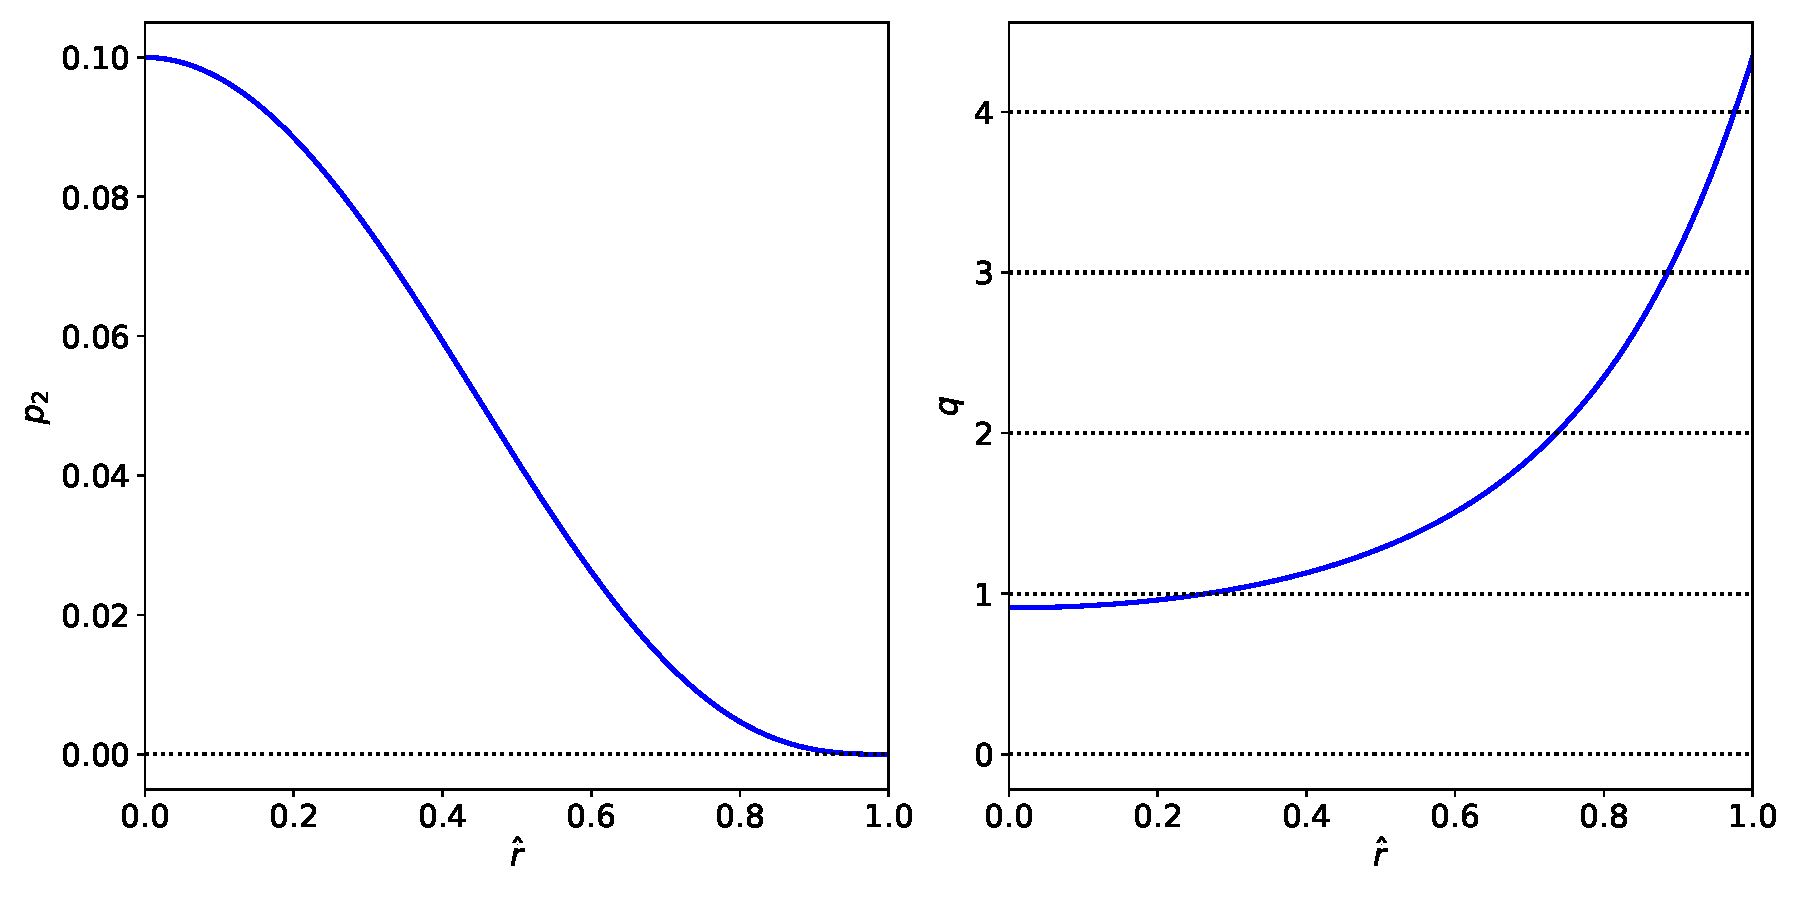
\includegraphics[width=0.9\textwidth]{Figure1.pdf}}
\caption{Normalized pressure and safety-factor profiles for the example tokamak equilibrium.}\label{f1}
\end{figure}

\begin{figure}
\centerline{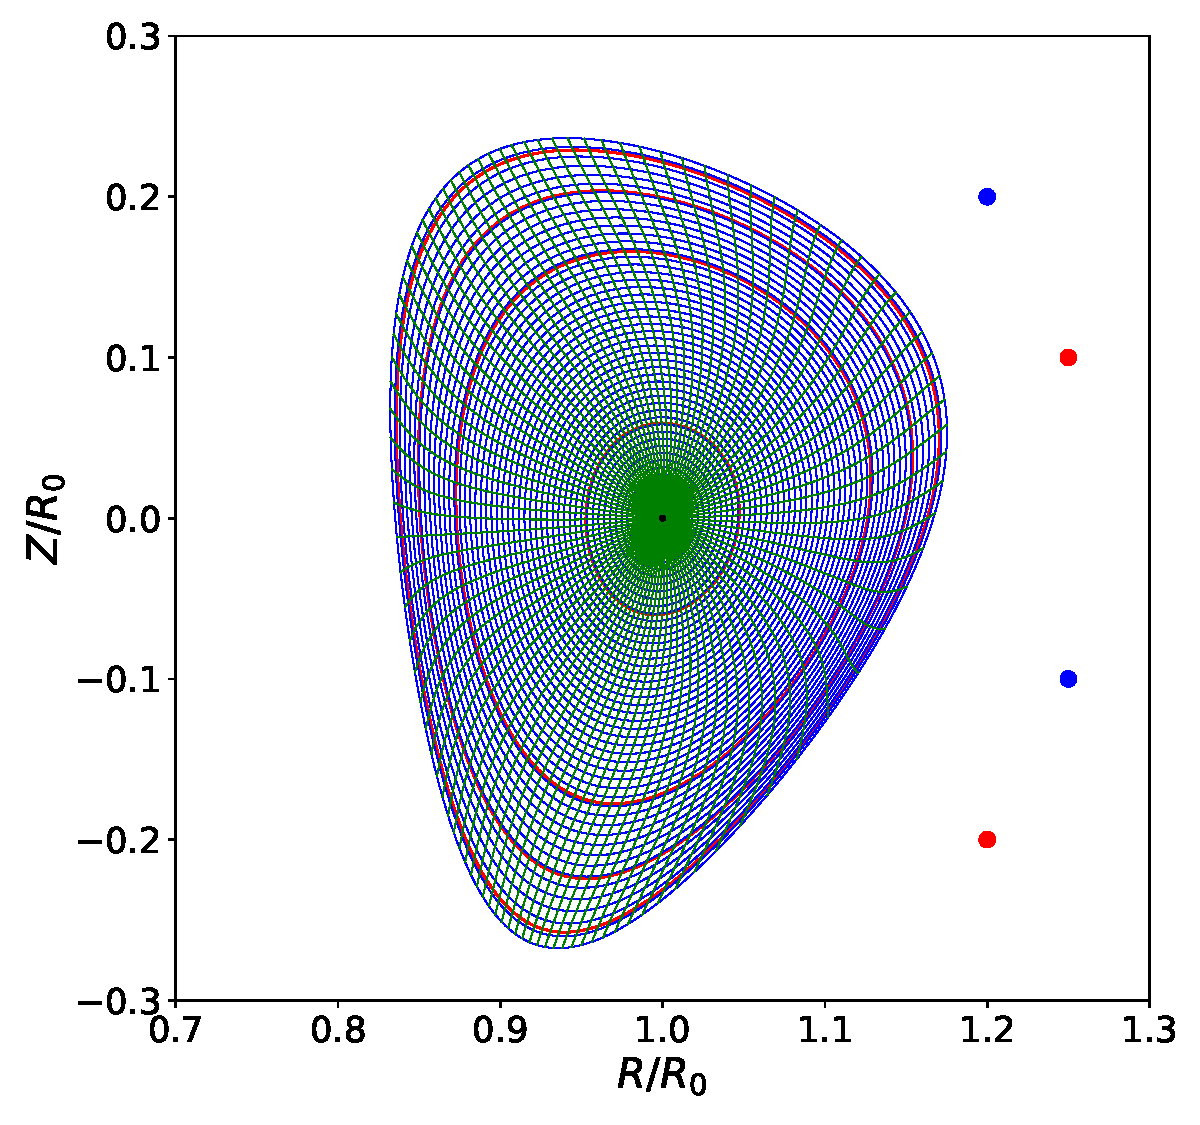
\includegraphics[width=0.8\textwidth]{Figure2.pdf}}
\caption{Flux-coordinate system calculated for the example tokamak equilibrium. Surfaces of constant $\hat{r}$ are shown as
blue curves, whereas surfaces of constant $\theta$ are shown as green curves. The red curves show the positions of the
four $n=1$ rational magnetic flux-surfaces in the plasma. The black dot shows the location of the magnetic axis. The
red and blue dots show the positions of the four toroidal strands that make up the RMP coil system. Blue indicates that the toroidal
current flowing in the strand is positive, whereas red indicates that it is negative. The magnitudes of the currents are equal.}\label{f2}
\end{figure}

\begin{figure}
\centerline{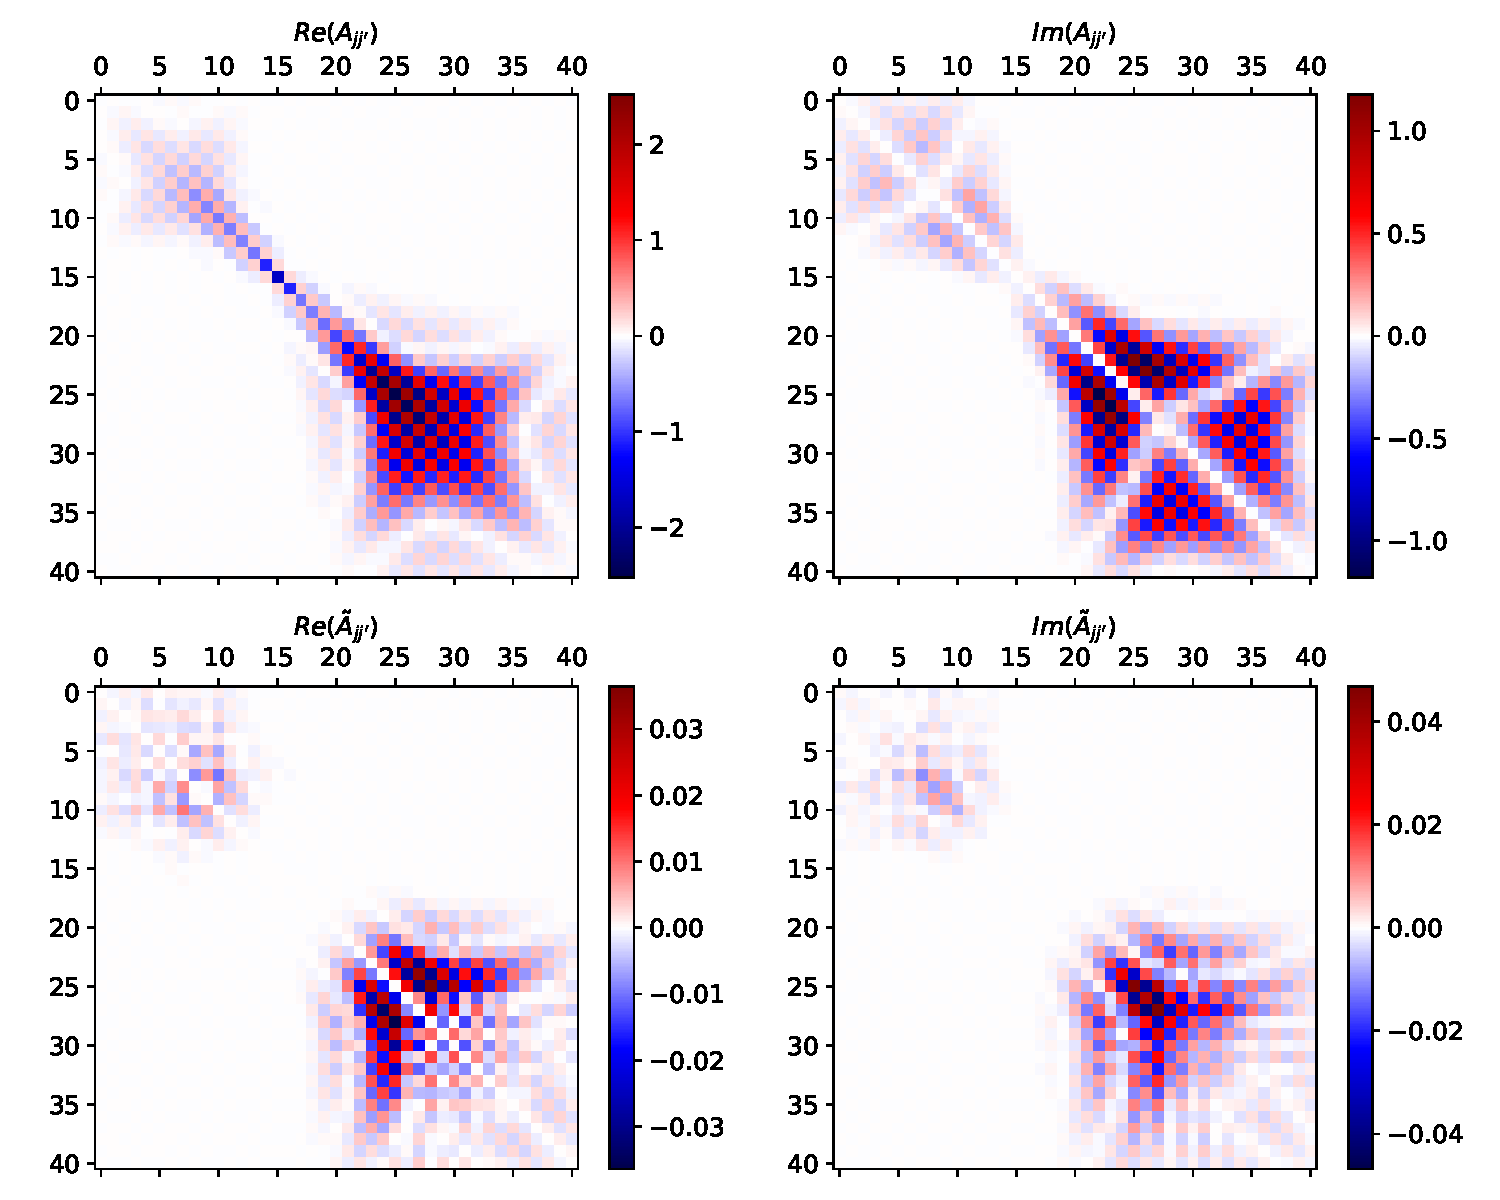
\includegraphics[width=\textwidth]{Figure3.pdf}}
\caption{Elements of the $n=1$ vacuum matrix $A_{jj'}$, as well as its anti-Hermitian component, $\tilde{A}_{jj''}$, calculated for the example
tokamak equilibrium specified in the previous two figures.}\label{f3}
\end{figure}

\begin{figure}
\centerline{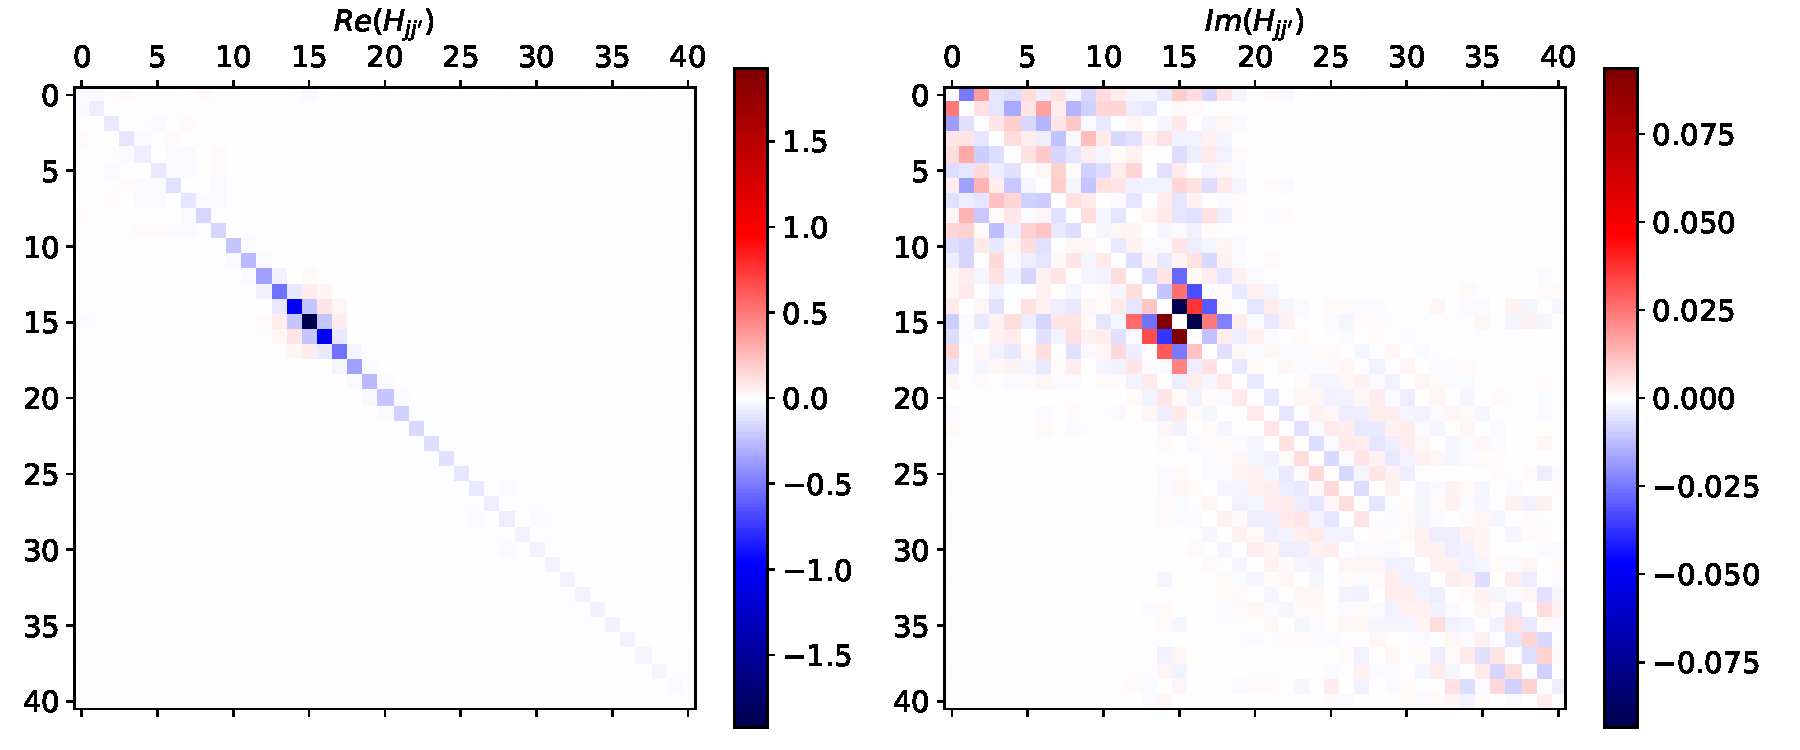
\includegraphics[width=\textwidth]{Figure4.pdf}}
\caption{Elements of the $n=1$ vacuum response  matrix, $H_{jj'}$, calculated for the example
tokamak equilibrium specified in Figs.~\ref{f1} and \ref{f2}.}\label{f4}
\end{figure}

\begin{figure}
\centerline{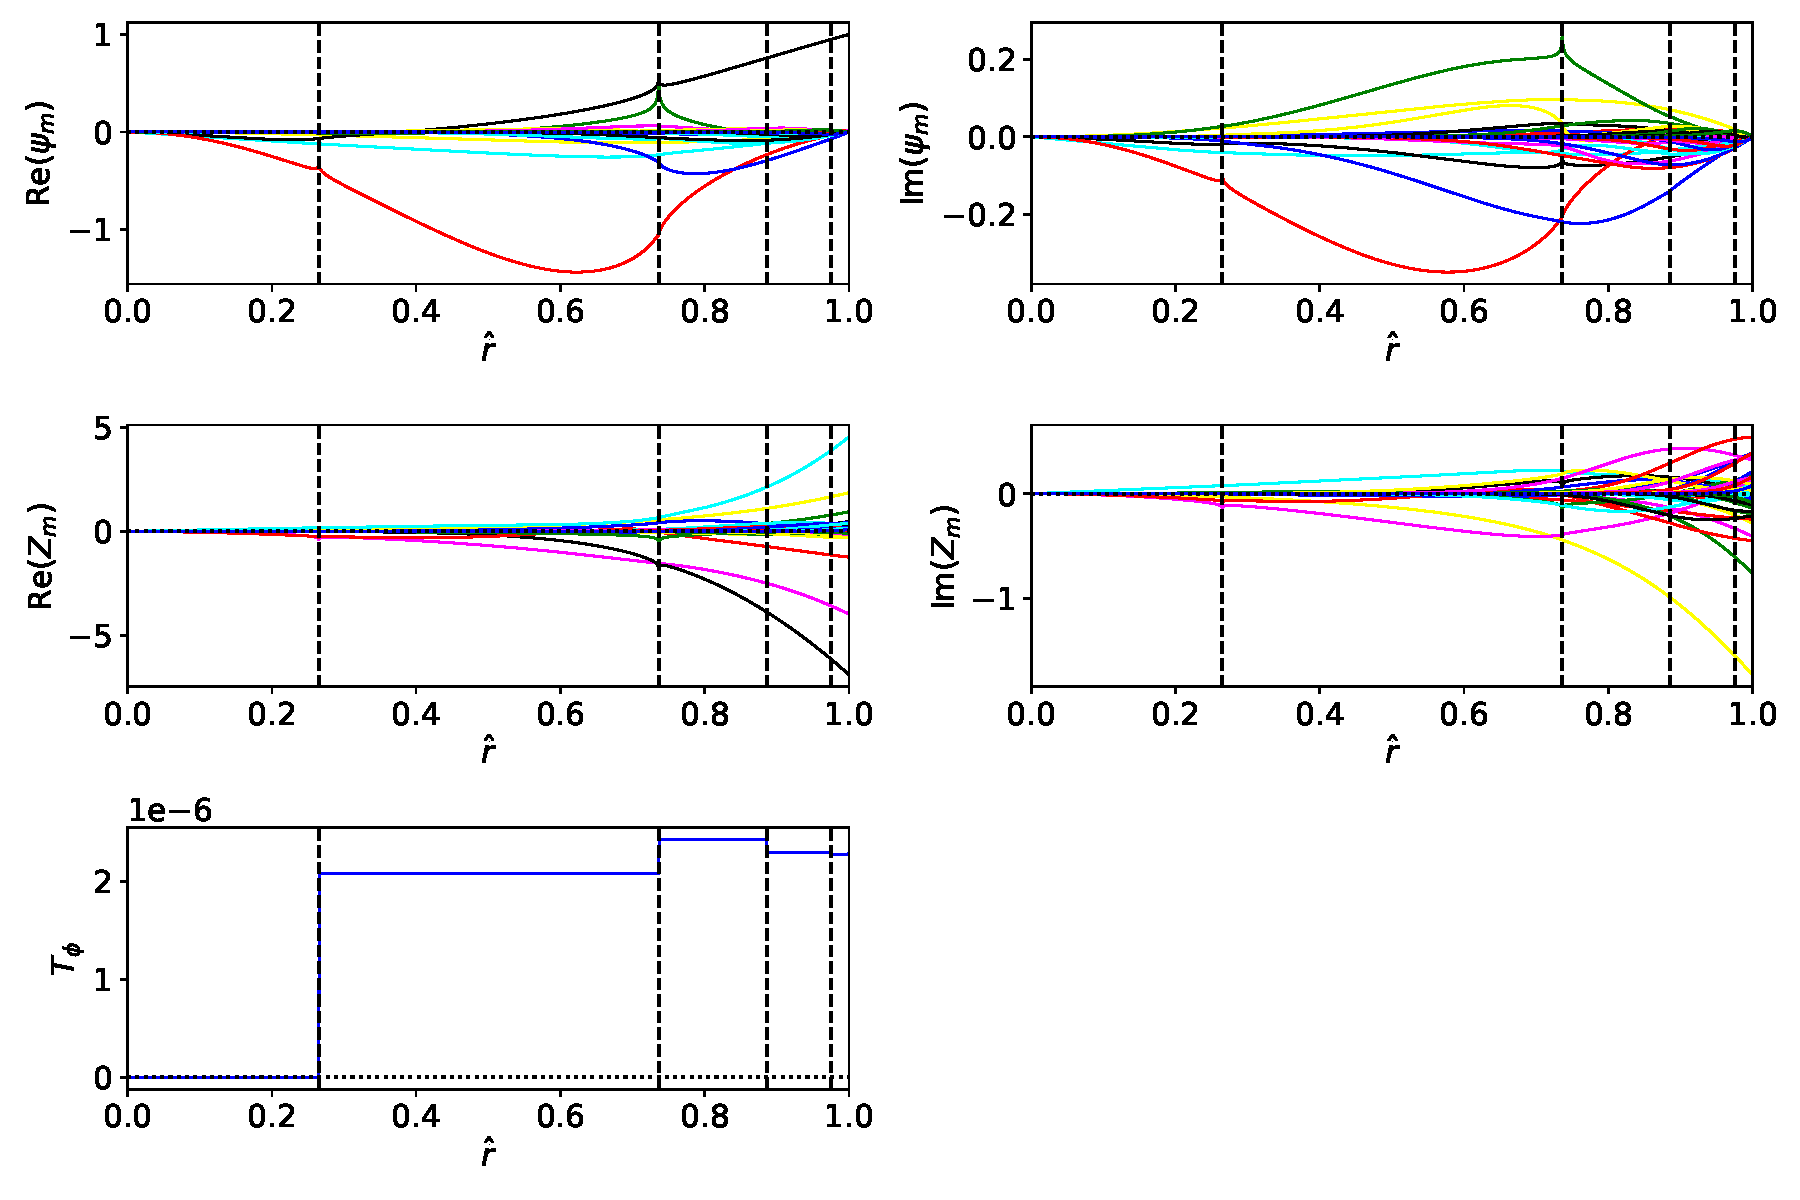
\includegraphics[width=\textwidth]{Figure5.pdf}}
\caption{Poloidal harmonics of a solution of the $n=1$ outer-region o.d.e.s, launched from the magnetic axis in such a manner that it is dominated by the $m=1$ harmonic close to the axis.
Black curves correspond to $m=1$, red to $m=0$ or $m=2$, green to $m=-1$ or $m=3$, blue to $m=-2$ or $m=4$, yellow to $m=-3$ or $m=5$,
cyan to $m=-4$ or $m=6$, magenta to $m=-5$ or $m=7$, black to $m=-6$ or $m=8$, et cetera. The vertical dashed lines show
the locations of the  $n=1$ rational surfaces. Here, $T_\phi(\hat{r})$ is the toroidal electromagnetic angular momentum 
flux associated with the solution.}\label{f5}
\end{figure}

\begin{figure}
\centerline{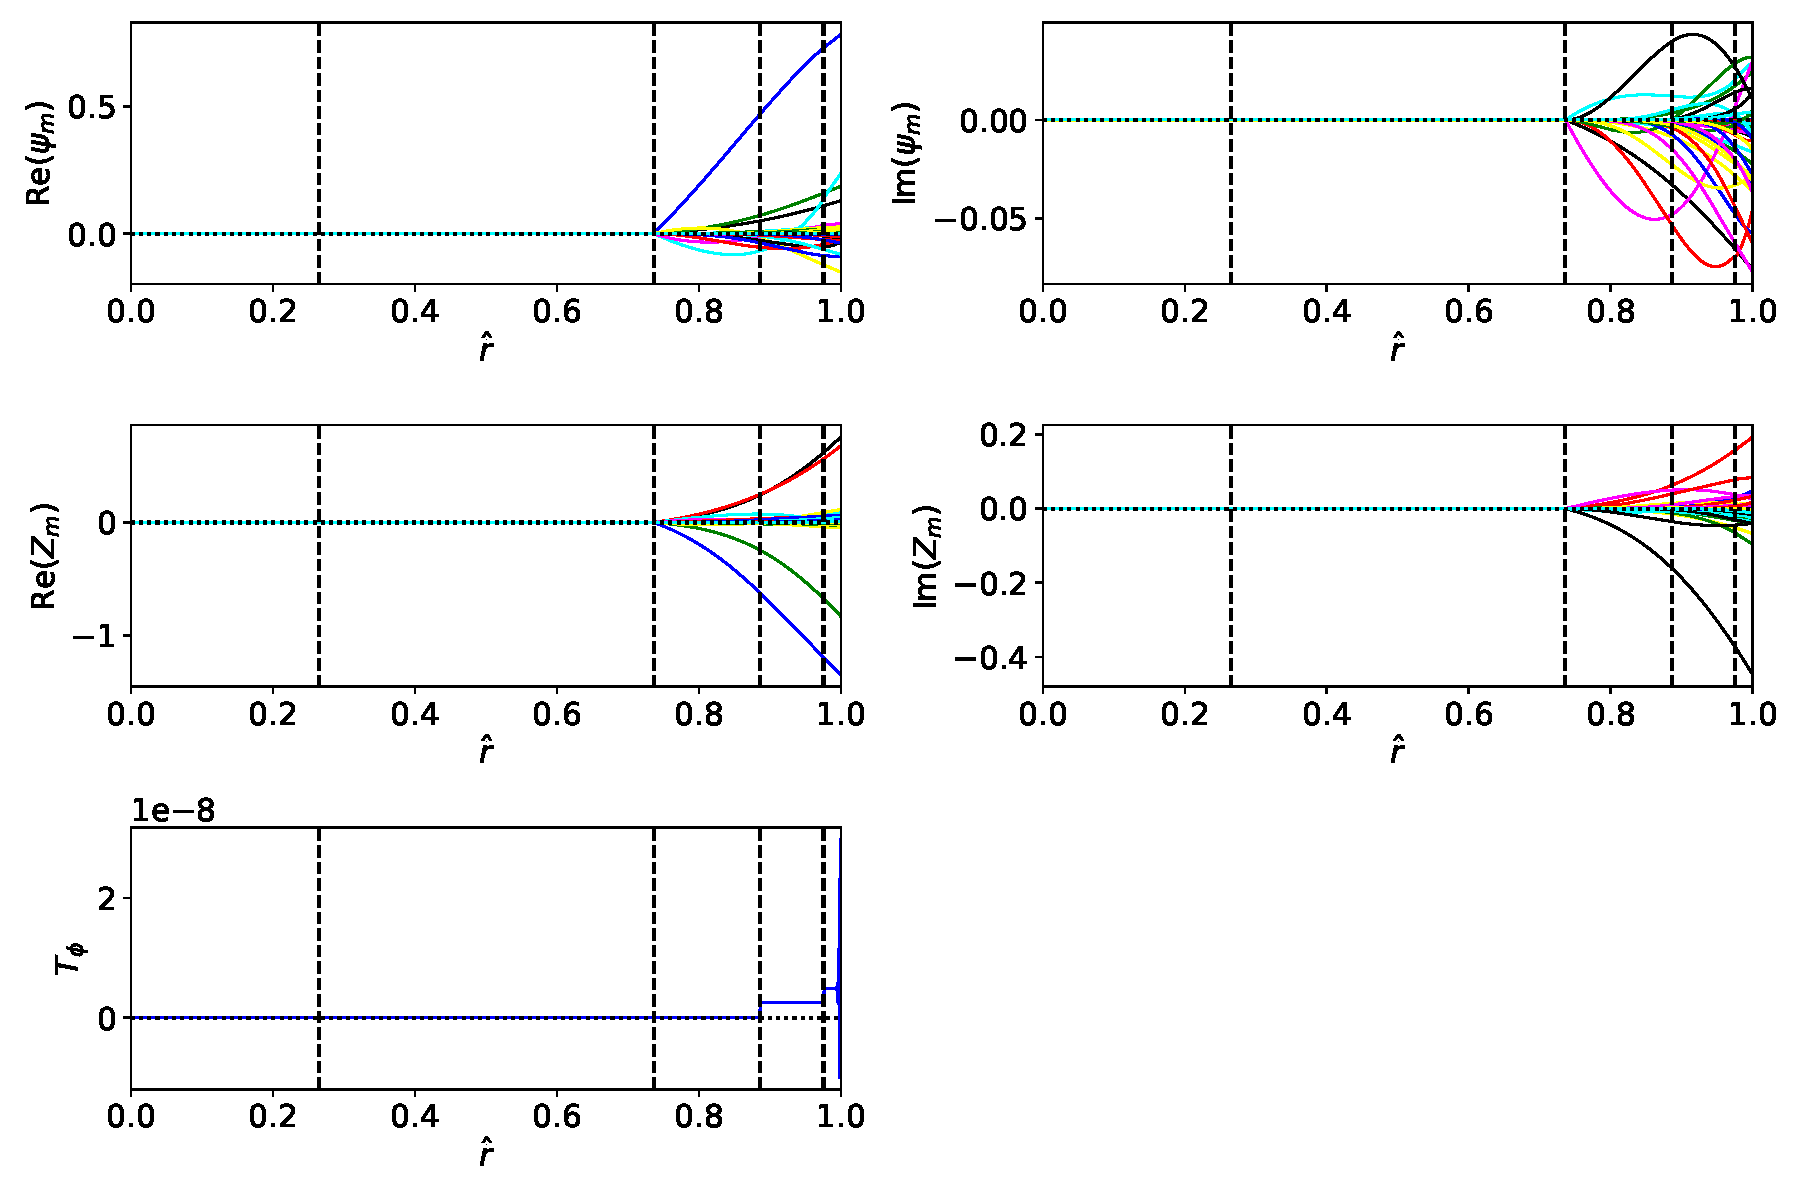
\includegraphics[width=\textwidth]{Figure6.pdf}}
\caption{Poloidal harmonics of a ``small'' solution of the $n=1$ outer-region o.d.e.s, launched from the $q=2$ surface.
Black curves correspond to $m=2$, red to $m=1$ or $m=3$, green to $m=0$ or $m=4$, blue to $m=-1$ or $m=5$, yellow to $m=-2$ or $m=6$,
cyan to $m=-3$ or $m=7$, magenta to $m=-4$ or $m=8$, black to $m=-5$ or $m=9$, et cetera. The vertical dashed lines show
the locations of the  $n=1$ rational surfaces. Here, $T_\phi(\hat{r})$ is the toroidal electromagnetic angular momentum 
flux associated with the solution.}\label{f6}
\end{figure}

\begin{figure}
\centerline{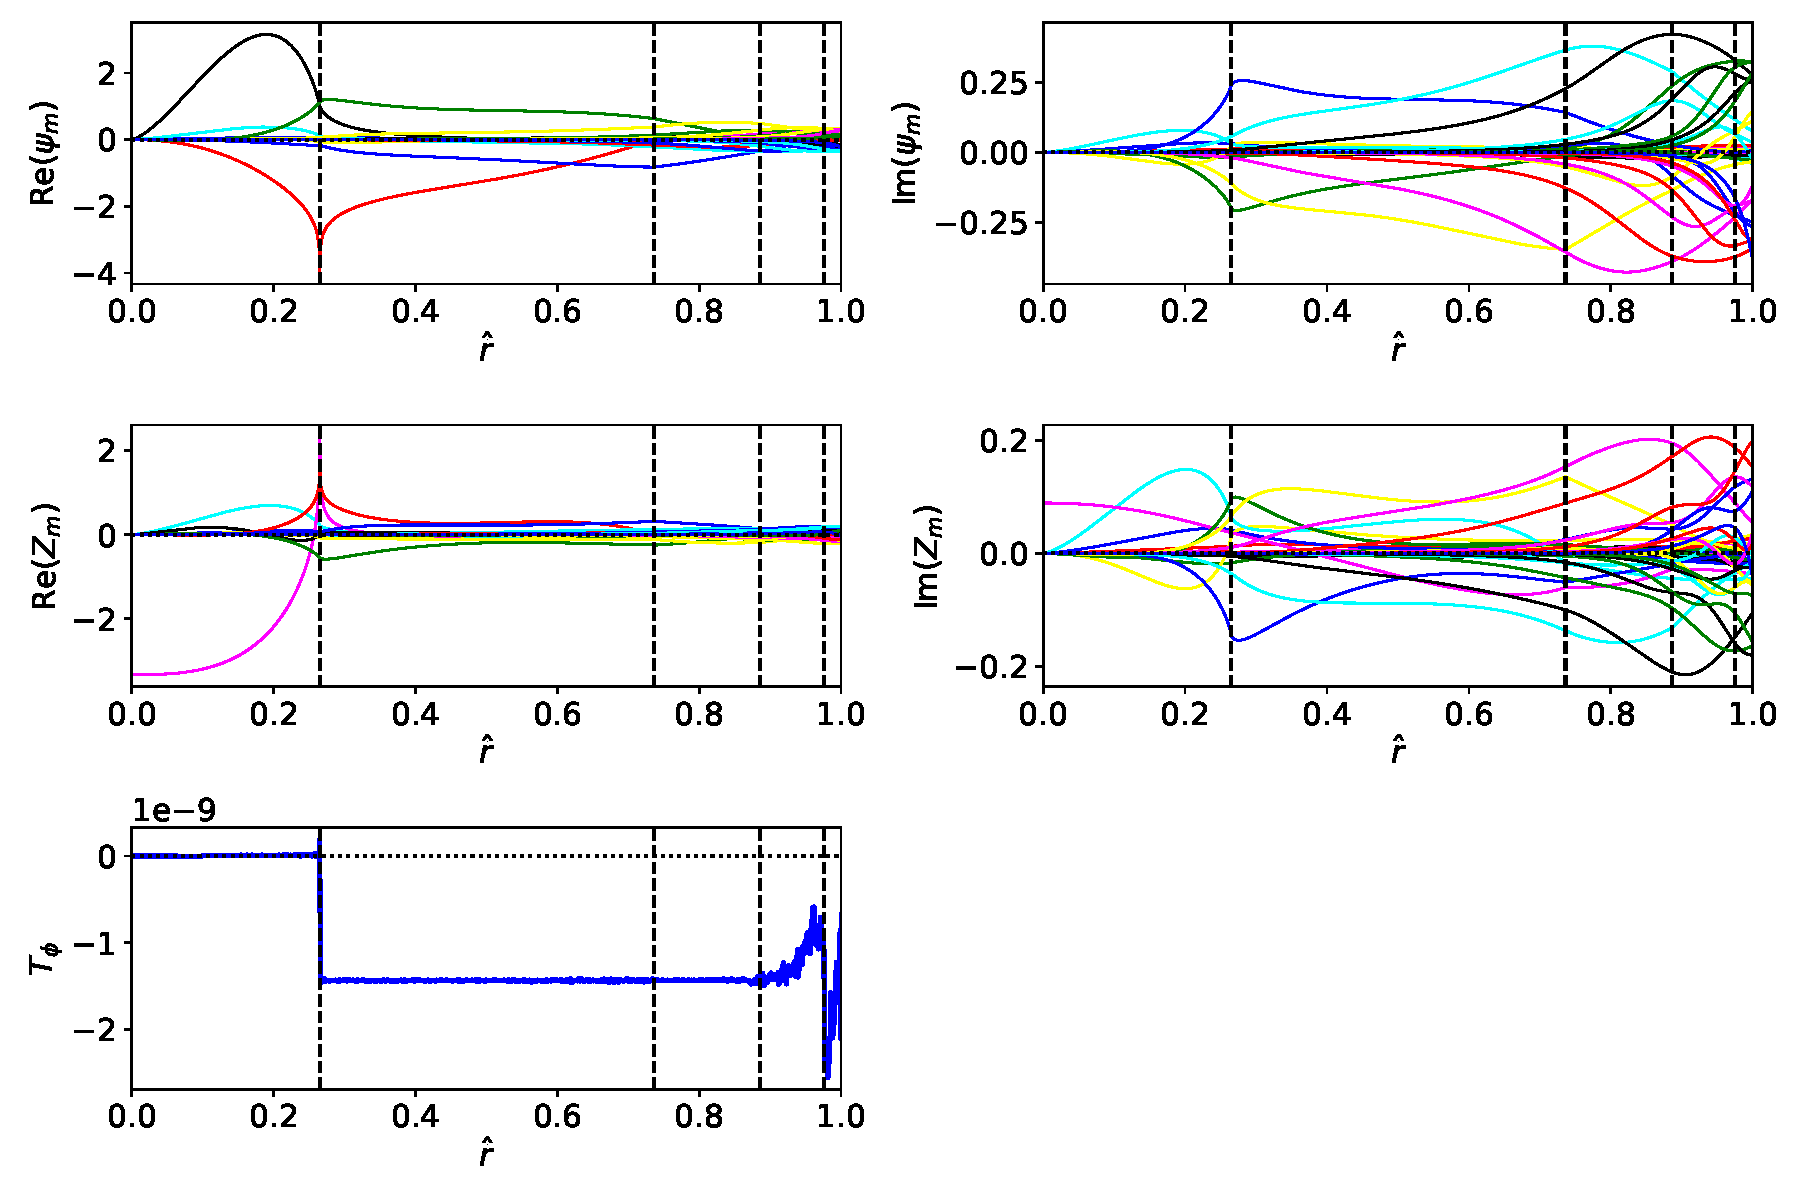
\includegraphics[width=\textwidth]{Figure7.pdf}}
\caption{Poloidal harmonics of the  ``unreconnected'' $n=1$ tearing eigenfunction associated with the $q=1$ surface. Black curves correspond to $m=1$, red to $m=0$ or $m=2$, green to $m=-1$ or $m=3$, blue to $m=-2$ or $m=4$, yellow to $m=-3$ or $m=5$,
cyan to $m=-4$ or $m=6$, magenta to $m=-5$ or $m=7$, black to $m=-6$ or $m=8$, et cetera. The vertical dashed lines show
the locations of the  $n=1$ rational surfaces.  Here, $T_\phi(\hat{r})$ is the toroidal electromagnetic angular momentum 
flux associated with the eigenfunction.}\label{f7}
\end{figure}

\begin{figure}
\centerline{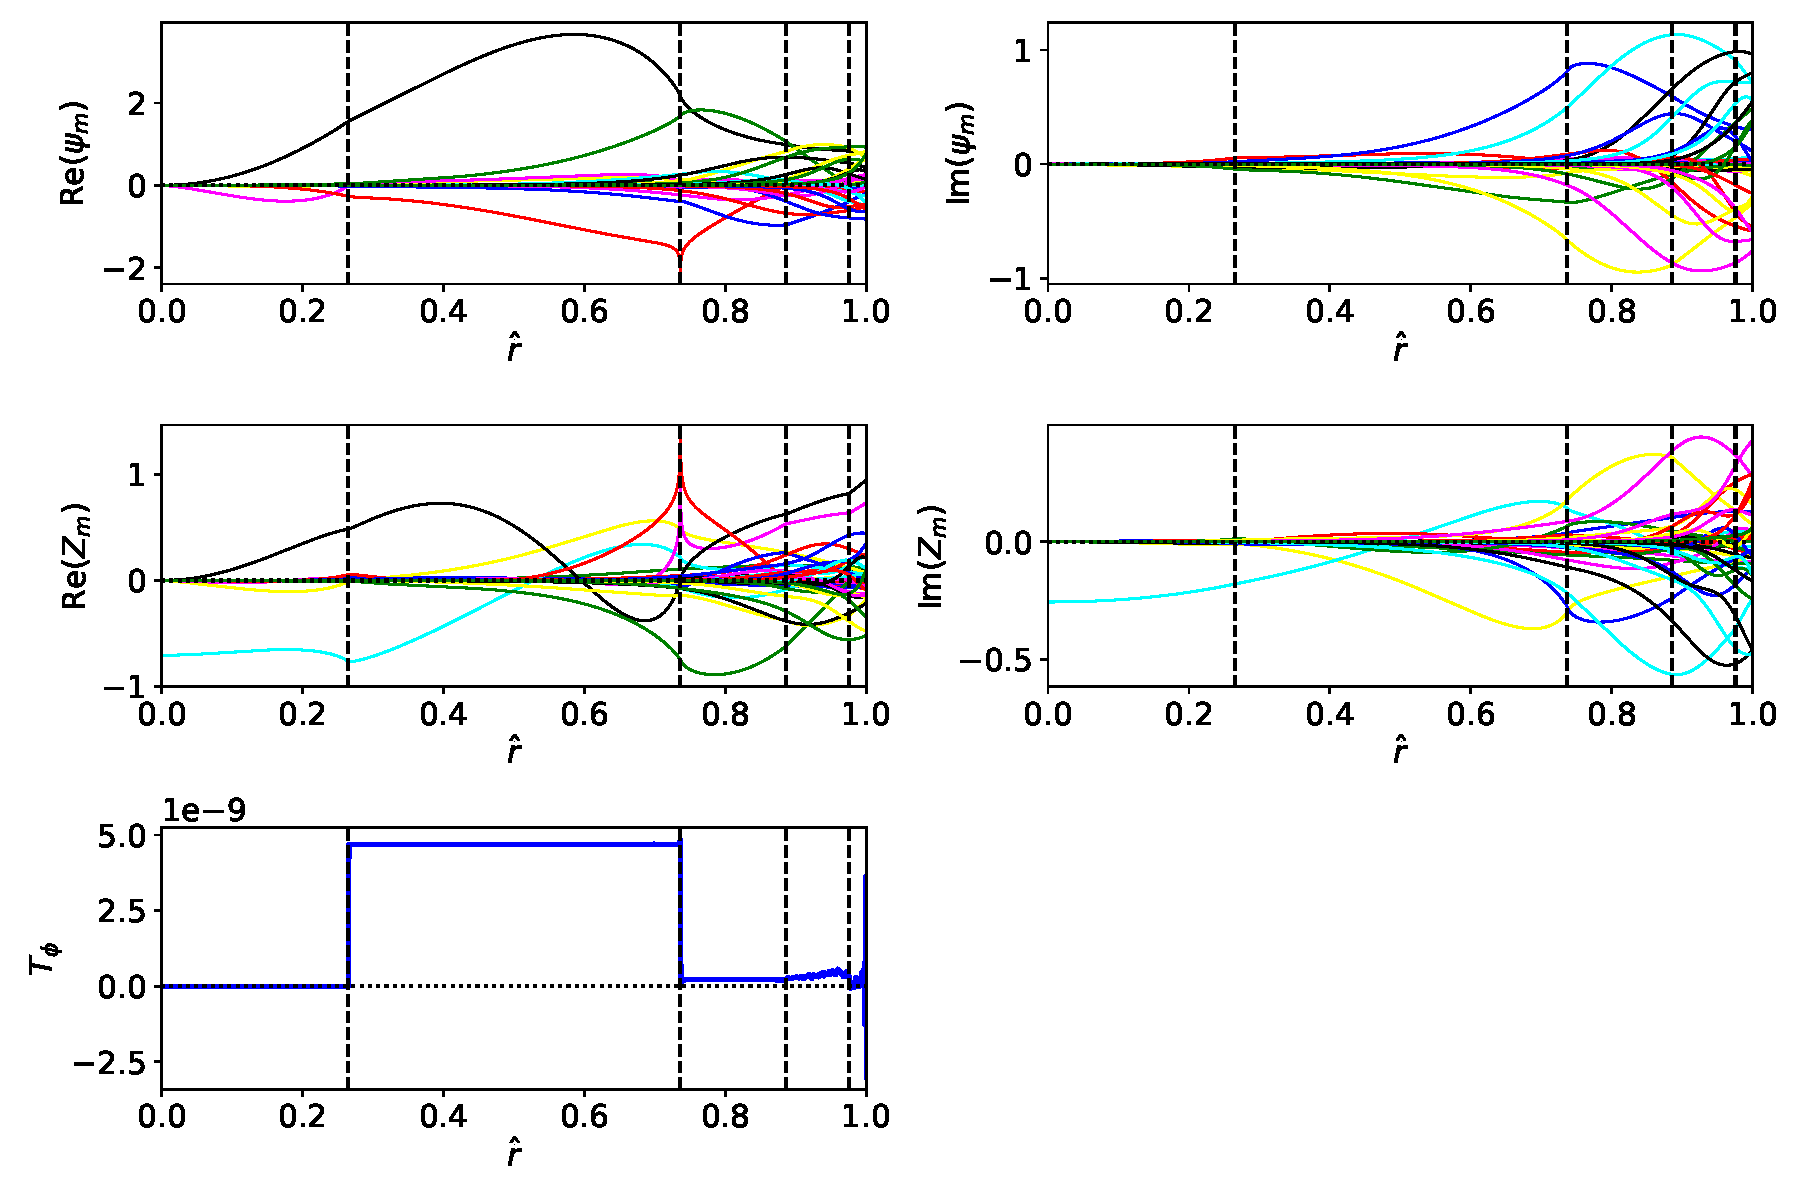
\includegraphics[width=\textwidth]{Figure8.pdf}}
\caption{Poloidal harmonics of the ``unreconnected'' $n=1$ tearing eigenfunction associated with the $q=2$ surface. Black curves correspond to $m=2$, red to $m=1$ or $m=3$, green to $m=0$ or $m=4$, blue to $m=-1$ or $m=5$, yellow to $m=-2$ or $m=6$,
cyan to $m=-3$ or $m=7$, magenta to $m=-4$ or $m=8$, black to $m=-5$ or $m=9$, et cetera.  The vertical dashed lines show
the locations of the  $n=1$ rational surfaces.  Here, $T_\phi(\hat{r})$ is the toroidal electromagnetic angular momentum 
flux associated with the eigenfunction.}\label{f8}
\end{figure}

\begin{figure}
\centerline{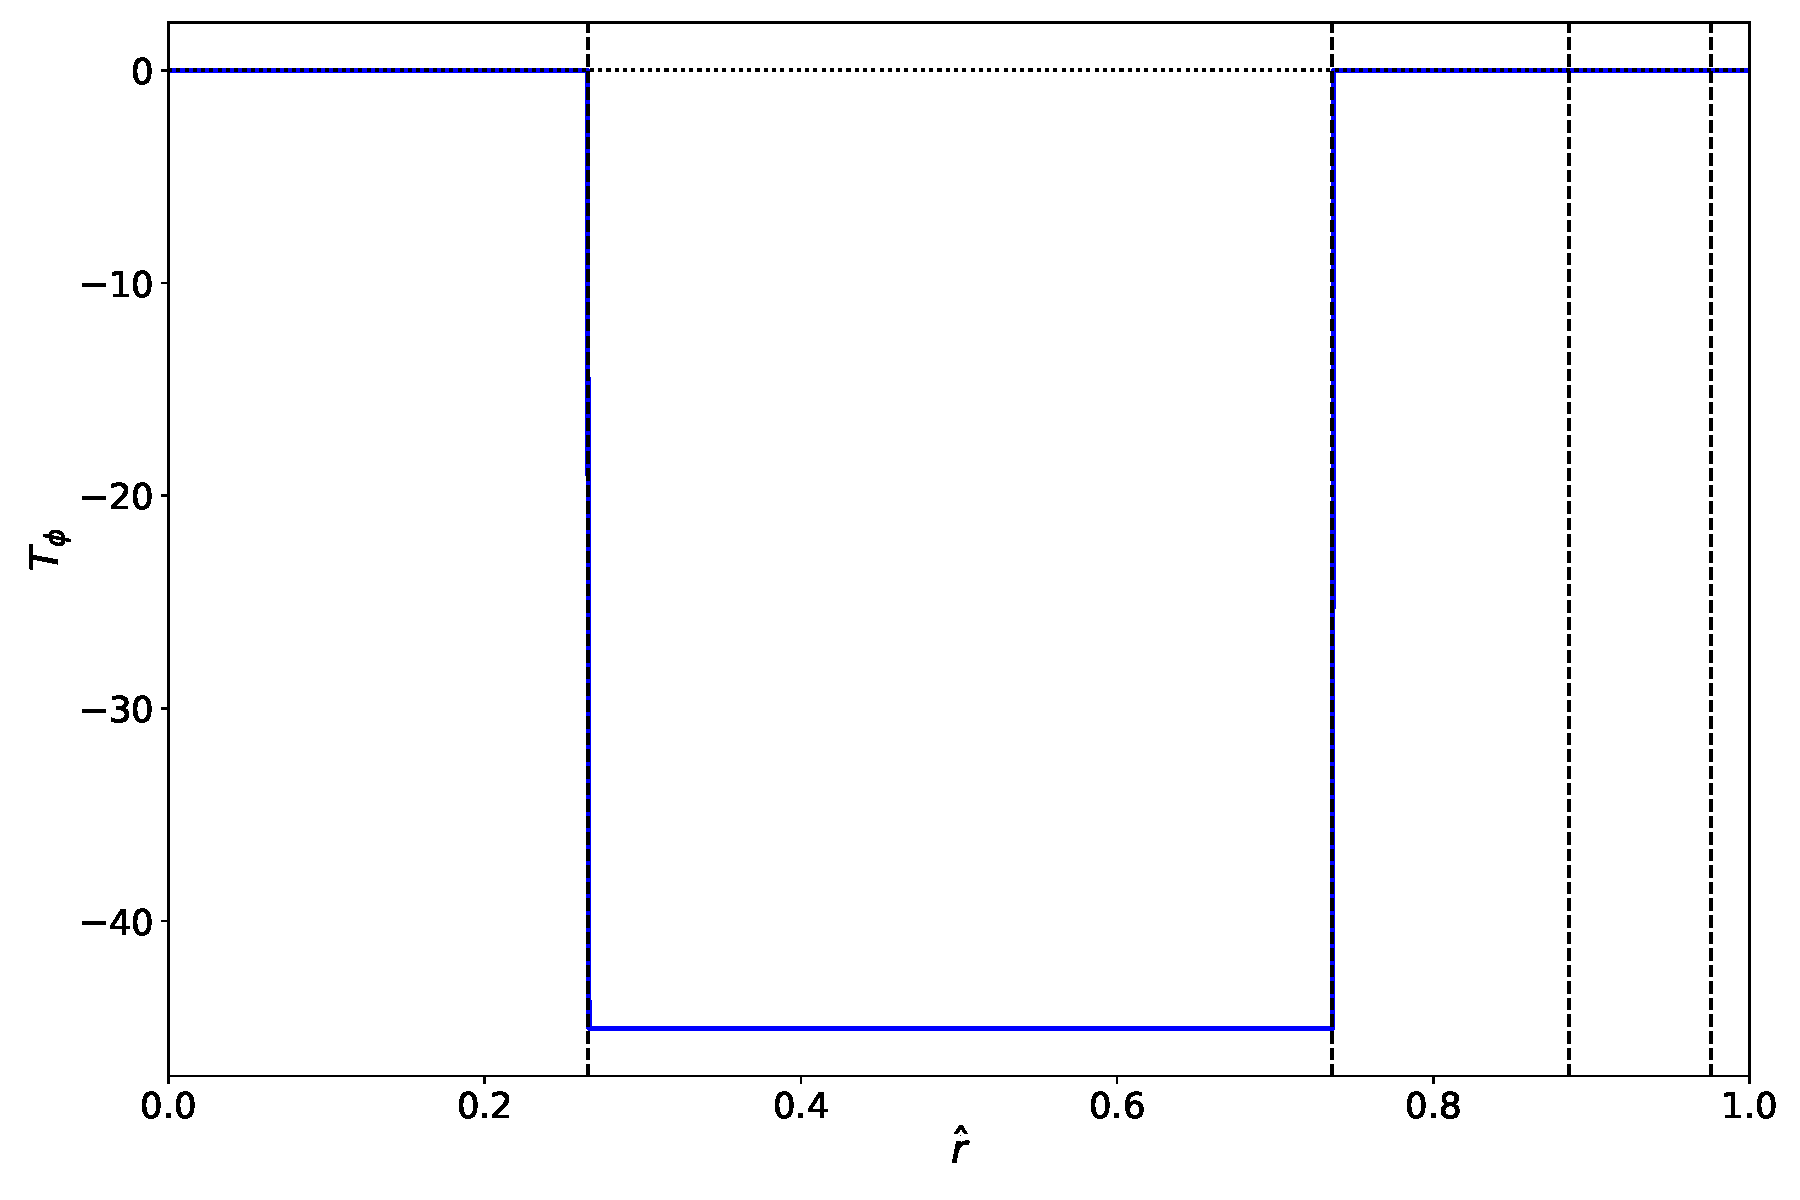
\includegraphics[width=0.9\textwidth]{Figure9.pdf}}
\caption{Toroidal electromagnetic  angular momentum flux associated with the tearing eigenfunction
pictured in Fig.~\ref{f7} added to ${\rm i}$ times the eigenfunction pictured in Fig.~\ref{f8}.  The vertical dashed lines show
the locations of the $n=1$ rational surfaces.  }\label{f9}
\end{figure}
\fi

\end{document}


